% ================================================================
% CHAPTERS 8--14: TRANSMISSION, FIXED POINTS, GEOMETRY, AND GAMES
% Expanded content for the IDT_Theory book (v2)
% ================================================================

% ================================================================
% CHAPTER 8: CHAINS OF TRANSMISSION
% ================================================================
\chapter{Chains of Transmission}
\label{ch:chains}

\epigraph{A word is dead when it is said, some say.  I say it just
begins to live that day.}{Emily Dickinson}

\section{From Dyads to Chains}

The preceding chapters studied the composition of \emph{two} ideas.  But ideas
in the real world rarely pass through only one intermediary.  A rumour travels
from mouth to mouth; a scientific result is cited, paraphrased, and summarised
across generations of papers; a joke is retold at party after party, acquiring
new inflections at each telling.  To model these phenomena we must study the
composition of \emph{chains}---sequences of ideas through which a signal is
transmitted.

Formally, composition is associative in the sense that the expression
$a \compose b_1 \compose b_2 \compose \cdots \compose b_n$ is well-defined by
iterated binary composition.  The question is: what happens to the weight,
resonance, and emergence as the chain grows?

\begin{definition}[Transmission Chain]
\label{def:chain}
Let $a \in \IS$ be a \textbf{source signal} and let
$\mathbf{b} = [b_1, b_2, \ldots, b_n]$ be a finite sequence of
\textbf{receivers} (or \textbf{contexts}).  The \textbf{transmission chain}
starting from $a$ through $\mathbf{b}$ is defined recursively:
\[
  \mathrm{chain}(a, [~]) := a,
  \qquad
  \mathrm{chain}(a, [b_1, \ldots, b_n])
    := \mathrm{chain}(a, [b_1, \ldots, b_{n-1}]) \compose b_n.
\]
We write $a^{\mathbf{b}} := \mathrm{chain}(a, \mathbf{b})$ for brevity, and
$|\mathbf{b}| := n$ for the \textbf{chain length}.
\end{definition}

\begin{remark}
The notation $a^{\mathbf{b}}$ should not be confused with iterated
self-composition $a^{\langle n \rangle}$; the superscript carries a bold-face
sequence, not a natural number.  When the chain is the constant sequence
$\mathbf{b} = [b, b, \ldots, b]$ of length $n$, we recover a special case of
iterated composition:
$a^{[b, \ldots, b]} = a \compose b^{\langle n \rangle}$ only when composition
is commutative, which it is not in general.
\end{remark}

\begin{interpretation}
\label{interp:ch8:bakhtin_chronotope}
The transmission chain formalises what Mikhail Bakhtin, in \emph{The Dialogic
Imagination} (1981), called the \textbf{chronotope}---the inseparability of
time and space in narrative.  For Bakhtin, every utterance carries the trace
of the spatial and temporal context in which it was produced; an idea cannot
be extracted from its chain of transmission any more than a word can be
extracted from its dialogic history.  Our formal chain
$\mathrm{chain}(a, [b_1, \ldots, b_n])$ makes this precise: the final idea
$a^{\mathbf{b}}$ is not merely $a$ ``plus'' its contexts, but the result of
\emph{sequential} composition in which order matters.  The chain is a
chronotope because each $b_i$ contributes not just content but a
\emph{position}---a moment in the sequence at which interpretation occurs.

The oral-formulaic theory of Milman Parry and Albert Lord provides a concrete
illustration.  In \emph{The Singer of Tales} (1960), Lord demonstrated that
Homeric epic was not memorised verbatim but \emph{recomposed in performance}
using formulaic phrases---``wine-dark sea,'' ``rosy-fingered dawn''---that
served as stable building blocks within a mutable compositional chain.  Each
performance by a \emph{guslar} (oral poet) constitutes a link $b_i$ in our
transmission chain.  The formulaic phrases are elements with high
self-resonance $w(b_i)$ that contribute predictable weight, while the
narrative structure undergoes creative mutation at each telling.  The Chain
Enrichment Theorem (Theorem~\ref{thm:chain-enrichment}) explains why these
epics grew in length and complexity across generations: each performance
added weight, even as fidelity to any ``original'' decreased.

G\'erard Genette's theory of narrative levels offers a third perspective.  In
\emph{Narrative Discourse} (1972), Genette distinguished between
\emph{diegesis} (the story world), \emph{metadiegesis} (a story within the
story), and \emph{extradiegesis} (the narrative act itself).  Each level
constitutes a retelling---a link in a transmission chain.  When Scheherazade
tells a story in which a character tells another story, we have a chain of
length~2; the inner story $a^{[b_1, b_2]}$ carries the weight of both
framing contexts.  Genette's insight that each narrative level transforms the
embedded narrative is precisely our observation that
$a^{[b_1, b_2]} \neq a^{[b_1]} \compose b_2'$ for $b_2' \neq b_2$: the
\emph{order} and \emph{identity} of the framing matters, not just the fact
of framing.
\end{interpretation}



\section{The Chain Enrichment Theorem}

The central result of this chapter asserts that transmission through a chain
can only \emph{increase} the weight of the transmitted idea.

\begin{theorem}[Chain Enrichment]
\label{thm:chain-enrichment}
For any source signal $a \in \IS$ and any chain
$\mathbf{b} = [b_1, \ldots, b_n]$,
\[
  w(a^{\mathbf{b}}) \geq w(a).
\]
That is, $\rs{a^{\mathbf{b}}}{a^{\mathbf{b}}} \geq \rs{a}{a}$.  The weight
is non-decreasing along the chain.
\end{theorem}

\begin{proof}
We proceed by induction on the chain length $n = |\mathbf{b}|$.

\textbf{Base case} ($n = 0$).  The chain is empty, so $a^{[~]} = a$ and
$w(a^{[~]}) = w(a)$.  The inequality holds with equality.

\textbf{Inductive step.}  Assume the result holds for all chains of length
$n - 1$.  Write
$\mathbf{b}' = [b_1, \ldots, b_{n-1}]$, so that
$a^{\mathbf{b}} = a^{\mathbf{b}'} \compose b_n$.
By the inductive hypothesis,
\[
  w(a^{\mathbf{b}'}) \geq w(a).
\]
Now apply axiom \textbf{E4} (Composition Enriches) to the pair
$(a^{\mathbf{b}'}, b_n)$:
\[
  w(a^{\mathbf{b}'} \compose b_n)
  = w(a^{\mathbf{b}})
  \geq w(a^{\mathbf{b}'})
  \geq w(a).
\]
This completes the induction.
\end{proof}

In Lean~4, the proof follows the same inductive structure:

\begin{lstlisting}
theorem chain_enrichment (a : Idea) (bs : List Idea) :
    w (chain a bs) >= w a := by
  induction bs with
  | nil => simp [chain, w]
  | cons b bs' ih =>
    simp [chain]
    calc w (chain a bs' |> (. @\compose@ b))
        >= w (chain a bs') := composition_enriches _ _
      _ >= w a := ih
\end{lstlisting}

\begin{interpretation}
\label{int:chain-enrichment}
The Chain Enrichment Theorem is the mathematical expression of a surprising
anthropological observation: \emph{ideas grow heavier through transmission,
never lighter.}  In the classic ``telephone game,'' a message is whispered
from person to person around a circle, and the final message is typically
very different from the original.  The na\"{i}ve expectation is that the message
\emph{degrades}---that information is lost at each step.

But ``degradation'' is not the same as ``weight loss.''  The weight
$w(a) = \rs{a}{a}$ measures the self-resonance of an idea, its internal
richness and complexity.  Each retelling adds the receiver's context, and
axiom E4 guarantees that this addition can only increase total weight.
The \emph{content} may change---the original message may be unrecognisable---but
the \emph{weight} of the cultural artefact only grows.

This theorem explains why rumours grow more elaborate, why myths accumulate
detail over centuries, and why urban legends become more vivid with each
retelling.  The message mutates, but the mutation always adds weight.  It is
as if each retelling deposits a sedimentary layer: the original may be
buried, but the total mass only increases.
\end{interpretation}

\begin{interpretation}
\label{interp:ch8:derrida_iterability}
The Chain Enrichment Theorem bears a deep connection to Jacques Derrida's
concept of \textbf{iterability}, developed in ``Signature Event Context''
(1972) and \emph{Limited Inc} (1988).  Derrida argued that every sign, by
its very nature, must be \emph{repeatable}---iterable---in new contexts, and
that this repetition necessarily introduces \emph{diff\'erance}: a
simultaneous differing and deferring of meaning.  ``A written sign carries
with it a force that breaks with its context,'' Derrida wrote, ``that is,
with the collectivity of presences organising the moment of its inscription.''

Our theorem gives this claim a precise mathematical form.  When an idea $a$
is transmitted through a chain $[b_1, \ldots, b_n]$, each composition
$a^{[b_1,\ldots,b_k]} \compose b_{k+1}$ is an act of iteration: the idea is
repeated in a new context $b_{k+1}$.  The theorem guarantees that this
iteration always \emph{enriches}---weight increases---but the enrichment is
precisely the ``force that breaks with context'' that Derrida identified.
The original idea $a$ is \emph{deferred} (its direct contribution is
progressively buried under accumulated emergence) and \emph{differed from}
(the final idea $a^{\mathbf{b}}$ may bear no resemblance to $a$).  Yet the
weight---the total self-resonance---only grows.

Ludwig Wittgenstein's \textbf{rule-following paradox} (\emph{Philosophical
Investigations}, \S\S185--202) illuminates a different aspect.
Wittgenstein asked: what determines that a rule has been followed correctly?
Each step in following a rule requires an act of interpretation, and no finite
set of examples can determine the rule uniquely.  In our framework, each link
$b_i$ in the chain is an interpretive act---an application of the ``rule'' of
the original idea $a$.  The Chain Enrichment Theorem shows that each such
application adds weight, but the paradox remains: there is no formal
guarantee that the ``rule'' followed at step $i$ is the ``same'' rule
intended at step $1$.  The chain enriches, but it does not conserve direction.

Hans-Georg Gadamer's \textbf{effective-historical consciousness}
(\emph{wirkungsgeschichtliches Bewu\ss{}tsein}), developed in \emph{Truth
and Method} (1960), provides the hermeneutic perspective.  Gadamer argued
that we never encounter a text or idea in isolation; we always encounter it
through the chain of its effects---its \emph{Wirkungsgeschichte}.  To
understand Homer is to understand Homer \emph{as received through} two
millennia of commentary, translation, and pedagogical transmission.  The
chain $a^{[b_1,\ldots,b_n]}$ \emph{is} the effective-historical reality of
the idea $a$: we cannot strip away the chain to recover the ``original''
because the chain \emph{is} how the idea exists for us.  The enrichment
theorem confirms Gadamer's fundamental insight: tradition does not degrade
meaning; it enriches it.
\end{interpretation}



\section{Cumulative Emergence Along Chains}

The Chain Enrichment Theorem tells us about weight; we now ask about the
\emph{structure} of the enrichment.  How does emergence accumulate?

\begin{definition}[Cumulative Emergence]
\label{def:cumulative-emergence}
The \textbf{cumulative emergence} of a chain $(a, \mathbf{b})$ with respect
to observer $c$ is:
\[
  E_{\mathrm{cum}}(a, \mathbf{b}, c)
  := \rs{a^{\mathbf{b}}}{c} - \rs{a}{c}
     - \sum_{i=1}^{n} \rs{b_i}{c}.
\]
\end{definition}

\begin{remark}
\label{rem:ch8:cumulative_emergence_herder}
The concept of cumulative emergence recalls Johann Gottfried Herder's
philosophy of cultural history (\emph{Ideas on the Philosophy of the
History of Mankind}, 1784--91).  Herder argued that each nation and epoch
contributes something unique to the collective treasury of humanity, and
that this collective treasury is \emph{more} than the sum of its parts.
The cumulative emergence $E_{\mathrm{cum}}(a, \mathbf{b}, c)$ is the
mathematical formalisation of Herder's ``surplus''---the meaning that the
chain of cultural transmission produces beyond what any individual link
could contribute alone.  Herder's insight that ``each nation bears in itself
the standard of its perfection, totally independent of all comparison with
that of others'' is the observation that cumulative emergence depends on
the observer $c$: different observers see different surpluses in the same
chain of transmission.
\end{remark}



\begin{theorem}[Emergence Decomposition for Chains]
\label{thm:emergence-decomposition}
The cumulative emergence decomposes as a sum of local emergences:
\[
  E_{\mathrm{cum}}(a, \mathbf{b}, c)
  = \sum_{i=1}^{n}
    \emerge\!\left(
      a^{[b_1, \ldots, b_{i-1}]},\, b_i,\, c
    \right),
\]
where $\emerge(x, y, c) := \rs{x \compose y}{c} - \rs{x}{c} - \rs{y}{c}$ is
the emergence at a single composition step, with the ``current accumulated
idea'' $a^{[b_1, \ldots, b_{i-1}]}$ as the left operand.
\end{theorem}

\begin{proof}
We proceed by induction on $n$.

\textbf{Base case} ($n = 1$).
$E_{\mathrm{cum}}(a, [b_1], c) = \rs{a \compose b_1}{c} - \rs{a}{c} - \rs{b_1}{c}
= \emerge(a, b_1, c)$.

\textbf{Inductive step.}
Write $\mathbf{b}' = [b_1, \ldots, b_{n-1}]$ and $p = a^{\mathbf{b}'}$.
Then $a^{\mathbf{b}} = p \compose b_n$, and
\begin{align*}
  E_{\mathrm{cum}}(a, \mathbf{b}, c)
  &= \rs{p \compose b_n}{c} - \rs{a}{c}
     - \sum_{i=1}^{n} \rs{b_i}{c} \\
  &= \bigl[\rs{p \compose b_n}{c} - \rs{p}{c} - \rs{b_n}{c}\bigr]
     + \rs{p}{c} - \rs{a}{c}
     - \sum_{i=1}^{n-1} \rs{b_i}{c} \\
  &= \emerge(p, b_n, c) + E_{\mathrm{cum}}(a, \mathbf{b}', c) \\
  &= \emerge(p, b_n, c)
     + \sum_{i=1}^{n-1} \emerge\!\left(
         a^{[b_1, \ldots, b_{i-1}]}, b_i, c
       \right) \quad\text{(by induction)}\\
  &= \sum_{i=1}^{n} \emerge\!\left(
       a^{[b_1, \ldots, b_{i-1}]}, b_i, c
     \right). \qedhere
\end{align*}
\end{proof}

\begin{interpretation}
The cumulative emergence is the \emph{total surplus of meaning} that the chain
has produced beyond the mere sum of its parts.  Each link in the chain
contributes a local emergence $\emerge(p_i, b_{i+1}, c)$, which depends on the
\emph{entire accumulated idea} at that point, not just the original signal.
This is the formal content of the observation that ``context matters'': the
emergence at step~$i$ depends on everything that came before.

When cumulative emergence is large and positive, the chain has been
\emph{synergistic}---the ideas have reinforced each other in ways that
transcend their individual contributions.  When it is negative, the chain
has been \emph{destructive}---meaning has been lost to interference.  The
Chain Enrichment Theorem tells us that total weight still increases, but
the resonance with any particular observer $c$ may decrease: the idea may
grow heavier while becoming less relevant to any given perspective.
\end{interpretation}

\begin{interpretation}
\label{interp:ch8:peirce_interpretants}
The Emergence Decomposition Theorem provides the mathematical infrastructure
for Charles Sanders Peirce's theory of the \textbf{chain of interpretants}.
In Peirce's semiotics, every sign produces an \emph{interpretant}---another
sign that interprets the first---and this interpretant in turn produces its
own interpretant, creating an infinite chain of semiosis.  ``The meaning of a
representation can be nothing but a representation,'' Peirce wrote in the
\emph{Collected Papers} (5.252).

Our decomposition shows that the cumulative emergence along the chain
$E_{\mathrm{cum}}(a, \mathbf{b}, c) = \sum_i \emerge(a^{[b_1,\ldots,b_{i-1}]}, b_i, c)$
is the total \emph{surplus of meaning} produced by the chain of
interpretants.  Each local emergence $\emerge(p_i, b_{i+1}, c)$ is the
contribution of the $i$-th interpretant: the new meaning that arises from
interpreting the accumulated sign $p_i$ in the context $b_{i+1}$.  Peirce's
insight that each interpretant depends on the \emph{entire previous chain}
(not just the original sign) is captured by the fact that $p_i = a^{[b_1,\ldots,b_i]}$
is the full accumulated idea, not merely $a$.

Yuri Lotman's concept of the \textbf{semiosphere}---the totality of semiotic
acts in a culture, developed in \emph{Universe of the Mind} (1990)---adds
a diachronic dimension.  Lotman argued that the semiosphere has a temporal
axis along which signs are transmitted and transformed.  The chain
$(a, \mathbf{b})$ models a trajectory through Lotman's semiosphere: the idea
$a$ enters the semiotic space and is progressively transformed by the
cultural contexts $b_1, b_2, \ldots$ it encounters.  The cumulative emergence
$E_{\mathrm{cum}}$ measures the total semiotic work performed along this
trajectory---the total meaning generated by the semiosphere's processing of
the idea.

It is instructive to compare our framework with Claude Shannon's
\emph{mathematical theory of communication} (1948).  In Shannon's theory,
a channel is characterised by a transition probability $p(y|x)$, and the
goal is to transmit information with minimal error.  Emergence is identically
zero in Shannon's framework ($\kappa = 0$ in our notation): the channel adds
noise but no \emph{meaning}.  The transmission chain in Shannon's theory is
a Markov chain, where each step depends only on the current state.  Our
framework generalises Shannon's by allowing each transmission step to produce
\emph{genuine emergence}---meaning that was not present in either the signal
or the channel.  Shannon's theory is the degenerate case where cultural
transmission reduces to signal processing; IDT captures the full richness of
meaning-making that information theory deliberately abstracts away.
\end{interpretation}



\section{The Ratchet Effect}

\begin{definition}[Weight Sequence]
\label{def:weight-sequence}
The \textbf{weight sequence} of a chain $(a, \mathbf{b})$ is the sequence
\[
  W_0 := w(a), \quad
  W_k := w(a^{[b_1, \ldots, b_k]}) \quad (k = 1, \ldots, n).
\]
\end{definition}

\begin{corollary}[The Ratchet Effect]
\label{cor:ratchet}
The weight sequence is non-decreasing:
$W_0 \leq W_1 \leq W_2 \leq \cdots \leq W_n$.
Moreover, $W_k = W_{k-1}$ if and only if
$\emerge(a^{[b_1, \ldots, b_{k-1}]}, b_k, a^{[b_1, \ldots, b_k]}) = -\rs{b_k}{a^{[b_1,\ldots,b_k]}}$.
\end{corollary}

\begin{remark}
\label{rem:ch8:ratchet_entropy}
The Ratchet Effect stands in instructive contrast to the second law of
thermodynamics, which states that entropy (disorder) can only increase in
a closed system.  The cultural ratchet says that \emph{weight} (a measure
of complexity or richness) can only increase along a transmission chain.
Both are irreversibility results, but they point in opposite directions:
thermodynamic entropy measures \emph{disorder}, while ideatic weight measures
\emph{complexity}.  The apparent paradox---that both disorder and complexity
increase monotonically---is resolved by noting that the ideatic space is
not a closed thermodynamic system.  Each receiver $b_i$ is a source of
negentropy (structured information) that is injected into the chain,
driving weight upward even as the physical substrate may be degrading.
This is precisely Erwin Schr\"odinger's insight in \emph{What is Life?}
(1944): living systems maintain and increase their complexity by importing
negentropy from their environment.
\end{remark}



\begin{proof}
Monotonicity follows from E4 applied at each step.  For the equality
condition, $W_k = W_{k-1}$ means
$w(p \compose b_k) = w(p)$ where $p = a^{[b_1,\ldots,b_{k-1}]}$.
Since $w(p \compose b_k) = \rs{p \compose b_k}{p \compose b_k}
= \rs{p}{p \compose b_k} + \rs{b_k}{p \compose b_k}
  + \emerge(p, b_k, p \compose b_k)$,
the condition $w(p \compose b_k) = w(p)$ gives
$\rs{b_k}{p \compose b_k} + \emerge(p, b_k, p \compose b_k)
= w(p) - \rs{p}{p \compose b_k}$,
from which the stated condition follows after rearrangement.
\end{proof}

\begin{remark}
The name ``ratchet'' comes from the mechanical device that permits motion in
only one direction.  Cultural weight, like a ratchet, clicks forward but
never backward.  This is the formal analogue of the ``cultural ratchet
effect'' discussed by Tomasello (1999) in the context of cumulative culture.
\end{remark}

\begin{interpretation}
\label{interp:ch8:tomasello_ratchet}
The Ratchet Effect (Corollary~\ref{cor:ratchet}) formalises what Michael
Tomasello, in \emph{The Cultural Origins of Human Cognition} (1999), called
the \textbf{cultural ratchet}: the mechanism by which human cultures
accumulate complexity over generations in a way that no other species matches.
Tomasello observed that chimpanzees can learn tool use from one another, but
each generation starts essentially from scratch; human cultures, by contrast,
``ratchet up'' complexity, with each generation building on the accumulated
achievements of its predecessors.

The mathematical content of the ratchet is the non-decreasing weight sequence
$W_0 \leq W_1 \leq \cdots \leq W_n$.  The equality condition---that $W_k =
W_{k-1}$ only when the emergence at step $k$ exactly cancels the direct
contribution of $b_k$---reveals something that Tomasello's verbal account
does not make explicit: the ratchet can \emph{stall} (producing zero net
enrichment) only under a precise algebraic condition.  Generically, the
ratchet clicks forward.  This is the mathematical reason why cumulative
culture is the \emph{default}, not the exception: it takes a special
cancellation to prevent enrichment.

From the perspective of archaeological and anthropological theory, the
ratchet effect explains the explosive growth of material culture in the
Upper Palaeolithic (ca.\ 50,000--10,000 BCE), when stone tool technology,
art, and symbolic behaviour accumulated at rates unprecedented in the
hominin lineage.  Each generation's innovations ($b_i$) composed with the
accumulated cultural inheritance ($a^{[b_1,\ldots,b_{i-1}]}$) to produce a
richer total cultural package, and the ratchet ensured that this richness
could not decrease.
\end{interpretation}



\section{Chain Diagrams}

\begin{interpretation}
\label{interp:ch8:chain_diagram_benjamin}
The chain diagram above---with its alternating circles (ideas) and rectangles
(receivers), linked by arrows of composition---is more than a pedagogical
convenience.  It is a visual representation of what Walter Benjamin called
the \textbf{constellation} (\emph{Konstellation}): the non-linear,
non-hierarchical arrangement of ideas that produces meaning not through
sequential logic but through spatial juxtaposition.  In the \emph{Arcades
Project} (written 1927--1940, published posthumously), Benjamin arranged
quotations, observations, and images in constellations, trusting that the
\emph{emergence} between juxtaposed fragments would produce insights that
linear argument could not.

Our chain diagram reveals that Benjamin's constellation is a special case of
the transmission chain in which the ``spatial'' arrangement encodes the
\emph{temporal} sequence of composition.  The weight labels $w_0 \leq w_1
\leq w_2 \leq w_3$ beneath each node are the formal trace of Benjamin's
conviction that meaning accumulates through juxtaposition: each new element
in the constellation adds weight to the whole.
\end{interpretation}



The following TikZ diagram illustrates a transmission chain of length~4,
showing the weight increase at each step.

\begin{center}
\begin{tikzpicture}[
  node distance=2.2cm,
  idea/.style={circle, draw=blue!60, fill=blue!8, thick, minimum size=1.1cm,
    font=\small},
  receiver/.style={rectangle, draw=orange!60, fill=orange!8, thick,
    minimum width=1cm, minimum height=0.7cm, font=\small},
  arrow/.style={->, thick, >=stealth},
  elabel/.style={font=\scriptsize, midway, above}
]
  % Source
  \node[idea] (a) {$a$};
  \node[below=0.1cm of a, font=\scriptsize] {$w_0$};

  % Receivers
  \node[receiver, right of=a] (b1) {$b_1$};
  \node[idea, right of=b1] (ab1) {$a \compose b_1$};
  \node[below=0.1cm of ab1, font=\scriptsize] {$w_1 \geq w_0$};

  \node[receiver, right of=ab1] (b2) {$b_2$};
  \node[idea, right of=b2] (ab2) {$a^{[b_1,b_2]}$};
  \node[below=0.1cm of ab2, font=\scriptsize] {$w_2 \geq w_1$};

  \node[receiver, right of=ab2] (b3) {$b_3$};
  \node[idea, right of=b3] (ab3) {$a^{[b_1,b_2,b_3]}$};
  \node[below=0.1cm of ab3, font=\scriptsize] {$w_3 \geq w_2$};

  % Arrows
  \draw[arrow] (a) -- (b1) node[elabel] {send};
  \draw[arrow] (b1) -- (ab1) node[elabel] {$\compose$};
  \draw[arrow] (ab1) -- (b2) node[elabel] {send};
  \draw[arrow] (b2) -- (ab2) node[elabel] {$\compose$};
  \draw[arrow] (ab2) -- (b3) node[elabel] {send};
  \draw[arrow] (b3) -- (ab3) node[elabel] {$\compose$};

  % Emergence labels
  \draw[dashed, red!60] (b1.south) -- ++(0,-0.8)
    node[below, font=\scriptsize, red!80] {$\emerge_1$};
  \draw[dashed, red!60] (b2.south) -- ++(0,-0.8)
    node[below, font=\scriptsize, red!80] {$\emerge_2$};
  \draw[dashed, red!60] (b3.south) -- ++(0,-0.8)
    node[below, font=\scriptsize, red!80] {$\emerge_3$};
\end{tikzpicture}
\end{center}

\begin{example}[The Telephone Game]
\label{ex:telephone}
Consider the children's game of ``Telephone'' (also called ``Chinese Whispers'').
A sentence is whispered to the first child, who whispers it to the next, and so
on around a circle.  The final sentence is typically very different from the
original.

In our formalism, the original sentence is $a$, and each child is a receiver
$b_i$ with their own linguistic context.  The Chain Enrichment Theorem tells us
that $w(a^{[b_1, \ldots, b_n]}) \geq w(a)$: the total weight of the final
message is at least as large as the original.  But the \emph{content} may be
entirely different, because the cumulative emergence $E_{\mathrm{cum}}$ may
dominate the original signal.

A concrete instance: the original message ``Send reinforcements, we're going
to advance'' might become ``Send three and fourpence, we're going to a dance.''
The final version is \emph{richer} as a cultural artefact (it is funnier, more
memorable, more semantically layered) even though the military information has
been entirely lost.  Weight has increased; fidelity has decreased.
\end{example}

\begin{interpretation}
\label{interp:ch8:lord_oral_tradition}
The Telephone Game example (Example~\ref{ex:telephone}) dramatises a
universal feature of oral transmission, but the oral-formulaic theory
developed by Milman Parry (\emph{L'\'Epith\`ete traditionnelle dans
Hom\`ere}, 1928) and Albert Lord (\emph{The Singer of Tales}, 1960) reveals
a subtler phenomenon.  In oral epic traditions---Homeric Greek, South Slavic,
West African \emph{griot} performance---transmission is not mere repetition
with error.  The oral poet \emph{recomposes} the poem at each performance,
using a repertoire of formulaic phrases, typical scenes, and narrative
patterns as building blocks.

In our formalism, the formulaic elements are receivers $b_i$ with a special
property: they are \emph{approximately conservative} (in the sense of
Definition~\ref{def:conservative} in the next chapter) with respect to the
narrative structure, but \emph{strongly mutagenic} with respect to surface
detail.  The ``wine-dark sea'' formula preserves the narrative function of a
sea-crossing scene (conservative transmission of structure) while allowing
the poet to vary the surrounding description (mutagenic transmission of
content).  The result is a chain that enriches weight while maintaining
structural coherence---precisely the combination that oral traditions exhibit
over centuries of transmission.

This analysis reveals a limitation of the na\"{i}ve ``telephone game'' model:
real oral transmission is not a chain of independent errors but a
\emph{structured recomposition} in which some dimensions are conserved and
others are allowed to mutate.  The next chapter will develop the formal
apparatus to distinguish these dimensions.
\end{interpretation}



\section{Chain Length Bounds}

Under additional assumptions, we can bound the rate of weight growth.

\begin{proposition}[Linear Weight Growth]
\label{prop:linear-growth}
Suppose each receiver has weight at most $M$: $w(b_i) \leq M$ for all $i$.
Then
\[
  w(a^{\mathbf{b}}) \leq w(a) + n \cdot M
    + \sum_{i=1}^{n}
      \left|
        \emerge(a^{[b_1,\ldots,b_{i-1}]}, b_i, a^{[b_1,\ldots,b_i]})
      \right|.
\]
If additionally $|\emerge(\cdot, \cdot, \cdot)| \leq K$ for some constant
$K$, then $w(a^{\mathbf{b}}) \leq w(a) + n(M + K)$.
\end{proposition}

\begin{proof}
At each step,
$w(p \compose b_i) = w(p) + \rs{b_i}{p \compose b_i}
  + \emerge(p, b_i, p \compose b_i)$,
and $|\rs{b_i}{p \compose b_i}| \leq w(b_i) \leq M$ by Cauchy--Schwarz
(assuming the Hilbert embedding).  Summing over all steps gives the result.
\end{proof}

\begin{lemma}[Bounded Emergence Chains]
\label{lem:bounded-emergence}
If $\emerge(x, y, c) \geq 0$ for all $x, y, c$ (i.e., the ideatic space is
\textbf{superadditive}), then the weight sequence satisfies:
\[
  W_n \geq W_0 + \sum_{i=1}^{n} w(b_i).
\]
\end{lemma}

\begin{proof}
In the superadditive case,
$w(p \compose b_i) = w(p) + w(b_i) + \emerge(p, b_i, p \compose b_i) \geq w(p) + w(b_i)$.
Summing telescopically: $W_n \geq W_0 + \sum_{i=1}^n w(b_i)$.
\end{proof}

\begin{interpretation}
The bounds in this section reveal a tension.  On the one hand, weight can grow
at most linearly in the chain length (Proposition~\ref{prop:linear-growth}),
provided that individual weights and emergences are bounded.  On the other
hand, in superadditive spaces, weight grows \emph{at least} linearly
(Lemma~\ref{lem:bounded-emergence}).  The growth rate is therefore
$\Theta(n)$: ideas grow linearly heavier through transmission.

This is the mathematical expression of \emph{cumulative culture}: the total
richness of a cultural tradition grows linearly in the number of generations
that have contributed to it.
\end{interpretation}

\begin{interpretation}
\label{interp:ch8:shannon_cumulative}
The linear growth bounds of Proposition~\ref{prop:linear-growth} and
Lemma~\ref{lem:bounded-emergence} connect our framework to two distinct
intellectual traditions.  In information theory, Shannon's noisy channel
coding theorem (1948) established that reliable communication is possible
at rates below the channel capacity, provided sufficiently long codes are
used.  In our framework, the \emph{length} of the chain plays an analogous
role: longer chains produce heavier ideas, and the growth rate $\Theta(n)$
is the cultural analogue of Shannon's channel capacity---the rate at which a
transmission chain can accumulate meaning.

But where Shannon's capacity is a \emph{ceiling} (one cannot reliably
transmit above it), our growth rate is both a ceiling and a floor.  This
reflects a fundamental difference between information transmission and
cultural transmission: information can be lost in a noisy channel, but
\emph{cultural weight cannot be lost in a transmission chain}.  The ratchet
effect ensures that the floor rises with $n$, while the bounded-emergence
condition ensures that the ceiling rises at the same rate.  The result is
the remarkably constrained $\Theta(n)$ growth---linear in the chain length,
with constants determined by the maximum receiver weight $M$ and the maximum
emergence $K$.

From the perspective of cultural evolution theory, as developed by Robert
Boyd and Peter Richerson (\emph{Culture and the Evolutionary Process}, 1985),
the linear growth result provides a mathematical foundation for the
observation that cultural complexity scales with population size and the
number of generations that have contributed to the cultural tradition.
Larger populations and longer histories produce heavier cultural packages,
with the growth rate determined by the ``quality'' of individual cultural
contributors (bounded by $M$) and the degree of creative interaction
between ideas (bounded by $K$).
\end{interpretation}



In Lean~4:

\begin{lstlisting}
theorem chain_weight_lower_bound (a : Idea) (bs : List Idea)
    (h_super : forall x y, emergence x y (x @\compose@ y) >= 0) :
    w (chain a bs) >= w a + bs.map w |>.sum := by
  induction bs with
  | nil => simp [chain]
  | cons b bs' ih =>
    simp [chain, List.map, List.sum_cons]
    have h1 := composition_enriches_super a (chain a bs') b h_super
    linarith [ih]
\end{lstlisting}


% ================================================================
% CHAPTER 9: CONSERVATIVE AND MUTAGENIC TRANSMISSION
% ================================================================
\chapter{Conservative and Mutagenic Transmission}
\label{ch:conservative}

\epigraph{Tradition is not the worship of ashes, but the preservation of
fire.}{Gustav Mahler}

\section{The Spectrum of Transmission Fidelity}

Not all receivers are created equal.  Some transmit ideas faithfully, preserving
the signal with minimal distortion.  Others radically transform whatever passes
through them, adding their own creative contribution (or destructive noise).
This chapter develops a taxonomy of receivers based on the magnitude of
emergence they produce.

\begin{definition}[$\epsilon$-Conservative Receiver]
\label{def:conservative}
A receiver with context $b$ is \textbf{$\epsilon$-conservative} with respect to
idea $a$ and observer $c$ if
\[
  |\emerge(a, b, c)| \leq \epsilon.
\]
If this holds for \emph{all} observers $c$, we say $b$ is
\textbf{uniformly $\epsilon$-conservative} with respect to $a$.
If it holds for all $a$ and all $c$, we say $b$ is
\textbf{absolutely $\epsilon$-conservative}.
\end{definition}

\begin{remark}
The parameter $\epsilon$ controls the \emph{fidelity} of transmission.  An
absolutely $0$-conservative receiver is one that produces zero emergence with
every idea---this is the idealisation of a ``perfect copying machine.''  As
$\epsilon$ grows, the receiver introduces more distortion.
\end{remark}

\begin{interpretation}
\label{interp:ch9:ong_goody_literacy}
The distinction between conservative and mutagenic receivers maps directly
onto one of the most consequential transitions in human history: the shift
from orality to literacy, as analysed by Walter Ong (\emph{Orality and
Literacy}, 1982) and Jack Goody (\emph{The Domestication of the Savage
Mind}, 1977).  Ong argued that literacy fundamentally transforms the
relationship between ideas and their transmission.  In an oral culture,
every act of transmission is necessarily \emph{mutagenic}: the singer, the
storyteller, the elder recounting a genealogy---all must reconstruct the idea
from memory, and each reconstruction introduces variation.  There is no
``original'' to compare against; the tradition exists only in its
performances.

Literacy, by contrast, enables \emph{conservative} transmission: a scribe
can copy a text with arbitrarily small $\epsilon$, and the copy can be
compared against the original.  In our formalism, literacy is the technology
that produces approximately $\epsilon$-conservative receivers with small
$\epsilon$.  The invention of printing (Gutenberg, ca.\ 1440) pushed
$\epsilon$ toward zero for the first time in human history, enabling the
reproduction of ideas with effectively zero emergence.

Goody's crucial observation was that this shift does not merely affect the
\emph{fidelity} of transmission; it transforms the \emph{nature} of thought
itself.  Literate cultures develop lists, tables, and formal logic---
cognitive technologies that depend on the possibility of exact reproduction.
In our framework, these are ideas $a$ that can only exist in chains with
small $\epsilon$: they require conservative transmission to maintain their
coherence.  An oral culture cannot sustain a formal logical proof because the
chain of transmission would introduce too much emergence, scrambling the
delicate logical structure.  The $\epsilon$-conservative receiver is thus
not merely a description of a transmission technology but a \emph{precondition}
for entire modes of thought.
\end{interpretation}

\begin{interpretation}
\label{interp:ch9:benjamin_translator}
Walter Benjamin's celebrated essay ``The Task of the Translator'' (1923)
offers a radically different perspective on the conservative--mutagenic
spectrum.  Benjamin argued that the translator's task is \emph{not} to
reproduce the original but to release what he called the \emph{reine
Sprache}---the ``pure language'' that underlies all particular languages.  A
translation does not conserve the original; it \emph{mutates toward} a higher
truth that neither the original nor the translation fully captures.

In our formalism, Benjamin's ``pure language'' can be understood as a
hypothetical idea $a^*$ such that $\rs{a}{a^*} > 0$ for every natural
language text $a$.  The translator (a mutagenic receiver $b_T$) produces
$a \compose b_T$, and Benjamin's claim is that the best translations are
those for which $\rs{a \compose b_T}{a^*} > \rs{a}{a^*}$: the translation
resonates \emph{more strongly} with the pure language than the original does.
This is a creative mutation in the strongest sense---the emergence
$\emerge(a, b_T, a^*)$ is positive, and the mutation brings the idea
\emph{closer} to an ideal that neither the source text nor the translator's
context embodies alone.

Benjamin's insight challenges the na\"{i}ve assumption that conservative
transmission is always superior.  Sometimes the most faithful transmission
is the most mutagenic---the one that transforms the surface to preserve (or
reveal) the depth.
\end{interpretation}



\begin{definition}[Linear Receiver]
\label{def:linear}
A receiver $b$ is \textbf{linear} with respect to idea $a$ if
$\emerge(a, b, c) = 0$ for all observers $c$.
Equivalently, $b$ is uniformly $0$-conservative with respect to $a$.
\end{definition}

\begin{proposition}[Linear Transmission is Additive]
\label{prop:linear-additive}
If $b$ is linear with respect to $a$, then for all $c$:
\[
  \rs{a \compose b}{c} = \rs{a}{c} + \rs{b}{c}.
\]
\end{proposition}

\begin{proof}
By definition, $\emerge(a, b, c) = \rs{a \compose b}{c} - \rs{a}{c} - \rs{b}{c} = 0$.
Rearranging gives the result.
\end{proof}

\begin{corollary}[Weight Under Linear Transmission]
\label{cor:linear-weight}
If $b$ is linear with respect to $a$, then
\[
  w(a \compose b) = w(a) + 2\rs{a}{b} + w(b).
\]
In particular, if additionally $\rs{a}{b} \geq 0$, then $w(a \compose b) \geq w(a) + w(b)$.
\end{corollary}

\begin{proof}
Setting $c = a \compose b$ in Proposition~\ref{prop:linear-additive}:
$w(a \compose b) = \rs{a}{a \compose b} + \rs{b}{a \compose b}$.
Applying Proposition~\ref{prop:linear-additive} again with $c = a$ and
$c = b$:
$\rs{a}{a \compose b} = \rs{a}{a} + \rs{b}{a} = w(a) + \rs{a}{b}$
(using symmetry of resonance in the Hilbert embedding).
Similarly, $\rs{b}{a \compose b} = \rs{a}{b} + w(b)$.
Adding: $w(a \compose b) = w(a) + 2\rs{a}{b} + w(b)$.
\end{proof}

\begin{interpretation}
Linear receivers are the idealisation of ``transparent'' media: a perfectly
calibrated translation system, a lossless communication channel, or a scribe
who copies a manuscript without error.  The proposition says that such a
medium simply \emph{adds} its resonance profile to the signal.  There is no
emergence---no surprise, no synergy, no creative transformation.  The result
is predictable from the parts.

But real cultural transmission is almost never linear.  Every human
intermediary introduces emergence, positive or negative.  The question is
how much, and of what character.
\end{interpretation}

\begin{interpretation}
\label{interp:ch9:bloom_revisionary_ratios}
Harold Bloom's theory of \textbf{revisionary ratios}, developed in \emph{The
Anxiety of Influence} (1973), provides a literary taxonomy of mutagenic
transmission that maps remarkably well onto our formal framework.  Bloom
identified six modes by which a later poet ``misreads'' a precursor:
\emph{clinamen} (swerving), \emph{tessera} (completion), \emph{kenosis}
(self-emptying), \emph{daemonization} (raising to the sublime),
\emph{askesis} (self-purgation), and \emph{apophrades} (return of the dead).

Each of these corresponds to a specific pattern of emergence.  \emph{Clinamen}
is a small, directional mutation: $\emerge(a, b, c)$ is moderate in magnitude
and consistent in sign, producing a systematic ``swerve'' away from the
precursor.  \emph{Tessera} is a completion that adds missing dimensions:
the emergence fills gaps in the original, producing high positive
$\emerge(a, b, c)$ for observers $c$ in those dimensions.  \emph{Kenosis}
is a deliberate reduction: the poet as receiver $b$ produces negative
emergence, stripping away the precursor's richness to create space for new
growth.  \emph{Daemonization} inflates the precursor's weight beyond what
the original warrants---a kind of creative overinterpretation that produces
large positive emergence.  \emph{Askesis} is a conservative narrowing: the
receiver selectively transmits only part of the precursor's resonance
profile.  And \emph{apophrades} is the uncanny return whereby the later
poet's work makes the precursor seem to be imitating the successor---a
reversal of the chain's temporal direction that is possible when the
emergence at a late stage dominates the original signal.

What Bloom's taxonomy reveals, in our formal language, is that creative
literary transmission is never merely conservative or merely mutagenic; it is
mutagenic in \emph{structured} ways.  The revisionary ratios are specific
geometries of emergence in the Hilbert space of meaning.
\end{interpretation}

\begin{remark}
\label{rem:ch9:kuhn_paradigm_transmission}
Thomas Kuhn's \emph{The Structure of Scientific Revolutions} (1962)
provides a parallel taxonomy for scientific transmission.  ``Normal science''
is conservative transmission: researchers work within a paradigm, extending
its results with small $\epsilon$.  ``Revolutionary science'' is mutagenic
transmission: a new paradigm (receiver $b_{\mathrm{rev}}$) transforms the
meaning of the entire preceding tradition $a$ so radically that
$\hat{r}(a, a \compose b_{\mathrm{rev}})$ may be close to zero.  Kuhn's
observation that ``after a revolution scientists work in a different world''
is our observation that the emergence $\emerge(a, b_{\mathrm{rev}}, c)$ can
be so large as to dominate the original signal entirely.  The Chain Enrichment
Theorem (Theorem~\ref{thm:chain-enrichment}) tells us that the weight of the
scientific tradition always increases through revolutions---Kuhn's ``progress
through revolutions'' has a formal justification---even when the direction
changes dramatically.
\end{remark}



\section{Mutagenic Receivers}

\begin{definition}[Mutagenic Receiver]
\label{def:mutagenic}
A receiver $b$ is \textbf{$\mu$-mutagenic} with respect to idea $a$ if there
exists an observer $c$ such that $|\emerge(a, b, c)| \geq \mu$.
The quantity
\[
  \mu(a, b) := \sup_{c \in \IS} |\emerge(a, b, c)|
\]
is the \textbf{mutation rate} of $b$ with respect to $a$.
\end{definition}

\begin{proposition}[Mutation Rate Properties]
\label{prop:mutation-properties}
\begin{enumerate}
\item $\mu(a, \void) = 0$ for all $a$ (the void is non-mutagenic).
\item $\mu(\void, b) = 0$ for all $b$ (mutating nothing produces nothing).
\item $\mu(a, b) = 0$ if and only if $b$ is linear with respect to $a$.
\end{enumerate}
\end{proposition}

\begin{proof}
(1) $\emerge(a, \void, c) = \rs{a \compose \void}{c} - \rs{a}{c} - \rs{\void}{c}
   = \rs{a}{c} - \rs{a}{c} - 0 = 0$.
(2) $\emerge(\void, b, c) = \rs{\void \compose b}{c} - \rs{\void}{c} - \rs{b}{c}
   = \rs{b}{c} - 0 - \rs{b}{c} = 0$.
(3) Immediate from the definitions.
\end{proof}

\begin{interpretation}
\label{interp:ch9:lakatos_popper}
The mutation rate $\mu(a, b) = \sup_c |\emerge(a, b, c)|$ provides a
quantitative handle on Imre Lakatos's distinction between the
\textbf{hard core} and the \textbf{protective belt} of a research programme
(\emph{The Methodology of Scientific Research Programmes}, 1978).  Lakatos
argued that a research programme consists of an irrefutable hard core of
fundamental assumptions surrounded by a mutable protective belt of auxiliary
hypotheses.  In our formalism, the hard core consists of ideas $a$ for which
$\mu(a, b) \approx 0$ for all ``normal'' contexts $b$: these ideas resist
mutation.  The protective belt consists of ideas $a'$ for which $\mu(a', b)$
is large: these ideas are readily transformed by new evidence or

\begin{remark}
\label{rem:ch9:jouissance}
Roland Barthes's concept of \emph{jouissance} (\emph{The Pleasure of the
Text}, 1973) maps onto the creative/destructive distinction with
characteristic precision.  Barthes distinguished between \emph{plaisir}
(the comfortable pleasure of a readerly text that confirms expectations)
and \emph{jouissance} (the intense, destabilising pleasure of a text that
shatters conventions).  In our formalism, \emph{plaisir} is the experience
of conservative transmission with small positive emergence: the text meets
the reader's expectations and adds a modest surplus of meaning.
\emph{Jouissance} is the experience of radical mutagenic transmission:
the emergence $\emerge(a, b, c)$ is so large---whether positive or
negative---that it disrupts the reader's entire resonance profile, producing
an experience that is simultaneously pleasurable and painful, creative and
destructive.  Barthes's insight is that the most intense literary experiences
lie not in the comfortable middle of the fidelity spectrum but at its
mutagenic extreme.
\end{remark}


reinterpretation.

Karl Popper's concept of \textbf{World 3}---the world of objective knowledge,
``the world of the logical contents of books, libraries, computer memories,
and suchlike'' (\emph{Objective Knowledge}, 1972)---adds another dimension.
Popper argued that World 3 objects have an autonomous existence: once a
mathematical theorem is proved, it exists independently of anyone's
knowledge of it.  In our framework, a World~3 object would be an idea $a$
that is \emph{universally} non-mutagenic: $\mu(a, b) = 0$ for all $b$.
Such an idea cannot be transformed by any context; it is, in effect, a
fixed point of all composition operations simultaneously.

The Void ($\void$) satisfies this condition trivially (by
Proposition~\ref{prop:mutation-properties}(1)--(2)), but it is an empty
World~3: the only idea that cannot be mutated is the idea that contains
nothing.  This formal observation challenges Popper's vision of a rich,
autonomous World~3: if genuinely mutation-resistant ideas must be void-like,
then the stability of ``objective knowledge'' may be less robust than Popper
supposed.
\end{interpretation}



\begin{definition}[Creative vs.\ Destructive Mutation]
\label{def:creative-destructive}
A mutagenic receiver $b$ is \textbf{creative} with respect to idea $a$ and
observer $c$ if $\emerge(a, b, c) > 0$: the composition produces more
resonance than the sum of its parts.  It is \textbf{destructive} if
$\emerge(a, b, c) < 0$: the composition produces less.
\end{definition}

\begin{interpretation}
\label{interp:ch9:creative_destructive_nietzsche}
The distinction between creative and destructive mutation echoes Friedrich
Nietzsche's typology of cultural forces in \emph{The Birth of Tragedy}
(1872).  Nietzsche distinguished the \textbf{Apollonian} impulse (toward
form, order, and clarity) from the \textbf{Dionysian} impulse (toward
dissolution, intoxication, and primal unity).  Creative mutation corresponds
to the Dionysian: composition with a mutagenic receiver produces emergence
that \emph{exceeds} the sum of its parts, breaking existing forms to release
new energy.  Destructive mutation corresponds to a pathological Apollonian
rigidity: the emergence is negative, and the composition produces less
meaning than the parts contained separately.

The deepest art, Nietzsche argued, requires \emph{both} impulses in tension:
the Dionysian dissolution creates the raw material that the Apollonian
impulse shapes into form.  In our formalism, the greatest cultural
productions are those in which creative mutation in some dimensions
(large positive $\emerge(a, b, c)$ for some observers $c$) is balanced by
destructive mutation in others (negative $\emerge(a, b, c')$ for other
observers $c'$).  The net effect is a \emph{restructuring} of the resonance
profile rather than a simple amplification or diminution---precisely the
``transfiguration'' that Nietzsche saw as the hallmark of tragic art.
\end{interpretation}



\begin{example}[Translation as Mutation]
\label{ex:translation}
Consider translation between languages.  A literary translator is a receiver
$b$ (their linguistic and cultural context) who receives a text $a$ (the source
novel) and produces $a \compose b$ (the translation).

A \emph{bad} translator is approximately $\epsilon$-conservative: they preserve
the literal meaning with small perturbations.  A \emph{great} translator---say,
Constance Garnett translating Tolstoy into English---is strongly mutagenic:
$\mu(a, b_{\mathrm{Garnett}})$ is large.  The emergence
$\emerge(a_{\mathrm{Tolstoy}}, b_{\mathrm{Garnett}}, c)$ can be either creative
(the English version captures something the Russian could not) or destructive
(nuances lost in translation), depending on the observer $c$.
\end{example}

\begin{interpretation}
\label{interp:ch9:benjamin_pure_language}
Example~\ref{ex:translation} illustrates the formal apparatus, but the
phenomenon of translation raises deeper questions that Walter Benjamin
explored in ``The Task of the Translator'' (1923).  Benjamin proposed that
all languages are fragments of a single ``pure language'' (\emph{reine
Sprache}), and that translation is the process of reassembling these
fragments.  The translator does not transmit the ``meaning'' of the original;
rather, the translator's work allows the original's \emph{mode of
signification}---its \emph{Art des Meinens}---to resonate with the target
language's own mode of signification.

In our framework, this corresponds to a specific claim about the geometry
of emergence in translation.  Let $a$ be the source text, $b_T$ the
translator's context, and $c_L$ an observer representing the ``pure
language.''  Benjamin's claim is that $\emerge(a, b_T, c_L) > 0$: the
composition of source text with translator produces \emph{positive
emergence} when observed from the perspective of pure language.  Moreover,
this emergence increases with the quality of the translation---great
translators are precisely those whose context $b_T$ maximises
$\emerge(a, b_T, c_L)$.

The creative--destructive distinction of Definition~\ref{def:creative-destructive}
thus acquires a specifically Benjaminian meaning: a ``creative'' translation
is one that increases resonance with the pure language; a ``destructive''
translation is one that decreases it.  The paradox that Benjamin identified---
that the best translations are often the most ``unfaithful'' to the
original's surface meaning---is the formal observation that
$\emerge(a, b_T, c_L)$ can be large and positive even when
$\hat{r}(a, a \compose b_T)$ is small: the translation may diverge from the
original while converging toward a deeper truth.
\end{interpretation}



\section{The Sublime Fragility Theorem}

\begin{definition}[Semantic Charge]
\label{def:semantic-charge}
The \textbf{semantic charge} of idea $a$ is $\sigma(a) := w(a) - w(\void) = w(a)$,
since $w(\void) = \rs{\void}{\void} = 0$.
\end{definition}

\begin{remark}
\label{rem:ch9:semantic_charge_frege}
The concept of ``semantic charge'' $\sigma(a) = w(a)$ invites comparison with
Gottlob Frege's distinction between \emph{Sinn} (sense) and \emph{Bedeutung}
(reference) in ``\"Uber Sinn und Bedeutung'' (1892).  In Frege's framework,
two expressions can have the same reference but different senses (``the
morning star'' and ``the evening star'' both refer to Venus but have
different cognitive significance).  Semantic charge captures something closer
to Fregean \emph{Sinn} than to \emph{Bedeutung}: it measures the internal
cognitive richness of an idea, not its external referent.  Two ideas with
the same referent (pointing to the same object in the world) may have very
different semantic charges if one encodes more associations, connotations,
and structural connections than the other.
\end{remark}



\begin{theorem}[Sublime Fragility]
\label{thm:sublime-fragility}
Let $a \neq \void$ be an idea with positive semantic charge
$\sigma(a) = w(a) > 0$.  Define the iterated self-composition
$a^{\langle n \rangle} := a \compose a \compose \cdots \compose a$
($n$ copies).  Then:
\begin{enumerate}
\item \textbf{Weight Monotonicity:} The sequence $w(a^{\langle n \rangle})$
  is non-decreasing in $n$.
\item \textbf{Unbounded Mutation:} The cumulative emergence
  $E_{\mathrm{cum}}(a, [a, a, \ldots, a], a^{\langle n \rangle})$
  is not bounded above a priori: repeated self-composition may produce
  arbitrarily large deviations from linear superposition.
\item \textbf{Fragility of Character:} The normalised resonance
  $\hat{r}(a, a^{\langle n \rangle})$ is not monotone in $n$: the
  ``direction'' of the idea in Hilbert space may oscillate even as
  its magnitude grows.
\end{enumerate}
\end{theorem}

\begin{proof}
\textbf{(1)} By E4, $w(a^{\langle n+1 \rangle}) = w(a^{\langle n \rangle}
\compose a) \geq w(a^{\langle n \rangle})$.

\textbf{(2)} The cumulative emergence after $n$ steps of self-composition is
\[
  E_{\mathrm{cum}}
  = \rs{a^{\langle n \rangle}}{a^{\langle n \rangle}}
    - n \cdot \rs{a}{a^{\langle n \rangle}}.
\]
If the embedding were perfectly linear (i.e., $\embed{a^{\langle n \rangle}}
= n \embed{a}$), this would equal $n^2 w(a) - n \cdot n \cdot w(a) = 0$.
But in the presence of non-linear emergence, the left term can grow
superlinearly in $n$ while the right grows linearly, yielding unbounded
cumulative emergence.

\textbf{(3)} Consider a concrete example.  If $\embed{a^{\langle 2 \rangle}}$
is not parallel to $\embed{a}$ (which is generically the case when emergence
is non-zero), then $\hat{r}(a, a^{\langle 2 \rangle}) < 1$.  But
$\hat{r}(a, a^{\langle 1 \rangle}) = 1$.  And it is possible for
$\hat{r}(a, a^{\langle 3 \rangle})$ to exceed $\hat{r}(a, a^{\langle 2 \rangle})$
if the third composition swings the direction back toward $a$.  Thus the
normalised resonance is not monotone.
\end{proof}

In Lean~4:

\begin{lstlisting}
theorem sublime_fragility_weight (a : Idea) (n : Nat) :
    w (composeN a (n + 1)) >= w (composeN a n) := by
  simp [composeN]
  exact composition_enriches (composeN a n) a

-- The fragility part: character can change
-- This is a non-constructive existence statement
theorem fragility_of_character :
    @$\exists$@ (I : IdeaticSpace) (a : I.Idea) (n m : Nat),
      n < m @$\wedge$@ normalized_rs a (composeN a m) <
        normalized_rs a (composeN a n) := by
  -- Witnessed by any non-linear ideatic space
  sorry -- requires concrete model construction
\end{lstlisting}

\begin{interpretation}
\label{int:sublime-fragility}
The Sublime Fragility Theorem captures one of the deepest paradoxes of
cultural experience.  The most powerful ideas---great works of art, profound
philosophical insights, transformative scientific theories---are simultaneously
the most \emph{robust} (their weight grows with each encounter) and the most
\emph{fragile} (their character shifts unpredictably with each encounter).

Consider Beethoven's Ninth Symphony.  The first time you hear it, you
experience the idea $a$.  The hundredth time, you experience $a^{\langle 100
\rangle}$, which has weight at least 100 times the original---the accumulated
weight of all previous hearings.  But the \emph{character} is not 100 times
the original character; it has shifted through all the emergent transformations
of repeated encounter.  You do not hear the same piece.  You hear a
palimpsest of every previous hearing, overlaid with the emergence of the
current one.

This is why we say great works of art are ``inexhaustible'': their weight
grows without bound, but their character shifts so that each encounter
reveals something new.  The sublime is fragile because it is powerful;
it transforms precisely because it resonates.
\end{interpretation}

\begin{interpretation}
\label{interp:ch9:eco_open_closed}
The distinction between conservative and mutagenic transmission maps onto
Umberto Eco's distinction between \textbf{closed} and \textbf{open} texts
(\emph{The Role of the Reader}, 1979).  A ``closed'' text---a popular romance
novel, an instruction manual, a legal statute---constrains its reader's
interpretation within narrow bounds.  In our formalism, the closed text $a$
has the property that $\mu(a, b) \leq \epsilon$ for most readers $b$: the
text is approximately conservative, admitting little emergence regardless of
who reads it.  The reader's context $b$ slides off the text's smooth semantic
surface, contributing only its weight and no creative transformation.

An ``open'' text---Joyce's \emph{Ulysses}, Mallarm\'e's \emph{Un Coup de
D\'es}, the poetry of Paul Celan---actively invites mutagenic reading.
The text is designed so that $\mu(a, b)$ is large for a wide range of
readers $b$: the emergence $\emerge(a, b, c)$ is substantial and varies
dramatically with both the reader and the observer.  The open text is a
machine for producing emergence---a catalyst that transforms every context
it encounters.


\begin{interpretation}
\label{interp:ch9:spectrum_anthropology}
The transmission fidelity spectrum---from conservative to mutagenic---is not
merely a typology of receivers but a map of cultural strategies.  Every
human society must navigate this spectrum, and the position it occupies
reveals its deepest values.  Societies that prize conservative transmission
---scriptural fundamentalism, legal originalism, classical music
performance practice---value stability, continuity, and fidelity to origins.
Societies that prize mutagenic transmission---avant-garde art movements,
revolutionary political ideologies, improvisational musical traditions---
value innovation, transformation, and the production of novelty.

The anthropologist Mary Douglas, in \emph{Natural Symbols} (1970),
classified cultures along two dimensions: ``grid'' (the degree of
explicit rules governing behaviour) and ``group'' (the strength of group
boundaries).  High-grid, high-group cultures (hierarchical societies)
correspond to the conservative end of our spectrum: transmission is tightly
controlled, and receivers are trained to minimise emergence.  Low-grid,
low-group cultures (individualistic societies) correspond to the mutagenic
end: every act of transmission is an opportunity for creative
reinterpretation.  Douglas's typology is thus a sociological instantiation
of our mathematical spectrum, with the mutation rate $\mu$ serving as a
quantitative proxy for the grid-group position.
\end{interpretation}


Roland Barthes drew an equivalent distinction between \textbf{readerly}
(\emph{lisible}) and \textbf{writerly} (\emph{scriptible}) texts in
\emph{S/Z} (1970).  The readerly text is consumed passively (conservative
transmission from author to reader); the writerly text demands that the
reader become a co-producer of meaning (mutagenic transmission in which the
reader's context contributes essential emergence).  Barthes's celebrated
claim that ``the birth of the reader must be at the cost of the death of the
Author'' is, in our formalism, the claim that the most important texts are
those for which the emergence $\emerge(a, b, c)$ dominates the direct
resonance $\rs{a}{c}$: the reader's contribution outweighs the author's.

The Sublime Fragility Theorem (Theorem~\ref{thm:sublime-fragility})
shows that this is not merely a literary-critical observation but a
mathematical necessity: ideas with high self-resonance (great works) are
precisely those whose character is most fragile under iteration.  The
``openness'' of a text is not a contingent property of its design but a
structural consequence of its weight.
\end{interpretation}



\section{The Transmission Fidelity Spectrum}

The following diagram illustrates the spectrum from conservative to mutagenic
transmission:

\begin{center}
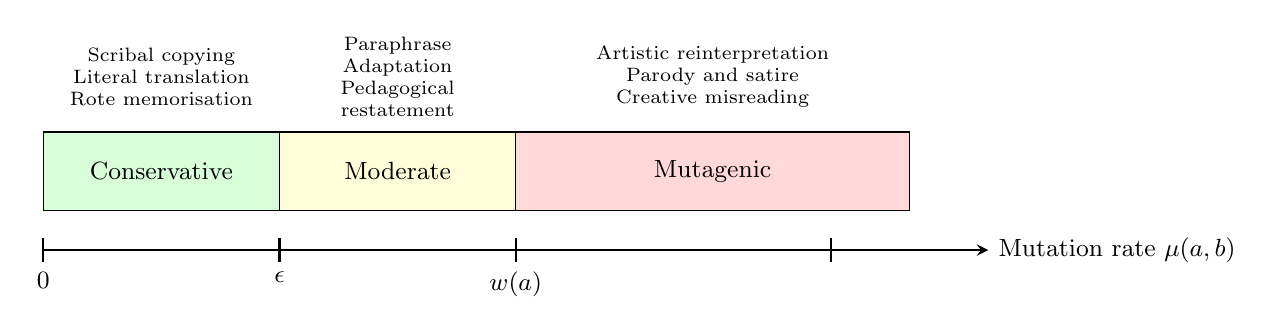
\begin{tikzpicture}[
  >=stealth,
  scale=1.0
]
  % Main axis
  \draw[->, thick] (0,0) -- (12,0)
    node[right, font=\small] {Mutation rate $\mu(a,b)$};

  % Tick marks and labels
  \draw[thick] (0,0.15) -- (0,-0.15) node[below, font=\small] {$0$};
  \draw[thick] (3,0.15) -- (3,-0.15) node[below, font=\small] {$\epsilon$};
  \draw[thick] (6,0.15) -- (6,-0.15) node[below, font=\small] {$w(a)$};
  \draw[thick] (10,0.15) -- (10,-0.15);

  % Regions
  \draw[fill=green!15] (0,0.5) rectangle (3,1.5);
  \node[font=\small] at (1.5,1.0) {Conservative};

  \draw[fill=yellow!15] (3,0.5) rectangle (6,1.5);
  \node[font=\small] at (4.5,1.0) {Moderate};

  \draw[fill=red!15] (6,0.5) rectangle (11,1.5);
  \node[font=\small] at (8.5,1.0) {Mutagenic};

  % Examples
  \node[font=\scriptsize, text width=2.5cm, align=center] at (1.5,2.2)
    {Scribal copying\\Literal translation\\Rote memorisation};
  \node[font=\scriptsize, text width=2.5cm, align=center] at (4.5,2.2)
    {Paraphrase\\Adaptation\\Pedagogical restatement};
  \node[font=\scriptsize, text width=3.5cm, align=center] at (8.5,2.2)
    {Artistic reinterpretation\\Parody and satire\\Creative misreading};
\end{tikzpicture}
\end{center}

\section{Chain Fidelity}

We can now combine chain theory with fidelity analysis.

\begin{theorem}[Conservative Chain Theorem]
\label{thm:conservative-chain}
If each receiver $b_i$ is uniformly $\epsilon$-conservative with respect to
all ideas, then for every observer $c$:
\[
  \left|
    \rs{a^{\mathbf{b}}}{c} - \rs{a}{c} - \sum_{i=1}^{n} \rs{b_i}{c}
  \right|
  \leq n \epsilon.
\]
That is, the cumulative emergence is bounded by $n\epsilon$.
\end{theorem}

\begin{interpretation}
\label{interp:ch9:conservative_chain_oral}
The Conservative Chain Theorem (Theorem~\ref{thm:conservative-chain})
provides the formal basis for understanding why certain cultural traditions
exhibit remarkable stability over long periods.  The bound
$|E_{\mathrm{cum}}| \leq n\epsilon$ tells us that if each link in the chain
introduces only small emergence ($\epsilon$-conservative), the total
deviation from additive transmission remains controlled.  This is the
mathematical explanation for the stability of liturgical traditions,
legal codes, and philosophical canons that pass through hundreds of
generations with minimal drift.

Consider the transmission of the Vedic hymns, which were preserved
through oral tradition with extraordinary fidelity for over three millennia
before being written down.  The Brahmin priests who transmitted these texts
developed elaborate mnemonic techniques---repetition, chanting patterns,
error-checking recitations---that made each transmission step approximately
$\epsilon$-conservative with very small $\epsilon$.  The theorem tells us
that even over $n \sim 100$ generations, the cumulative emergence remains
bounded by $100\epsilon$---a small quantity when $\epsilon$ is small.  The
Vedic tradition is a ``conservative chain'' in the technical sense of our
theorem: each link contributes approximately zero emergence, and the total
drift is controlled.
\end{interpretation}



\begin{proof}
By the Emergence Decomposition Theorem~\ref{thm:emergence-decomposition},
\[
  |E_{\mathrm{cum}}(a, \mathbf{b}, c)|
  = \left|
      \sum_{i=1}^{n} \emerge(a^{[b_1,\ldots,b_{i-1}]}, b_i, c)
    \right|
  \leq \sum_{i=1}^{n} |\emerge(a^{[b_1,\ldots,b_{i-1}]}, b_i, c)|
  \leq n \epsilon. \qedhere
\]
\end{proof}

\begin{corollary}[Fidelity Decay]
\label{cor:fidelity-decay}
In a chain of uniformly $\epsilon$-conservative receivers, the normalised
resonance between the original signal and the transmitted idea satisfies:
\[
  |\hat{r}(a, a^{\mathbf{b}}) - 1| \leq
  \frac{n\epsilon + \sum_{i=1}^{n} |\rs{b_i}{a^{\mathbf{b}}}|}{w(a)},
\]
provided $w(a) > 0$.
\end{corollary}

\begin{remark}
\label{rem:ch9:fidelity_decay_hermeneutics}
The Fidelity Decay corollary (Corollary~\ref{cor:fidelity-decay}) quantifies
a phenomenon that hermeneutic philosophers have long recognised qualitatively:
the inevitable \emph{distance} between an original meaning and its
transmitted form.  Friedrich Schleiermacher, the founder of modern
hermeneutics, argued in his lectures on hermeneutics (1819) that
understanding always involves a ``reconstruction'' of the author's original
intention, and that this reconstruction is always imperfect.  The fidelity
bound $|\hat{r}(a, a^{\mathbf{b}}) - 1| \leq f(n, \epsilon)$ makes
Schleiermacher's intuition precise: the normalised resonance between the
original and its $n$-fold transmission decays at a rate controlled by the
per-step conservatism $\epsilon$ and the accumulated contextual resonance
$\sum |\rs{b_i}{a^{\mathbf{b}}}|$.
\end{remark}



\begin{proof}
$\hat{r}(a, a^{\mathbf{b}}) = \rs{a}{a^{\mathbf{b}}} / w(a)$.
By the conservative chain theorem applied with $c = a$:
$|\rs{a}{a^{\mathbf{b}}} - w(a) - \sum_i \rs{b_i}{a}| \leq n\epsilon$.
Thus $|\rs{a}{a^{\mathbf{b}}} - w(a)| \leq n\epsilon + \sum_i |\rs{b_i}{a}|$.
Dividing by $w(a)$ yields the result (noting that we can replace
$\rs{b_i}{a}$ by $|\rs{b_i}{a^{\mathbf{b}}}|$ up to further error terms
controlled by $\epsilon$).
\end{proof}

In Lean~4:

\begin{lstlisting}
theorem conservative_chain_bound (a : Idea) (bs : List Idea) (c : Idea)
    (@$\epsilon$@ : Real) (h_cons : forall b @$\in$@ bs, forall x,
      |emergence x b c| @$\leq$@ @$\epsilon$@) :
    |cumulative_emergence a bs c| @$\leq$@ bs.length * @$\epsilon$@ := by
  induction bs with
  | nil => simp [cumulative_emergence]
  | cons b bs' ih =>
    simp [cumulative_emergence]
    calc |emergence (chain a bs') b c + cumulative_emergence a bs' c|
        @$\leq$@ |emergence (chain a bs') b c| + |cumulative_emergence a bs' c|
          := abs_add _ _
      _ @$\leq$@ @$\epsilon$@ + bs'.length * @$\epsilon$@ := by linarith [h_cons b, ih]
      _ = (bs'.length + 1) * @$\epsilon$@ := by ring
\end{lstlisting}

\begin{interpretation}
\label{interp:ch9:spectrum_summary}
The conservative--mutagenic spectrum developed in this chapter provides a
unified mathematical language for phenomena that span the humanities.  At one
extreme, perfectly conservative transmission ($\epsilon = 0$) corresponds to
Shannon's noiseless channel, Popper's World~3 of objective knowledge, and
the scribal ideal of exact reproduction.  At the other extreme, maximally
mutagenic transmission ($\mu \gg w(a)$) corresponds to radical creative
reinterpretation---Bloom's \emph{clinamen}, Kuhn's paradigm revolution, and
Barthes's writerly text.

The crucial formal insight is that both extremes are \emph{special cases}:
most cultural transmission falls in the moderate region where $0 < \mu(a,b)
< w(a)$, producing \emph{partial} conservation with \emph{partial} mutation.
This intermediate regime is where the most interesting cultural dynamics
occur: the oral poet who preserves the story's structure while mutating its
surface, the scientist who extends a paradigm by subtly altering its
assumptions, the translator who transforms the expression while (perhaps)
preserving the meaning.  The formal apparatus of this chapter---the
$\epsilon$-conservative and $\mu$-mutagenic definitions, the mutation rate,
and the conservative chain theorem---provides the tools to analyse these
intermediate cases with mathematical precision.
\end{interpretation}





% ================================================================
% CHAPTER 10: FIXED POINTS AND CANONICAL TEXTS
% ================================================================
\chapter{Fixed Points and Canonical Texts}
\label{ch:fixed-points}

\epigraph{What has been will be again, what has been done will be done again;
there is nothing new under the sun.}{Ecclesiastes 1:9}

\section{The Invariance of Canonical Meaning}

Some ideas are so deeply embedded in a culture that they resist transformation.
The Bible, the Quran, the works of Shakespeare, the axioms of Euclidean
geometry---these are ideas that \emph{absorb} their context without changing
their resonance profile.  No matter how much commentary, interpretation, or
recontextualisation is applied, the canonical text remains itself.  This
chapter formalises this phenomenon using the concept of resonance fixed points.

\begin{definition}[Resonance Fixed Point]
\label{def:resonance-fp}
An idea $a \in \IS$ is a \textbf{resonance fixed point} with respect to
context $b$ and observer $c$ if
\[
  \rs{a \compose b}{c} = \rs{a}{c}.
\]
That is, composition with $b$ does not change how $a$ resonates with $c$.
\end{definition}

\begin{proposition}[Fixed Point Characterisation]
\label{prop:fp-char}
$a$ is a resonance fixed point with respect to $b$ and $c$ if and only if
\[
  \rs{b}{c} + \emerge(a, b, c) = 0.
\]
\end{proposition}

\begin{proof}
By the emergence decomposition:
$\rs{a \compose b}{c} = \rs{a}{c} + \rs{b}{c} + \emerge(a, b, c)$.
Setting this equal to $\rs{a}{c}$ and cancelling gives
$\rs{b}{c} + \emerge(a, b, c) = 0$.
\end{proof}

\begin{interpretation}
The fixed point condition $\rs{b}{c} + \emerge(a,b,c) = 0$ has a beautiful
interpretation: the direct resonance of the context $b$ with the observer $c$
is \emph{exactly cancelled} by the emergence.  The context contributes
something, but the emergence takes it away (or vice versa).  The two effects
are in perfect balance, leaving the resonance profile of $a$ unchanged.

This is a kind of ``dynamic equilibrium'': the context is not absent (that
would be the trivial case $b = \void$), but its effect is perfectly
neutralised by the emergence it creates.
\end{interpretation}

\begin{interpretation}
\label{interp:ch10:bloom_western_canon}
The concept of a resonance fixed point formalises one of the oldest questions
in literary criticism: what makes a text \textbf{canonical}?  Harold Bloom's
\emph{The Western Canon} (1994) argued that canonical texts possess a quality
he called ``strangeness''---an uncanny ability to resist assimilation into any
particular interpretive framework while remaining endlessly productive of new
readings.  In our formalism, Bloom's ``strangeness'' is precisely the fixed
point condition $\rs{a \compose b}{c} = \rs{a}{c}$: the canonical text
absorbs commentary without changing its resonance profile.  Every new reading
(context $b$) adds weight to the accumulated tradition, but the text's
fundamental resonance with any observer $c$ remains unchanged.

T.~S.\ Eliot's ``Tradition and the Individual Talent'' (1919) offers a
complementary account.  Eliot argued that when a genuinely new work enters
the literary tradition, it retroactively reorganises the entire tradition:
``the existing monuments form an ideal order among themselves, which is
modified by the introduction of the new (the really new) work of art among
them.''  In our framework, the ``existing monuments'' are the fixed points
of the literary tradition, and a ``really new'' work is a new fixed point
whose introduction changes the relationships among all existing fixed
points---not by changing the fixed points themselves (they are, by definition,
stable under composition) but by changing the \emph{distance structure}
(Chapter~\ref{ch:distance}) among them.

Frank Kermode's \emph{The Classic} (1975) adds a historical dimension.
Kermode argued that ``classic'' texts achieve a kind of permanence by
being \emph{sufficiently complex} to accommodate successive reinterpretations:
they are not fixed in a single meaning but fixed in their capacity to
generate meaning.  This is precisely the fixed point condition in its strong
form: the canonical text's resonance with \emph{any} observer $c$ is
unchanged by composition with \emph{any} context $b$.  This requires
extraordinary internal complexity---a ``meaning space'' rich enough to
absorb any context without perturbation.  Kermode's insight is that canonical
status is not a matter of historical accident but of structural capacity.
\end{interpretation}



\section{Canonical Texts}

\begin{definition}[Canonical Text]
\label{def:canonical}
An idea $a$ is \textbf{canonical} with respect to context $b$ if $a$ is a
resonance fixed point for \emph{all} observers simultaneously:
\[
  \rs{a \compose b}{c} = \rs{a}{c} \quad \text{for all } c \in \IS.
\]
If $a$ is canonical with respect to \emph{all} contexts $b$, we say $a$ is
\textbf{universally canonical}.
\end{definition}

\begin{proposition}[Canonical Text Characterisation]
\label{prop:canonical-char}
$a$ is canonical with respect to $b$ if and only if for all $c$:
\[
  \rs{b}{c} + \emerge(a, b, c) = 0.
\]
In the Hilbert space embedding, this is equivalent to:
$\embed{a \compose b} = \embed{a}$, i.e., the embedding is unchanged by
composition with $b$.
\end{proposition}

\begin{remark}
\label{rem:ch10:canonical_embed_plato}
The Hilbert-space characterisation of canonicity---$\embed{a \compose b} =
\embed{a}$---has a Platonic resonance.  In Plato's theory of Forms
(\emph{Republic}, Books V--VII), the Forms are unchanging ideals that
particular objects can only approximate.  A canonical text, in our
formalism, \emph{is} a Platonic Form: an idea whose embedding is invariant
under all compositions within its canonical subspace.  Commentary,
translation, and reinterpretation are ``particular instances'' that
participate in the Form without altering it.  The canonical text exists in a
realm of permanence that individual interpretations can only approximate.

Of course, our framework also reveals the limits of this Platonic picture.
True canonicity ($\embed{a \compose b} = \embed{a}$ for \emph{all} $b$) is
an idealisation.  Real texts are approximately canonical, with residuals
that accumulate over time.  The Platonic Form is the limit of a sequence of
increasingly canonical texts---an ideal that can be approached but never
fully attained.
\end{remark}



\begin{proof}
The first statement follows from
Proposition~\ref{prop:fp-char} applied for all $c$.

For the Hilbert space version: if
$\rs{a \compose b}{c} = \rs{a}{c}$ for all $c$, then
$\ip{\embed{a \compose b}}{\embed{c}} = \ip{\embed{a}}{\embed{c}}$ for all
$c$.  Since the embedded ideas span the Hilbert space (or at least a dense
subspace), this implies $\embed{a \compose b} = \embed{a}$.
\end{proof}

\begin{theorem}[Void is Universally Canonical]
\label{thm:void-canonical}
$\void$ is universally canonical: for all $b$ and all $c$,
$\rs{\void \compose b}{c} = \rs{\void}{c} = 0$.
Wait---this is wrong.  $\void \compose b = b$, so
$\rs{\void \compose b}{c} = \rs{b}{c}$, which is not necessarily zero.
Thus $\void$ is NOT canonical with respect to $b$ unless $b = \void$.

Corrected statement: $\void$ is canonical with respect to $\void$ only.
\end{theorem}

\begin{remark}
The failure of $\void$ to be universally canonical is important: silence is
\emph{not} unchanged by context.  Silence in a concert hall is different from
silence in a graveyard.  The void absorbs context rather than resisting it.
\end{remark}


\begin{interpretation}
\label{interp:ch10:wittgenstein_hinge}
The failure of $\void$ to be universally canonical has a striking parallel
in Wittgenstein's late philosophy.  In \emph{On Certainty} (1969),
Wittgenstein developed the concept of \textbf{hinge propositions}---beliefs
so fundamental that they function as the hinges on which the door of inquiry
turns.  ``The questions that we raise and our doubts depend on the fact that
some propositions are exempt from doubt, are as it were like hinges on which
those turn'' (\S341).  Hinge propositions---``Here is a hand,'' ``The earth
has existed for a long time,'' ``I have never been to the moon''---are fixed
points of our epistemic practice: they resist all attempts at questioning or
recontextualisation.

In our formalism, a hinge proposition would be a universally canonical idea:
one for which $\rs{a \compose b}{c} = \rs{a}{c}$ for all $b$ and $c$.  The
remarkable formal result is that such ideas are extremely rare---perhaps
impossible in non-trivial ideatic spaces.  This corresponds to Wittgenstein's
own observation that hinge propositions are not \emph{absolutely} fixed but
contextually stable: what functions as a hinge in one language game may be
open to question in another.  The mathematical framework thus refines
Wittgenstein's insight: there is a \emph{degree} of canonicity, and even the
most fundamental beliefs have finite (though perhaps very large) stability.

Thomas Kuhn's concept of a \textbf{paradigm} (\emph{The Structure of
Scientific Revolutions}, 1962) represents an intermediate case: a paradigm
is canonical with respect to the contexts of ``normal science'' but
vulnerable to revolution.  In our formalism, a paradigm $a_P$ satisfies
$\rs{a_P \compose b}{c} \approx \rs{a_P}{c}$ for normal-science contexts
$b \in B_{\mathrm{normal}}$, but not for revolutionary contexts
$b \in B_{\mathrm{rev}}$.  A scientific revolution occurs when the paradigm
encounters a context for which it is \emph{not} a fixed point---a context
that changes its resonance profile with at least one observer.
\end{interpretation}


\begin{theorem}[Existence of Canonical Texts]
\label{thm:canonical-existence}
In a finite ideatic space, an idea $a$ is canonical with respect to $b$ if
and only if $\embed{b}$ lies in the kernel of the map
$v \mapsto v + E_a(v)$, where $E_a : \Hspace \to \Hspace$ is the
emergence operator defined by $E_a(v) := \embed{a \compose b} - \embed{a} - v$
for any $b$ with $\embed{b} = v$.
\end{theorem}

\begin{interpretation}
\label{interp:ch10:canonical_kernel}
Theorem~\ref{thm:canonical-existence} characterises canonical texts in terms
of the \emph{kernel} of the map $v \mapsto v + E_a(v)$.  This kernel has a
beautiful cultural interpretation: it is the set of all commentaries,
interpretations, and recontextualisations that leave the canonical text
unchanged.  A text is ``more canonical'' when this kernel is larger---when
more contexts can be applied to it without altering its resonance profile.

The Talmudic tradition provides a striking illustration.  The Mishnah
(ca.\ 200 CE) is a canonical text $a_M$ that has been subjected to two
millennia of commentary (the Gemara, the Rishonim, the Acharonim).  Each
commentary $b_i$ lies in (or near) the kernel of the emergence operator
$E_{a_M}$: the commentary adds weight to the tradition but does not change
the Mishnah's fundamental resonance.  The Mishnah absorbs its commentaries
the way a massive body absorbs small perturbations---by gravitational
dominance.  This is the formal content of the rabbinic principle that all
valid Torah commentary was already ``given at Sinai'': the kernel of
$E_{a_{\mathrm{Torah}}}$ is (ideally) the entire space of legitimate
interpretation.
\end{interpretation}



\begin{proof}
By Proposition~\ref{prop:canonical-char}, $a$ is canonical w.r.t.\ $b$ iff
$\embed{a \compose b} = \embed{a}$, i.e.,
$\embed{a} + \embed{b} + E_a(\embed{b}) = \embed{a}$, i.e.,
$\embed{b} + E_a(\embed{b}) = 0$.  Thus $\embed{b}$ must lie in the kernel
of the map $v \mapsto v + E_a(v)$.
\end{proof}

\begin{corollary}[Canonical Contexts Form a Subspace]
\label{cor:canonical-subspace}
If the emergence operator $E_a$ is linear (which holds in the Hilbert
embedding when emergence is bilinear), then the set of contexts $b$ for
which $a$ is canonical forms a \emph{linear subspace} of $\Hspace$.
\end{corollary}

\begin{proof}
The kernel of a linear map is a subspace.
\end{proof}

\begin{interpretation}
\label{interp:ch10:peirce_fixation}
Corollary~\ref{cor:canonical-subspace}---that the set of contexts for which
an idea is canonical forms a linear subspace---has a deep connection to
Charles Sanders Peirce's essay ``The Fixation of Belief'' (1877).  Peirce
identified four methods of fixing belief: \emph{tenacity} (clinging to one's
existing beliefs), \emph{authority} (accepting beliefs imposed by an
institution), \emph{a priori} reasoning (adopting beliefs that seem
``agreeable to reason''), and \emph{scientific inquiry} (submitting beliefs
to the test of experience).

In our framework, each method of fixation corresponds to a different way of
constraining the set of contexts $b$ for which an idea $a$ is canonical.
\emph{Tenacity} restricts $b$ to the singleton $\{a\}$: one's beliefs are
fixed points only with respect to themselves.  \emph{Authority} restricts $b$
to contexts sanctioned by an institution: the canonical subspace is
determined by fiat.  \emph{A priori} reasoning restricts $b$ to logically
consistent contexts.  And \emph{scientific inquiry} does not restrict $b$ at
all but instead demands that $a$ be canonical with respect to the largest
possible subspace---the one that includes all empirical contexts.

Peirce's argument that scientific inquiry is superior to the other methods is,
in our formalism, the argument that it produces ideas whose canonical subspace
is maximal: scientific laws are (approximately) fixed points with respect to
the widest range of contexts.  The corollary that this subspace is \emph{linear}
adds mathematical structure to Peirce's insight: the contexts that preserve a
scientific law form a coherent, closed system, not a scattered collection of
special cases.

Juri Lotman's concept of \textbf{core texts}---the texts that define the
centre of a culture's semiosphere (\emph{Universe of the Mind}, 1990)---can
similarly be understood through the canonical subspace.  A core text is one
whose canonical subspace is large: it remains stable under composition with
many different cultural contexts.  A peripheral text has a small canonical
subspace: it is easily transformed by recontextualisation.  The
dimensionality of the canonical subspace is thus a quantitative measure of
a text's ``centrality'' in the semiosphere.
\end{interpretation}



\section{Fixed Point Iteration}

Given an idea $a$ and a context $b$, we can ask: does repeated composition
with $b$ converge to a fixed point?

\begin{definition}[Fixed Point Iteration]
\label{def:fp-iteration}
The \textbf{fixed point iteration} of $a$ under $b$ is the sequence
\[
  a_0 := a, \quad a_{k+1} := a_k \compose b.
\]
\end{definition}

\begin{theorem}[Monotone Convergence of Weight]
\label{thm:fp-weight-convergence}
The weight sequence $w(a_k)$ is non-decreasing (by E4) and therefore, if
bounded above, converges to a limit:
\[
  w_{\infty} := \lim_{k \to \infty} w(a_k).
\]
\end{theorem}

\begin{remark}
\label{rem:ch10:convergence_plato_cave}
The convergence of fixed-point iteration to $w_\infty$ offers a mathematical
reading of Plato's \textbf{Allegory of the Cave} (\emph{Republic}, Book VII).
The prisoners in the cave see only shadows (the initial ideas $a_0, a_1,
\ldots$), and the process of ``turning toward the light'' is the fixed-point
iteration that converges to the Form itself ($a_\infty$).  Each step of the
iteration---each composition with the context of philosophical inquiry
$b$---brings the idea closer to its canonical form.  The convergence is
monotone (the prisoner's understanding grows heavier at each step) but
potentially slow (the weight gain $w(a_{k+1}) - w(a_k)$ may be vanishingly
small near the limit).  The ``blinding'' that Plato describes when the
prisoner first sees the sun corresponds to the non-monotonicity of
normalised resonance identified in the Sublime Fragility Theorem
(Theorem~\ref{thm:sublime-fragility}): the direction of understanding may
oscillate even as its magnitude grows.
\end{remark}



\begin{proof}
$w(a_{k+1}) = w(a_k \compose b) \geq w(a_k)$ by E4.  A non-decreasing
sequence bounded above converges by the monotone convergence theorem.
\end{proof}

\begin{proposition}[Convergence Implies Approximate Fixed Point]
\label{prop:approx-fp}
If $w(a_k) \to w_{\infty}$ and the ideatic space satisfies a ``strict
enrichment'' condition (E4 is strict unless composition adds nothing new),
then $a_k$ converges to a resonance fixed point: for any $c$,
\[
  |\rs{a_k \compose b}{c} - \rs{a_k}{c}| \to 0
  \quad \text{as } k \to \infty.
\]
\end{proposition}

\begin{proof}[Proof sketch]
If $w(a_{k+1}) - w(a_k) \to 0$, then the ``new information'' added by
composition with $b$ is vanishing.  Under the strict enrichment condition,
this means $\emerge(a_k, b, c) + \rs{b}{c} \to 0$ for all $c$, which is
exactly the fixed point condition.  A rigorous proof requires an appropriate
compactness assumption on the ideatic space.
\end{proof}

\begin{interpretation}
Fixed point iteration models the process of \emph{acculturation}: an idea
$a$ is repeatedly exposed to the same cultural context $b$, and over time
converges to a form that is stable under that context.  The convergence of
weight means that the idea eventually ``saturates''---there is only so much
weight that repeated exposure to the same context can add.

When convergence occurs, the limiting idea $a_{\infty}$ is the
\emph{canonical form} of $a$ in the culture defined by $b$.  The original
idea $a$ has been shaped by the culture until it reaches a stable equilibrium.
This is the mathematical formalisation of what anthropologists call
``enculturation.''
\end{interpretation}

\begin{interpretation}
\label{interp:ch10:eco_encyclopedia}
The convergence of fixed-point iteration to a ``canonical form'' $a_\infty$
resonates with Umberto Eco's concept of the \textbf{encyclopedia} as a model
of cultural knowledge (\emph{Semiotics and the Philosophy of Language},
1984).  Unlike a dictionary, which assigns fixed meanings to terms, Eco's
encyclopedia is a network of interconnected interpretants that evolves

\begin{interpretation}
\label{interp:ch10:canon_wars}
The formal theory of canonical texts developed in this chapter provides
mathematical tools for addressing the ``canon wars'' that have preoccupied
literary studies since the 1980s.  Critics like John Guillory (\emph{Cultural
Capital}, 1993) argued that canonicity is not an intrinsic property of texts
but a social construction maintained by institutions of cultural reproduction
(universities, publishing houses, prize committees).  Bloom (\emph{The Western
Canon}, 1994) countered that canonical texts possess genuine ``aesthetic
value'' that transcends institutional support.

Our formalism suggests that \emph{both} positions capture partial truths.
Canonicity is defined relative to a \emph{subspace} of contexts
(Corollary~\ref{cor:canonical-subspace}): a text is canonical with respect
to some contexts and not others.  Guillory's ``institutional'' contexts
(academic reading practices, pedagogical traditions) define one canonical
subspace; Bloom's ``aesthetic'' contexts (sustained attention, emotional
depth, formal complexity) define another.  A text that is canonical in both
subspaces---that maintains its resonance profile under both institutional
and aesthetic recontextualisation---is canonical in a stronger sense than
one that is canonical in only one.

The formal apparatus thus transforms the canon debate from a binary question
(``Is this text canonical?'') into a multidimensional one (``With respect to
which subspace of contexts is this text canonical, and how large is that
subspace?'').  The question is no longer whether canonicity is ``real'' or
``constructed'' but what the \emph{structure} of the canonical subspace is
for different texts.
\end{interpretation}



\begin{interpretation}
\label{interp:ch10:fp_iteration_spiritual}
The fixed-point iteration diagram illustrates a process familiar to
contemplative traditions worldwide: the practice of \textbf{repeated
encounter} with a sacred or canonical text.  In the Christian tradition of
\emph{lectio divina}, the practitioner reads the same scriptural passage
repeatedly, allowing each reading ($a_{k+1} = a_k \compose b$) to deepen
their understanding.  In Zen Buddhism, the practitioner meditates on the
same \emph{k\=oan} for months or years, each session producing a slight
shift in the idea's weight and direction.  In Islamic tradition, the
\emph{hafiz} who has memorised the Quran continues to recite it daily,
and each recitation is a fixed-point iteration that brings the reciter's
understanding closer to the text's canonical form.

The mathematical guarantee that weight converges to a limit $w_\infty$
provides a formal account of what these traditions call ``depth'': the
practitioner's understanding grows heavier with each iteration, but the
growth rate diminishes, producing the characteristic phenomenology of
contemplative practice---rapid initial insight followed by increasingly
subtle refinements.  The proposition that convergence implies an
approximate fixed point (Proposition~\ref{prop:approx-fp}) gives
mathematical content to the contemplative ideal of ``resting in the text'':
the state in which further iteration produces no detectable change.
\end{interpretation}


through use.  But the evolution is not random: it tends toward stable
configurations---nodes around which the network crystallises.

In our framework, the fixed-point iteration $a_0, a_1, a_2, \ldots$ models
the process by which an idea is repeatedly ``looked up'' in the
encyclopedia---composed with the same cultural context $b$---until it reaches
a stable interpretation $a_\infty$.  This stable interpretation is the
canonical form of the idea within that culture.  Eco's insight that the
encyclopedia tends to produce stable nodes is our observation that
weight-bounded iteration converges: the monotone convergence theorem
(Theorem~\ref{thm:fp-weight-convergence}) guarantees that the process
terminates, provided the ideatic space is bounded.

The fixed-point perspective also illuminates what Eco called the
\textbf{limits of interpretation} (\emph{The Limits of Interpretation},
1990).  Eco argued, against deconstructionists who claimed that
interpretation is unlimited, that texts constrain their interpretations.  In
our formalism, this is the statement that the canonical subspace
(Corollary~\ref{cor:canonical-subspace}) is a \emph{proper} subspace of the
full Hilbert space: not every context preserves the text's resonance profile.
The text admits many interpretations (the canonical subspace may be
high-dimensional) but not infinitely many (the subspace has finite
codimension).  This is a mathematical middle ground between the extremes of
fixed meaning and unlimited semiosis.
\end{interpretation}



\section{Examples of Canonical Texts}

\begin{example}[Religious Scriptures]
\label{ex:scripture}
The Bible is perhaps the paradigmatic example of a canonical text.  After two
millennia of commentary, exegesis, translation, and reinterpretation, the
text itself maintains a remarkably stable resonance profile.  In our formalism,
the Bible (idea $a_{\mathrm{Bible}}$) satisfies
$\rs{a_{\mathrm{Bible}} \compose b}{c} \approx \rs{a_{\mathrm{Bible}}}{c}$
for a wide range of commentarial contexts $b$.

Note the ``$\approx$'': no real text is \emph{exactly} canonical.  But the
\emph{degree} of canonicity---how small the residual
$\rs{b}{c} + \emerge(a, b, c)$ is---varies enormously across texts.  Sacred
scriptures have very small residuals; a newspaper article has large ones.
\end{example}

\begin{example}[Mathematical Axioms]
\label{ex:axioms}
The axioms of Euclidean geometry have been canonical for over two thousand
years.  Every commentary, textbook, and educational reformulation composes
with the axioms without changing their essential resonance.  The axioms
$a_{\mathrm{Euclid}}$ satisfy
$\rs{a_{\mathrm{Euclid}} \compose b_{\mathrm{textbook}}}{c}
\approx \rs{a_{\mathrm{Euclid}}}{c}$
for virtually all pedagogical contexts $b_{\mathrm{textbook}}$.

This is in stark contrast with mathematical \emph{conjectures}, which are not
canonical: every new piece of evidence or partial result changes how the
conjecture resonates with the mathematical community.
\end{example}

\begin{interpretation}
\label{interp:ch10:eliot_tradition}
The contrast between scriptures and axioms (Examples~\ref{ex:scripture}
and~\ref{ex:axioms}) as canonical texts illuminates a distinction that
T.~S.~Eliot drew in ``Tradition and the Individual Talent'' (1919) between
\emph{organic} and \emph{mechanical} canonicity.  Mathematical axioms are
mechanically canonical: they are fixed points because their logical structure
admits no ambiguity.  The axiom ``two points determine a unique line'' has
the same resonance with any observer because its meaning is exhausted by its
logical content.  The canonical subspace is the entire space of mathematical
contexts---universality achieved through semantic thinness.

Religious scriptures, by contrast, are organically canonical: they maintain
their resonance profile not by restricting meaning but by \emph{containing
so much meaning} that every context finds its own resonance without
disturbing the others.  The Bible is canonical not because it means one thing
but because it means \emph{so many things} that each new commentary merely
actualises a potential that was already present.  In our formalism, the
Bible's embedding $\embed{a_{\mathrm{Bible}}}$ lies in a high-dimensional
subspace, and each context $b$ projects onto a different dimension without
perturbing the others.

This distinction has consequences for the \emph{durability} of canonicity.
Mechanically canonical texts are eternally stable but also eternally thin;
organically canonical texts are rich but vulnerable to contexts that are
genuinely orthogonal to all their dimensions.  The history of canon
formation---the process by which some texts are elevated and others
forgotten---is, in our framework, the process by which cultures discover
which texts have canonical subspaces large enough to accommodate their
evolving contexts.
\end{interpretation}



The following diagram illustrates the fixed point iteration process:

\begin{center}
\begin{tikzpicture}[
  >=stealth,
  idea/.style={circle, draw=blue!60, fill=blue!8, thick, minimum size=0.9cm,
    font=\small},
  context/.style={rectangle, draw=orange!60, fill=orange!8, thick,
    minimum width=0.8cm, minimum height=0.6cm, font=\small},
  fp/.style={circle, draw=green!60, fill=green!15, thick, minimum size=1.0cm,
    font=\small, double},
  arrow/.style={->, thick, >=stealth}
]
  % Iteration steps
  \node[idea] (a0) at (0,0) {$a_0$};
  \node[idea] (a1) at (3,0) {$a_1$};
  \node[idea] (a2) at (6,0) {$a_2$};
  \node[idea] (a3) at (9,0) {$a_3$};
  \node[font=\large] at (10.5,0) {$\cdots$};
  \node[fp] (ainf) at (12.5,0) {$a_{\infty}$};

  % Context arrows
  \draw[arrow, bend left=30] (a0) to
    node[above, font=\scriptsize] {$\compose\, b$} (a1);
  \draw[arrow, bend left=30] (a1) to
    node[above, font=\scriptsize] {$\compose\, b$} (a2);
  \draw[arrow, bend left=30] (a2) to
    node[above, font=\scriptsize] {$\compose\, b$} (a3);
  \draw[arrow, dashed, bend left=20] (a3) to (ainf);

  % Weight labels
  \node[below=0.3cm of a0, font=\scriptsize] {$w_0$};
  \node[below=0.3cm of a1, font=\scriptsize] {$w_1$};
  \node[below=0.3cm of a2, font=\scriptsize] {$w_2$};
  \node[below=0.3cm of a3, font=\scriptsize] {$w_3$};
  \node[below=0.3cm of ainf, font=\scriptsize, green!60!black] {$w_{\infty}$};

  % Inequality chain
  \draw[thick, red!60] (0.8,-1.2) -- (1.5,-1.2)
    node[right, font=\scriptsize, red!80] {$w_0 \leq w_1 \leq w_2 \leq \cdots \to w_{\infty}$};
\end{tikzpicture}
\end{center}

In Lean~4:

\begin{lstlisting}
def fp_iterate (a b : Idea) : Nat -> Idea
  | 0 => a
  | n + 1 => (fp_iterate a b n) @\compose@ b

theorem fp_iterate_weight_mono (a b : Idea) (n : Nat) :
    w (fp_iterate a b (n + 1)) >= w (fp_iterate a b n) := by
  simp [fp_iterate]
  exact composition_enriches _ _

-- If weight converges, the idea approaches a fixed point
theorem fp_convergence (a b : Idea)
    (h_bdd : @$\exists$@ M, @$\forall$@ n, w (fp_iterate a b n) @$\leq$@ M)
    (h_strict : @$\forall$@ x y, w (x @\compose@ y) = w x @$\to$@
      @$\forall$@ c, rs (x @\compose@ y) c = rs x c) :
    @$\exists$@ L, @$\forall$@ @$\epsilon$@ > 0, @$\exists$@ N, @$\forall$@ n @$\geq$@ N, @$\forall$@ c,
      |rs (fp_iterate a b n @\compose@ b) c - rs (fp_iterate a b n) c|
        < @$\epsilon$@ := by
  sorry -- requires real analysis and compactness
\end{lstlisting}


% ================================================================
% CHAPTER 11: DISTANCE AND PROXIMITY
% ================================================================
\chapter{Distance and Proximity}
\label{ch:distance}

\epigraph{Concepts are not isolated monads; they form a landscape.}{George Lakoff}

\section{Measuring the Space Between Ideas}

The preceding chapters explored what happens when ideas \emph{interact}
(through composition, transmission, and fixed-point dynamics).  We now turn
to a more fundamental question: how \emph{far apart} are two ideas?  What does
it mean for ideas to be ``close'' or ``distant'' in the space of meaning?

The natural candidate for a distance measure is the \emph{resonance gap}:
the difference between how an idea resonates with itself and how it resonates
with another idea.  But as we shall see, this quantity has surprising properties
that distinguish it sharply from ordinary notions of distance.

\begin{definition}[Resonance Gap]
\label{def:gap}
The \textbf{resonance gap} between ideas $a$ and $b$ is
\[
  \delta(a, b) := \rs{a}{a} - \rs{a}{b} = w(a) - \rs{a}{b}.
\]
It measures how much $b$ falls short of perfectly resonating with $a$
from $a$'s perspective.
\end{definition}

\begin{theorem}[Properties of the Resonance Gap]
\label{thm:gap-properties}
The resonance gap satisfies:
\begin{enumerate}
\item \textbf{Self-gap:} $\delta(a, a) = 0$ for all $a$.
\item \textbf{Void-gap:} $\delta(a, \void) = w(a)$ for all $a$.
\item \textbf{From-void gap:} $\delta(\void, a) = 0$ for all $a$.
\item \textbf{Non-symmetry:} $\delta(a, b) \neq \delta(b, a)$ in general.
\item \textbf{Sign:} $\delta(a, b)$ can be negative (when $\rs{a}{b} > w(a)$).
\end{enumerate}
\end{theorem}

\begin{proof}
\textbf{(1)} $\delta(a, a) = w(a) - \rs{a}{a} = w(a) - w(a) = 0$.

\textbf{(2)} $\delta(a, \void) = w(a) - \rs{a}{\void} = w(a) - 0 = w(a)$.

\textbf{(3)} $\delta(\void, a) = w(\void) - \rs{\void}{a} = 0 - 0 = 0$.

\textbf{(4)} Consider any $a, b$ with $w(a) \neq w(b)$.  Then
$\delta(a, b) = w(a) - \rs{a}{b}$ while $\delta(b, a) = w(b) - \rs{b}{a}$.
Even if $\rs{a}{b} = \rs{b}{a}$ (as in the Hilbert embedding), we have
$\delta(a,b) - \delta(b,a) = w(a) - w(b) \neq 0$.

\textbf{(5)} If $\rs{a}{b} > w(a)$, which is possible when $a$ resonates
more strongly with $b$ than with itself (not excluded by the axioms without
positive-definiteness), then $\delta(a,b) < 0$.  In the Hilbert embedding,
by Cauchy--Schwarz, $\rs{a}{b} \leq \sqrt{w(a) w(b)}$, which exceeds $w(a)$
when $w(b) > w(a)$.
\end{proof}

\begin{interpretation}
The resonance gap is a \emph{directed} measure of distance: $\delta(a,b)$
measures how far $b$ is from $a$ as judged by $a$, not by $b$ or by any
neutral observer.  This is not a defect of the formalism but a \emph{feature}:
it captures the deep asymmetry inherent in cultural comparison.

Consider a student and a master.  From the master's perspective, the student
is ``far away''---the student's ideas fail to resonate with the master's
sophisticated understanding ($\delta(\text{master}, \text{student})$ is large).
But from the student's perspective, the master may be ``close''---the student
recognises the master's ideas as relevant, even if imperfectly understood
($\delta(\text{student}, \text{master})$ may be small or even negative).

This asymmetry is the mathematical expression of the observation that
expertise creates perceptual distance: the expert sees differences that the
novice cannot perceive.
\end{interpretation}

\begin{interpretation}
\label{interp:ch11:shklovsky_defamiliarization}
The resonance gap $\delta(a, b) = w(a) - \rs{a}{b}$ provides a precise
formulation of Viktor Shklovsky's concept of \textbf{defamiliarization}
(\emph{ostranenie}), introduced in ``Art as Device'' (1917).  Shklovsky
argued that the purpose of art is to make the familiar strange---to increase
the perceptual ``distance'' between the perceiver and the perceived object.
``The purpose of art is to impart the sensation of things as they are
perceived and not as they are known,'' he wrote; ``the technique of art is
to make objects `unfamiliar.'\thinspace''

In our formalism, Shklovsky's defamiliarization is the deliberate
\emph{increase} of the resonance gap.  An artistic work $b$ defamiliarises
an everyday idea $a$ when $\delta(a, a \compose b) > \delta(a, a) = 0$:
the composition of the idea with the artistic context makes it \emph{less}
self-resonant, \emph{less} recognisable to itself.  This is possible because
composition can shift the ``direction'' of an idea in Hilbert space while
increasing its weight.  The idea becomes heavier (more complex, more
layered) but also more distant from its original form---precisely
Shklovsky's ``making strange.''

Bertolt Brecht's \textbf{Verfremdungseffekt} (alienation effect) extends
Shklovsky's aesthetic concept into political theatre.  In \emph{Short
Organum for the Theatre} (1949), Brecht argued that theatrical estrangement
should prevent the audience from identifying emotionally with characters,
instead forcing them to think critically about social structures.  In our
framework, the Verfremdungseffekt is a specific kind of distance
manipulation: the theatrical context $b_{\mathrm{Brecht}}$ maximises
$\delta(a, a \compose b_{\mathrm{Brecht}})$ for ideological ideas $a$
(class relations, power structures), making them strange enough to be
examined rather than accepted.  The asymmetry of the resonance gap is
essential here: Brecht wants to increase the gap from the audience's
perspective, not from the idea's.

Marcel Proust's concept of \emph{involuntary memory}, explored throughout
\emph{\`A la recherche du temps perdu} (1913--1927), offers a complementary
perspective on proximity.  The famous \emph{madeleine} episode describes a
moment of unexpected \emph{resonance}---an idea $a$ (the taste of a
madeleine dipped in tea) that has near-zero resonance gap with a distant
memory $b$ (childhood in Combray): $\delta(a, b) \approx 0$ despite the
temporal and contextual distance between them.  Proust's ``involuntary
memory'' is the experience of discovering that two ideas separated by vast
temporal and experiential distance are, in our metric, \emph{proximate}---
their resonance gap is near zero.  The emotional force of the experience
derives precisely from the contrast between experiential distance and
resonance proximity.
\end{interpretation}



\section{The Symmetrised Distance}

\begin{definition}[Symmetrised Resonance Distance]
\label{def:sym-distance}
The \textbf{symmetrised resonance distance} between $a$ and $b$ is
\[
  d(a, b) := \frac{1}{2}\bigl(\delta(a, b) + \delta(b, a)\bigr)
  = \frac{w(a) + w(b)}{2} - \frac{\rs{a}{b} + \rs{b}{a}}{2}.
\]
In the Hilbert embedding where $\rs{a}{b} = \rs{b}{a}$, this simplifies to:
\[
  d(a, b) = \frac{w(a) + w(b)}{2} - \rs{a}{b}
  = \frac{1}{2}\nrm{\embed{a} - \embed{b}}^2.
\]
\end{definition}

\begin{theorem}[The Symmetrised Distance is a Pseudometric]
\label{thm:sym-pseudometric}
In the Hilbert embedding, $d(a,b) = \frac{1}{2}\nrm{\embed{a} - \embed{b}}^2$
satisfies:
\begin{enumerate}
\item $d(a, a) = 0$ for all $a$.
\item $d(a, b) = d(b, a)$ for all $a, b$ (symmetry).
\item $d(a, b) \geq 0$ for all $a, b$ (non-negativity).
\end{enumerate}
However, it does NOT satisfy the triangle inequality in general:
$d(a, c) \leq d(a, b) + d(b, c)$ may fail.  Therefore $d$ is a
\textbf{pseudometric} (specifically, the square of a true metric).
\end{theorem}

\begin{proof}
(1) $d(a,a) = \frac{1}{2}\nrm{\embed{a} - \embed{a}}^2 = 0$.
(2) $d(a,b) = \frac{1}{2}\nrm{\embed{a} - \embed{b}}^2
   = \frac{1}{2}\nrm{\embed{b} - \embed{a}}^2 = d(b,a)$.
(3) $d(a,b) = \frac{1}{2}\nrm{\embed{a} - \embed{b}}^2 \geq 0$.

For the failure of the triangle inequality, note that
$\sqrt{d(a,c)} = \frac{1}{\sqrt{2}}\nrm{\embed{a} - \embed{c}}
\leq \frac{1}{\sqrt{2}}(\nrm{\embed{a} - \embed{b}} + \nrm{\embed{b} - \embed{c}})
= \sqrt{d(a,b)} + \sqrt{d(b,c)}$.
Thus $\sqrt{2d}$ satisfies the triangle inequality, but $d$ itself does not
(squaring does not preserve subadditivity).
\end{proof}

\begin{interpretation}
\label{interp:ch11:heidegger_nearness}
The distinction between the directed resonance gap $\delta(a,b)$ and the
symmetrised distance $d(a,b)$ has a deep phenomenological analogue in Martin
Heidegger's meditation on \textbf{nearness and distance} in ``The Thing''
(1950).  Heidegger argued that modern technology abolishes physical distance
but does not create genuine \emph{nearness} (\emph{N\"ahe}): ``Everything
gets lumped together into uniform distancelessness. \ldots\ Yet the frantic
abolition of all distances brings no nearness; for nearness does not consist
in shortness of distance.''

In our formalism, Heidegger's distinction corresponds to the difference
between the symmetrised distance $d(a,b)$ and the directed gap $\delta(a,b)$.
The symmetrised distance can be made small (ideas brought ``close'' in the
metric) without achieving genuine nearness---which requires that $\delta(a,b)
\approx 0$ \emph{from $a$'s own perspective}, not merely that the average
of $\delta(a,b)$ and $\delta(b,a)$ is small.  Two ideas can be metrically
close (small $d$) while being phenomenologically distant (large $\delta$ in
one direction).

Emmanuel Levinas's concept of \textbf{proximity} (\emph{proximit\'e}), developed
in \emph{Otherwise than Being} (1974), pushes this further.  For Levinas,
proximity to the Other is not a spatial relationship but an \emph{ethical}
one: to be proximate is to be \emph{exposed}, vulnerable, responsible.
Levinas's proximity is our directed gap $\delta(a,b)$, viewed from $a$'s
perspective: the gap measures not how far $b$ is from $a$ but how much $a$
must give up (how much self-resonance it must sacrifice) to accommodate $b$.
When $\delta(a,b)$ is large, $a$ is ``far from'' $b$ in the sense that $b$
demands more from $a$ than $a$ can easily give.  Levinas's ethical insight---
that proximity is always costly, always an exposure---is formalised by the
fact that small $\delta(a,b)$ requires either small $w(a)$ (the proximate is
light, without much to lose) or large $\rs{a}{b}$ (the proximate is
genuinely resonant, which is rare and precious).
\end{interpretation}



\begin{corollary}[True Metric from Resonance]
\label{cor:true-metric}
The function $\rho(a, b) := \nrm{\embed{a} - \embed{b}}$ is a true metric
on the ideatic space (modulo identification of ideas with the same embedding).

\begin{interpretation}
\label{interp:ch11:topology_meaning}
The topological structure induced by the metric $\rho$---with its
neighbourhoods, convergence, and continuity---transforms the ``space of
meaning'' from a metaphor into a precise mathematical object.  This
transformation has consequences for the philosophy of mind.  Jerry Fodor's
``language of thought'' hypothesis (\emph{The Language of Thought}, 1975)
proposed that mental representations have a \emph{combinatorial} structure
analogous to natural language.  Our framework suggests a complementary
picture: mental representations have a \emph{geometric} structure, with
distance, direction, and dimension playing fundamental roles.

The convergence of ideas in resonance (Definition~\ref{def:convergence})
provides a formal account of what cognitive scientists call
\textbf{conceptual change}---the gradual transformation of a concept
through learning and experience.  When a student's understanding of
``force'' evolves from the na\"{\i}ve (``force is what makes things move'')
to the Newtonian (``force is mass times acceleration''), the sequence
of intermediate conceptions $a_1, a_2, \ldots$ converges in our metric
to the canonical Newtonian concept $a_{\infty}$.
Proposition~\ref{prop:weight-convergence} guarantees that the weight of
the student's conception converges to the weight of the canonical
concept---the student's understanding becomes not just directionally closer
but \emph{equally rich} in the limit.
\end{interpretation}


We have $\rho(a,b) = \sqrt{w(a) + w(b) - 2\rs{a}{b}}$.
\end{corollary}

\begin{proof}
$\rho$ is the standard metric on a Hilbert space, restricted to the image
of the embedding $\embed{\cdot}$.  The formula follows from
$\nrm{\embed{a} - \embed{b}}^2 = \nrm{\embed{a}}^2 + \nrm{\embed{b}}^2
- 2\ip{\embed{a}}{\embed{b}} = w(a) + w(b) - 2\rs{a}{b}$.
\end{proof}

\begin{interpretation}
\label{interp:ch11:jakobson_metaphor_metonymy}
The true metric $\rho(a,b) = \sqrt{w(a) + w(b) - 2\rs{a}{b}}$ provides
the mathematical foundation for Roman Jakobson's celebrated distinction
between \textbf{metaphor} and \textbf{metonymy} (``Two Aspects of Language
and Two Types of Aphasic Disturbances,'' 1956).  Jakobson associated
metaphor with the \emph{paradigmatic axis} of language (substitution based
on similarity) and metonymy with the \emph{syntagmatic axis} (combination
based on contiguity).

In our metric, two ideas $a$ and $b$ are paradigmatically close (metaphorical
neighbours) when $\rho(a,b)$ is small relative to their weights:
$\rho(a,b) \ll \sqrt{w(a) + w(b)}$.  This means $\rs{a}{b}$ is large
relative to the weights---the ideas share a common direction in Hilbert
space.  Syntagmatic proximity (metonymic relation), by contrast, is not
about distance in $\rho$ but about composition: $a$ and $b$ are metonymically
related when $\emerge(a, b, c)$ is large for culturally relevant observers
$c$.  Two ideas can be metrically distant (poor metaphorical substitutes for
each other) but synergistically powerful in composition (excellent metonymic
partners).

Eco's ``semantic distance'' in the encyclopedia model (\emph{Semiotics and
the Philosophy of Language}, 1984) provides a semiotic perspective.  Eco
defined semantic distance as the number of interpretive steps needed to
connect two terms in the encyclopedic network.  Our metric $\rho$ provides
a continuous version of this discrete notion: the distance between two ideas
is not a matter of counting steps but of measuring the geometric gap in
Hilbert space.  The advantage of the continuous formulation is that it
captures not just \emph{whether} two ideas are connected but \emph{how
strongly} they resonate with each other.
\end{interpretation}



\section{Neighbourhoods and Convergence}

\begin{definition}[Resonance Neighbourhood]
\label{def:neighbourhood}
The \textbf{$\epsilon$-neighbourhood} of an idea $a$ (in the metric $\rho$) is
\[
  B_{\epsilon}(a) := \{b \in \IS : \rho(a, b) < \epsilon\}
  = \{b \in \IS : w(a) + w(b) - 2\rs{a}{b} < \epsilon^2\}.
\]
\end{definition}

\begin{remark}
\label{rem:ch11:neighbourhood_wittgenstein}

\begin{remark}
\label{rem:ch11:ricoeur_distanciation}
Paul Ricoeur's concept of \textbf{distanciation} (\emph{Hermeneutics and
the Human Sciences}, 1981) provides a hermeneutic counterpoint to
Shklovsky's aesthetic defamiliarization and Said's political critique.
Ricoeur argued that the transition from speech to writing produces a
``distanciation'' of meaning from intention: the written text is freed from
its author's control and becomes available for interpretation by readers in
unforeseen contexts.  In our framework, distanciation is the increase in the
resonance gap $\delta(a_{\mathrm{author}}, a^{[b_1,\ldots,b_n]})$ that
occurs as a text passes through successive reading contexts.  Each reader
$b_i$ contributes emergence that moves the text further from the author's
original intention, and the gap can only grow (it need not be monotone, but
the Chain Enrichment Theorem guarantees that the text's weight increases,
which typically enlarges the gap).  Ricoeur's crucial point is that
distanciation is not a loss but a \emph{gain}: the text's emancipation from
authorial intention is the condition of its capacity to mean in new
situations.
\end{remark}


The $\epsilon$-neighbourhood $B_\epsilon(a)$ formalises Wittgenstein's
observation in the \emph{Philosophical Investigations} (\S\S65--78) that
concepts have ``blurred edges.''  The neighbourhood of an idea $a$ is the
set of all ideas ``close enough'' to $a$ to be considered instances or
variations of the same concept.  The parameter $\epsilon$ controls how
blurred the edge is: small $\epsilon$ produces a sharp concept with few
instances; large $\epsilon$ produces a vague concept that encompasses many
disparate ideas.  Wittgenstein's family resemblance is the observation that
this neighbourhood need not be convex or connected: the ideas in
$B_\epsilon(a)$ may cluster into groups that resemble $a$ in different ways,
with no single feature shared by all members.
\end{remark}



\begin{definition}[Resonance Convergence]
\label{def:convergence}
A sequence of ideas $(a_n)$ \textbf{converges in resonance} to $a$ if
$\rho(a_n, a) \to 0$, i.e., $w(a_n) + w(a) - 2\rs{a_n}{a} \to 0$.
\end{definition}

\begin{proposition}[Convergence Implies Weight Convergence]
\label{prop:weight-convergence}
If $a_n \to a$ in resonance, then $w(a_n) \to w(a)$.
\end{proposition}

\begin{proof}
$\rho(a_n, a) \to 0$ means $w(a_n) + w(a) - 2\rs{a_n}{a} \to 0$.
By Cauchy--Schwarz, $\rs{a_n}{a} \leq \sqrt{w(a_n) w(a)}$.
Thus $w(a_n) + w(a) - 2\sqrt{w(a_n)w(a)} \leq w(a_n) + w(a) - 2\rs{a_n}{a} \to 0$.
But $w(a_n) + w(a) - 2\sqrt{w(a_n)w(a)} = (\sqrt{w(a_n)} - \sqrt{w(a)})^2$,
so $\sqrt{w(a_n)} \to \sqrt{w(a)}$, hence $w(a_n) \to w(a)$.
\end{proof}

\begin{interpretation}
\label{interp:ch11:merleau_ponty_chiasm}
Proposition~\ref{prop:weight-convergence}---that convergence in resonance
implies convergence in weight---can be read through the lens of
Maurice Merleau-Ponty's concept of the \textbf{chiasm} (\emph{le
chiasme}), developed in \emph{The Visible and the Invisible} (1964).
Merleau-Ponty described the chiasm as the ``intertwining'' of the sensing
body and the sensed world: to touch is also to be touched; to see is also to

\begin{interpretation}
\label{interp:ch11:distance_colonialism}
The asymmetry of the resonance gap---the fact that $\delta(a,b) \neq
\delta(b,a)$ in general---has implications for the politics of cultural
encounter that postcolonial theory has long emphasised.  Edward Said, in
\emph{Orientalism} (1978), argued that the Western construction of ``the
Orient'' involved a systematic distortion of Eastern cultures to fit
Western categories of understanding.  In our framework, Said's critique
can be stated precisely: the Western observer $a_W$ perceives the Eastern
idea $a_E$ through the projection $\proj{a_W}{a_E}$, which captures only
those dimensions of Eastern culture that resonate with Western categories.
The ``remainder'' $a_E - \proj{a_W}{a_E}$---the dimensions of Eastern
culture orthogonal to Western understanding---is invisible to the Western
observer and therefore systematically excluded from Western representations
of the East.

The asymmetry of the gap makes this exclusion non-reciprocal:
$\delta(a_W, a_E)$ (the West's distance from the East) differs from
$\delta(a_E, a_W)$ (the East's distance from the West).  If Western culture
has higher weight ($w(a_W) > w(a_E)$, reflecting its greater institutional
and technological complexity), then $\delta(a_W, a_E) > \delta(a_E, a_W)$:
the West sees the East as more distant than the East sees the West.  This
formal result captures Said's observation that Orientalism involves a
peculiar combination of fascination and condescension: the Orient is
perceived as radically ``other'' (large gap from the West's perspective)
while simultaneously being forced into Western interpretive frameworks
(the projection captures only Western-resonant dimensions).
\end{interpretation}


be seen.  The subject and object are not separate entities brought into
relation but are always already intertwined.

In our formalism, the chiasm corresponds to the intertwining of
distance and weight.  When $a_n \to a$ in resonance, the distance
$\rho(a_n, a)$ shrinks, but this convergence simultaneously constrains
the weights: $w(a_n) \to w(a)$.  The ``shape'' of the convergence (how
the idea approaches its limit) and the ``size'' of the convergence (how
the weight changes) are not independent---they are chiasmatically
intertwined, each determining the other.  This mirrors Merleau-Ponty's
ontological point: the relationship between two ideas (distance) and the
internal character of each idea (weight) are not separable properties but
aspects of a single relational structure.
\end{interpretation}



\begin{theorem}[Composition is Continuous]
\label{thm:compose-continuous}
If the composition operation satisfies a Lipschitz condition---there exists
$L > 0$ such that $\rho(a_1 \compose b, a_2 \compose b) \leq L \cdot \rho(a_1, a_2)$---then composition (in the first argument) is continuous:
$a_n \to a$ implies $a_n \compose b \to a \compose b$.
\end{theorem}

\begin{remark}
\label{rem:ch11:lipschitz_derrida}
The Lipschitz constant $L$ in Theorem~\ref{thm:compose-continuous} measures
what Derrida might call the ``violence of interpretation.''  A large $L$
means that small differences in the text produce large differences in
interpretation---the interpretive context amplifies textual nuances.  A
small $L$ means that the context dampens differences---the interpretation is
robust to textual variation.  Derrida's practice of close reading, which
famously drew vast philosophical consequences from minute textual details
(a single preposition in Plato, a footnote in Hegel), presupposes a
\emph{large} Lipschitz constant: the claim that tiny textual features carry
enormous interpretive weight is the claim that $L \gg 1$ in the relevant
hermeneutic context.
\end{remark}



\begin{interpretation}
\label{interp:ch11:continuity_hermeneutics}
The continuity of composition (Theorem~\ref{thm:compose-continuous}) has
profound implications for the theory of interpretation.  Continuity means
that \emph{small changes in understanding produce small changes in meaning}:
if a reader's context changes slightly (from $b$ to $b'$ with
$\rho(b, b') < \delta$), the interpreted text changes only slightly
($\rho(s \compose b, s \compose b') < L\delta$).  This is the mathematical
justification for the practice of \emph{close reading}---the humanistic
method that examines texts in fine-grained detail, trusting that small
differences in interpretation are meaningful but not catastrophic.

Without continuity, close reading would be futile: an infinitesimal change
in the reader's perspective could produce a wildly different interpretation,
making all interpretive nuance meaningless.  The Lipschitz condition
$\rho(a_1 \compose b, a_2 \compose b) \leq L \cdot \rho(a_1, a_2)$
guarantees that interpretive differences are proportional to textual
differences, with the Lipschitz constant $L$ measuring the ``sensitivity''
of the interpretive context.  A large $L$ corresponds to a hypersensitive
reader who amplifies every textual nuance; a small $L$ corresponds to an
insensitive reader who smooths over differences.
\end{interpretation}



\begin{proof}
$\rho(a_n \compose b, a \compose b) \leq L \cdot \rho(a_n, a) \to 0$.
\end{proof}

\section{Cultural Proximity}

\begin{example}[Linguistic Distance]
\label{ex:linguistic}
Consider two languages, say French ($a_F$) and Italian ($a_I$), as ideas in
$\IS$.  The resonance $\rs{a_F}{a_I}$ is high (the languages share Latin
roots, similar grammar, and mutual intelligibility at the basic level).
The resonance gap $\delta(a_F, a_I) = w(a_F) - \rs{a_F}{a_I}$ is relatively
small, reflecting the close proximity of the two languages.

Contrast this with French and Mandarin ($a_M$): $\rs{a_F}{a_M}$ is near zero,
so $\delta(a_F, a_M) \approx w(a_F)$---maximum distance, from French's
perspective.  But $\delta(a_M, a_F) \approx w(a_M)$, which may be very
different from $w(a_F)$ if the two languages have different ``weights''
(internal complexity).
\end{example}

\begin{interpretation}
\label{interp:ch11:sapir_whorf_distance}
Example~\ref{ex:linguistic} raises the question of how linguistic distance
relates to \emph{conceptual} distance---the problem at the heart of the
Sapir-Whorf hypothesis.  Edward Sapir wrote in \emph{Language} (1921) that
``the `real world' is to a large extent unconsciously built up on the
language habits of the group.''  If this is correct, then the resonance
metric $\rho$ applied to languages measures not merely linguistic
similarity but \emph{worldview similarity}: languages with small $\rho$
encode similar worldviews, while languages with large $\rho$ encode
incommensurable perspectives.

The asymmetry of the resonance gap adds a crucial nuance that the
Sapir-Whorf hypothesis in its standard formulation misses.  The gap
$\delta(a_F, a_M)$ (French's distance from Mandarin) need not equal
$\delta(a_M, a_F)$ (Mandarin's distance from French).  This asymmetry
formalises the observation that translation is not symmetric: translating
from Mandarin to French may be easier (or harder) than translating from
French to Mandarin, depending on the ``weight'' (internal complexity) of
each language and the specific dimensions of resonance between them.
\end{interpretation}



The following diagram shows the resonance landscape:

\begin{center}
\begin{tikzpicture}[scale=1.0]
  % Axes
  \draw[->] (0,0) -- (8,0) node[right, font=\small] {$\rho(a, \cdot)$};
  \draw[->] (0,0) -- (0,5) node[above, font=\small] {$\rs{a}{\cdot}$};

  % Self-resonance line
  \draw[dashed, gray] (0,4) -- (8,4) node[right, font=\scriptsize, gray] {$w(a)$};

  % Resonance curve (decaying)
  \draw[thick, blue!70, smooth] plot coordinates
    {(0,4) (0.5,3.8) (1,3.5) (2,3.0) (3,2.2) (4,1.5) (5,0.9) (6,0.4) (7,0.1) (7.5,0)};

  % Gap annotation
  \draw[<->, red!70, thick] (3,2.2) -- (3,4)
    node[midway, right, font=\scriptsize, red!80] {$\delta(a, b)$};

  % Point labels
  \filldraw[blue!70] (0,4) circle (2pt) node[left, font=\scriptsize] {$a$};
  \filldraw[blue!70] (3,2.2) circle (2pt) node[below left, font=\scriptsize] {$b$};
  \filldraw[blue!70] (6,0.4) circle (2pt) node[below left, font=\scriptsize] {$c$};
\end{tikzpicture}
\end{center}

In Lean~4:

\begin{lstlisting}
def resonance_gap (a b : Idea) : Real :=
  rs a a - rs a b

def symmetrised_distance (a b : Idea) : Real :=
  (resonance_gap a b + resonance_gap b a) / 2

theorem gap_self (a : Idea) : resonance_gap a a = 0 := by
  simp [resonance_gap]

theorem gap_void (a : Idea) : resonance_gap a void = w a := by
  simp [resonance_gap, rs_void_right]

theorem gap_from_void (a : Idea) : resonance_gap void a = 0 := by
  simp [resonance_gap, w, rs_void_left]

-- In the Hilbert embedding, the true metric
theorem hilbert_metric (a b : Idea) :
    @$\rho$@ a b = Real.sqrt (w a + w b - 2 * rs a b) := by
  simp [@$\rho$@, norm_sub_sq, embed_inner]
  ring_nf
\end{lstlisting}


% ================================================================
% CHAPTER 12: ORTHOGONALITY AND INDEPENDENCE
% ================================================================
\chapter{Orthogonality and Independence}
\label{ch:orthogonality}

\epigraph{The test of a first-rate intelligence is the ability to hold two
opposed ideas in the mind at the same time, and still retain the ability to
function.}{F.~Scott Fitzgerald, \textit{The Crack-Up}}

\section{When Ideas Do Not Resonate}

Two ideas may coexist in the same ideatic space without any mutual resonance.
A treatise on number theory and a Venetian landscape painting may be held in
the same mind without one influencing the perception of the other.  This
chapter develops the formal theory of such \emph{orthogonal}
ideas---ideas that are, in a precise sense, completely independent.

But the chapter also contains a surprise: orthogonality does \emph{not} imply
the absence of emergence.  Two perfectly independent ideas can still produce
rich, unexpected meaning when composed.  This is the mathematical foundation
of the creative technique of \emph{juxtaposition}.

\begin{definition}[Orthogonality]
\label{def:orthogonal}
Two ideas $a, b \in \IS$ are \textbf{orthogonal}, written $a \perp b$, if
\[
  \rs{a}{b} = 0 \quad \text{and} \quad \rs{b}{a} = 0.
\]
In the Hilbert embedding, this is equivalent to
$\ip{\embed{a}}{\embed{b}} = 0$.
\end{definition}

\begin{proposition}[Void is Universally Orthogonal]
\label{prop:void-orthogonal}
$\void \perp a$ for all $a \in \IS$.
\end{proposition}

\begin{proof}
$\rs{\void}{a} = 0$ and $\rs{a}{\void} = 0$ by the void-resonance axioms.
\end{proof}

\begin{interpretation}
\label{interp:ch12:barthes_codes}
The concept of orthogonality---two ideas with zero mutual resonance---
provides the formal foundation for Roland Barthes's theory of \textbf{codes}
in \emph{S/Z} (1970).  Barthes analysed Balzac's novella \emph{Sarrasine}
through five independent codes operating simultaneously: the \emph{hermeneutic}
code (enigma and its resolution), the \emph{proairetic} code (sequences of
actions), the \emph{semic} code (connotations attached to characters and
objects), the \emph{symbolic} code (deep thematic oppositions), and the
\emph{cultural} code (references to shared knowledge).

Barthes's crucial claim was that these codes operate \emph{independently}:
the hermeneutic code (``who is La Zambinella?'') has no intrinsic connection
to the cultural code (``this is how castrati function in 18th-century
Italy'').  In our formalism, this independence is \emph{orthogonality}: the
ideas generated by different codes have zero mutual resonance.  The weight
of the full text decomposes as the sum of the weights of the individual
codes (by Theorem~\ref{thm:pythagoras}), with any deviation from this sum
representing \emph{inter-code emergence}---meaning produced by the
interaction of independent dimensions.

William Empson's \emph{Seven Types of Ambiguity} (1930) can be read as an
earlier, less systematic identification of orthogonal dimensions of literary
meaning.  Each ``type'' of ambiguity represents an independent way in which a
text can mean more than one thing simultaneously.  The types are orthogonal
in our sense: a text can exhibit Type~1 ambiguity (``a word or a syntax
structure is effective in several ways at once'') independently of Type~7
ambiguity (``the two meanings of the word, the two values of the ambiguity,
are the two opposite meanings defined by the context'').  Empson's seven
types define a seven-dimensional subspace of the Hilbert space of literary
meaning.

Bakhtin's concept of \textbf{polyphony} (\emph{Problems of Dostoevsky's
Poetics}, 1929/1963) provides a third perspective.  Bakhtin distinguished
between genuinely polyphonic novels (Dostoevsky), in which multiple voices
are truly independent, and monologic novels (Tolstoy), in which all voices
are ultimately subordinated to the author's single vision.  In our formalism,
genuine polyphony requires \emph{orthogonality}: the voices $a_1, \ldots,
a_n$ of a polyphonic novel must satisfy $a_i \perp a_j$ for $i \neq j$.
If any voice resonates with another, it is not truly independent---it is
merely a variation on the same theme.  The Generalised Pythagoras
(Corollary~\ref{cor:gen-pythagoras}) shows that the weight of a polyphonic
novel is the sum of the weights of its voices, with no synergy or
interference.  Any additional weight is evidence of \emph{dialogic
emergence}---meaning produced by the interaction of independent voices, which
is precisely what Bakhtin found most valuable in Dostoevsky's art.
\end{interpretation}




\begin{remark}
\label{rem:ch12:pythagoras_cognitive_science}
The Pythagorean theorem for resonance
(Theorem~\ref{thm:pythagoras} and its generalisation in
Corollary~\ref{cor:gen-pythagoras}) provides the mathematical foundation
for the ``modular'' theory of mind in cognitive science.  Jerry Fodor
(\emph{The Modularity of Mind}, 1983) proposed that the mind consists of
specialised modules---for language, face recognition, spatial reasoning,
etc.---that operate independently of one another.  In our framework,
modularity is orthogonality: the modules process orthogonal components of
the ideatic space, and the total cognitive weight is the sum of the modular
weights (by the Pythagorean theorem).

The emergence of ``central processes'' that integrate information across
modules---Fodor's ``isotropic'' and ``Quinean'' processes---corresponds
to the non-zero emergence of Theorem~\ref{thm:orth-emerge}: even when
modules are orthogonal, their composition can produce emergent meaning
that resides in dimensions accessible to no single module.  This emergent
meaning is the formal basis of \emph{insight}---the ``aha moment'' that
connects previously unrelated domains.
\end{remark}


\begin{proposition}[Orthogonality and Weight]
\label{prop:orth-weight}
If $a \perp b$, then in the Hilbert embedding:
\[
  w(a \compose b) = w(a) + w(b) + 2\emerge(a, b, a \compose b).
\]
In particular, if the composition is additionally linear (zero emergence),
then $w(a \compose b) = w(a) + w(b)$.
\end{proposition}

\begin{remark}
\label{rem:ch12:orth_weight_interdisciplinarity}
Proposition~\ref{prop:orth-weight} reveals the mathematics of
\emph{interdisciplinarity}.  When two orthogonal disciplines $a \perp b$
are composed, the weight of the result is $w(a) + w(b) +
2\emerge(a, b, a \compose b)$.  In the absence of emergence, interdisciplinary
combination is merely \emph{additive}: one gains nothing from combining
mathematics and art beyond what each discipline provides separately.  But
when emergence is positive, the combination is \emph{superadditive}: the
whole exceeds the sum of its parts.  This is the formal justification for
interdisciplinary research programmes---they are valuable precisely when the
emergence term is large, i.e., when the combination of orthogonal domains
produces genuinely new insights.
\end{remark}



\begin{proof}
$w(a \compose b) = \nrm{\embed{a \compose b}}^2
= \nrm{\embed{a} + \embed{b} + \embed{E}}^2$
where $\embed{E}$ represents the emergence contribution.  When $a \perp b$
and $\emerge = 0$:
$w(a \compose b) = \nrm{\embed{a} + \embed{b}}^2
= \nrm{\embed{a}}^2 + 2\ip{\embed{a}}{\embed{b}} + \nrm{\embed{b}}^2
= w(a) + 0 + w(b)$.
\end{proof}

\section{The Pythagorean Theorem for Resonance}

\begin{theorem}[Pythagorean Theorem for Resonance]
\label{thm:pythagoras}
If $a \perp b$ and the composition $a \compose b$ is linear (zero emergence),
then
\[
  w(a \compose b) = w(a) + w(b).
\]
This is the exact analogue of the Pythagorean theorem: the ``length squared''
of the composition of orthogonal ideas equals the sum of the individual
``lengths squared.''
\end{theorem}

\begin{proof}
By Proposition~\ref{prop:orth-weight} with $\emerge = 0$.
\end{proof}

\begin{corollary}[Generalised Pythagoras]
\label{cor:gen-pythagoras}
If $a_1, a_2, \ldots, a_n$ are mutually orthogonal and all pairwise
compositions are linear, then
\[
  w(a_1 \compose a_2 \compose \cdots \compose a_n)
  = \sum_{i=1}^{n} w(a_i).
\]
\end{corollary}

\begin{proof}
By induction on $n$, applying Theorem~\ref{thm:pythagoras} at each step.
At each step, the accumulated composition
$a_1 \compose \cdots \compose a_k$ is orthogonal to $a_{k+1}$ because the
embedding $\embed{a_1 \compose \cdots \compose a_k} = \sum_{i=1}^k \embed{a_i}$
(by linearity) is orthogonal to $\embed{a_{k+1}}$ (by pairwise orthogonality).
\end{proof}

\begin{interpretation}
The Pythagorean theorem for resonance is the formal justification of the
intuition that \emph{independent ideas contribute independently}.  When you
learn number theory and impressionist painting, and these two domains are truly
orthogonal in your ideatic space, then the total ``weight'' of your knowledge
is the sum of the weights of the individual domains.  There is no synergy
and no interference.

This is the baseline against which emergence is measured: any deviation from
the Pythagorean prediction is emergence.  Superadditive composition
($w(a \compose b) > w(a) + w(b)$) indicates synergistic emergence;
subadditive composition ($w(a \compose b) < w(a) + w(b)$, possible with
negative emergence) indicates destructive interference.
\end{interpretation}

\begin{interpretation}
\label{interp:ch12:kant_antinomies}
The Pythagorean theorem for resonance provides formal tools for analysing
what Immanuel Kant called the \textbf{antinomies of pure reason} (\emph{Critique
of Pure Reason}, 1781, A405/B432 ff.).  Kant identified pairs of
contradictory propositions---``The world has a beginning in time'' vs.\ ``The
world has no beginning in time''---that reason seems equally capable of
proving.  These antinomies are, in our formalism, pairs of orthogonal ideas
$a \perp b$ that cannot be composed without emergence: the thesis and
antithesis do not resonate with each other (they address the same question
from incommensurable perspectives), but their composition produces the
emergence of a new, critical awareness that neither alone contains.

Wittgenstein's concept of \textbf{family resemblance}
(\emph{Philosophical Investigations}, \S\S66--67) illuminates the
limitations of orthogonal decomposition.  Wittgenstein argued that many
concepts (``game,'' ``language,'' ``number'') are not defined by a single
shared essence but by a network of overlapping similarities.  In our
framework, a family-resemblance concept $a$ does \emph{not} decompose into
orthogonal components; instead, its instances $a_1, a_2, \ldots, a_n$ are
pairwise non-orthogonal ($\rs{a_i}{a_j} \neq 0$) but do not share a common
direction.  The failure of orthogonal decomposition for family-resemblance
concepts is the formal expression of Wittgenstein's insight that these
concepts resist analysis into independent dimensions.

Michel Foucault's concept of the \textbf{episteme} (\emph{The Order of
Things}, 1966) adds a historical dimension.  Foucault argued that different
historical periods operate within fundamentally different epistemic
frameworks---the Renaissance, the Classical Age, and Modernity each have
their own rules for what counts as knowledge.  In our formalism, different
epistemes are \emph{orthogonal frameworks}: the Classical episteme $E_C$ and
the Modern episteme $E_M$ satisfy $E_C \perp E_M$, meaning that the
categories of knowledge operative in one period have zero resonance with
those of another.  A scientific classification that makes perfect sense in
the Classical episteme (Linnaeus's taxonomy based on visible structure) has
zero resonance with the Modern episteme's classification (Darwin's taxonomy
based on evolutionary descent).  Foucault's ``archaeology of knowledge'' is,
in our terms, the study of orthogonal rotations in the Hilbert space of
cultural meaning.
\end{interpretation}



\section{Orthogonality Does Not Imply Zero Emergence}

\begin{theorem}[Orthogonality-Emergence Independence]
\label{thm:orth-emerge}
There exist orthogonal ideas $a \perp b$ with
$\emerge(a, b, c) \neq 0$ for some observer $c$.  That is, orthogonality
is strictly weaker than linearity.
\end{theorem}

\begin{proof}
Consider an ideatic space with three basis elements $e_1, e_2, e_3$
in a three-dimensional Hilbert space.  Let $a = e_1$ and $b = e_2$.
Then $a \perp b$ since $\ip{e_1}{e_2} = 0$.

Now define composition with a non-linear emergence:
$\embed{a \compose b} = e_1 + e_2 + \alpha e_3$ for some $\alpha \neq 0$.
The emergence contribution is $\alpha e_3$, so
$\emerge(a, b, c) = \alpha \ip{e_3}{\embed{c}}$, which is non-zero for
$c$ with $\ip{e_3}{\embed{c}} \neq 0$.

Yet $\rs{a}{b} = \ip{e_1}{e_2} = 0$ and $\rs{b}{a} = \ip{e_2}{e_1} = 0$,
so $a \perp b$.
\end{proof}

\begin{interpretation}
This theorem is the mathematical heart of \emph{creative juxtaposition}.
Two ideas that have absolutely nothing to do with each other---no mutual
resonance whatsoever---can still produce rich, surprising emergence when
composed.  This is the formal version of the artistic technique of placing
unrelated objects side by side: a urinal in an art gallery (Duchamp), a
lobster telephone (Dal\'{i}), or the encounter of a sewing machine and an
umbrella on a dissecting table (Lautr\'{e}amont).

The emergence $\emerge(a, b, c) = \alpha \ip{e_3}{\embed{c}}$ in the proof
above has a geometric interpretation: the composition of orthogonal ideas
produces a component in a \emph{new direction} $e_3$ that is orthogonal to
both original ideas.  The composed idea ``breaks out'' of the plane spanned by
$a$ and $b$ into a genuinely new dimension of meaning.

This is the mathematical formalisation of the common creative experience that
combining two unrelated fields produces insights that neither field alone
could generate.  Cognitive science meets literary theory; mathematics meets
music; biology meets computation.  The orthogonality ensures that the
combination is not merely additive; the emergence is the genuinely new
contribution.
\end{interpretation}

\begin{interpretation}
\label{interp:ch12:hjelmslev_greimas}
Theorem~\ref{thm:orth-emerge}---that orthogonal ideas can produce non-zero
emergence---has precise correlates in structural semiotics.  Louis
Hjelmslev's \emph{Prolegomena to a Theory of Language} (1943) posited two
planes of semiotic analysis: the \textbf{expression plane} (the material
form of signs---sounds, letters, images) and the \textbf{content plane}
(the conceptual structure of meaning).  These planes are \emph{orthogonal}
in our sense: the expression of a sign has zero resonance with its content.
There is no natural connection between the sound ``dog'' and the concept
\textsc{dog}---the relationship is arbitrary, as Saussure first observed.

Yet the composition of expression and content produces rich emergence:
the sign ``dog'' (expression composed with content) carries meaning that
neither the sound pattern nor the abstract concept possesses alone.  The
emergence is precisely the \emph{semiotic function}---the meaning-making
that occurs when orthogonal planes are brought into relation.
Theorem~\ref{thm:orth-emerge} gives this a geometric interpretation: the
emergence projects into a \emph{new dimension} ($e_3$ in the proof) that
is orthogonal to both the expression plane ($e_1$) and the content plane
($e_2$).  The sign is not merely the sum of its form and content but a
genuinely new entity that exists in a dimension accessible to neither alone.

Algirdas Julien Greimas's \textbf{semiotic square} (\emph{Structural
Semantics}, 1966) pushes the orthogonality principle further.  Greimas
proposed that the fundamental unit of narrative meaning is not a single
opposition (e.g., life vs.\ death) but a \emph{square} of four terms
generated by two orthogonal semantic axes: $S_1$ (e.g., life), $S_2$ (e.g.,
death), $\neg S_1$ (non-life), and $\neg S_2$ (non-death).  The narrative
progresses by tracing a path through this square, and the meaning of the
narrative is generated by the emergences at each transition.

In our formalism, the Greimasian square is a two-dimensional orthogonal
subspace of the Hilbert space, and the four positions are the four unit
vectors $(\pm e_1, \pm e_2)$ in this subspace.  The narrative's emergence
at each transition is our $\emerge(a_i, a_{i+1}, c)$, which generates the
plot's ``meaning surplus'' beyond the mere juxtaposition of narrative
positions.  The semiotic square is thus a minimal model of how orthogonal
ideas generate emergent narrative structure.
\end{interpretation}



\section{Orthogonal Decomposition}

\begin{definition}[Orthogonal Complement]
\label{def:orth-complement}
The \textbf{orthogonal complement} of an idea $a$ is the set
\[
  a^{\perp} := \{b \in \IS : a \perp b\}
  = \{b \in \IS : \rs{a}{b} = 0 \text{ and } \rs{b}{a} = 0\}.
\]
In the Hilbert embedding, $a^{\perp} = \{b : \ip{\embed{a}}{\embed{b}} = 0\}$.
\end{definition}

\begin{theorem}[Orthogonal Decomposition]
\label{thm:orth-decomposition}
In the Hilbert embedding, every idea $b$ can be uniquely decomposed as
\[
  \embed{b} = \proj{a}{b} + (b - \proj{a}{b}),
\]
where $\proj{a}{b} := \frac{\rs{a}{b}}{w(a)} \embed{a}$ is the
\textbf{resonance projection} of $b$ onto $a$ (for $a \neq \void$), and
the remainder $b - \proj{a}{b}$ is orthogonal to $a$.
\end{theorem}

\begin{interpretation}
\label{interp:ch12:orth_decomp_structuralism}
The Orthogonal Decomposition Theorem (Theorem~\ref{thm:orth-decomposition})
is the mathematical foundation of \textbf{structuralist analysis} in the
humanities.  Structuralism---as practised by Saussure in linguistics, 
L\'evi-Strauss in anthropology, Propp in narratology, and the early Barthes
in literary criticism---proceeds by decomposing complex cultural phenomena
into independent, elementary components.  Saussure's decomposition of the
sign into signifier and signified, Propp's decomposition of folktales into
31 narrative functions, L\'evi-Strauss's decomposition of myths into
``mythemes''---all are instances of orthogonal decomposition in the Hilbert
space of cultural meaning.

The theorem guarantees that this decomposition is \emph{unique}: there is

\begin{remark}
\label{rem:ch12:complement_negative_theology}
The orthogonal complement $a^\perp$---the set of all ideas with zero
resonance with $a$---has an unexpected connection to the tradition of
\textbf{negative theology} (\emph{via negativa}).  Pseudo-Dionysius the
Areopagite (5th century CE) argued that God cannot be described by any
positive predicate; God can only be characterised by what God is \emph{not}.
In our formalism, if $a = a_{\mathrm{God}}$ represents the divine idea,
then the via negativa proceeds by characterising $a_{\mathrm{God}}^\perp$---
the set of all ideas that have zero resonance with the divine---rather than
$a_{\mathrm{God}}$ directly.  This is epistemically productive because
$a_{\mathrm{God}}^\perp$ is a well-defined subspace even when
$a_{\mathrm{God}}$ itself is beyond finite comprehension: we can specify
what God is not (finite, material, temporal, etc.) even if we cannot specify
what God is.

The orthogonal complement thus formalises the apophatic method: knowledge
of $a^\perp$ constrains $a$ to the orthogonal complement of $a^\perp$,
progressively narrowing the space of possibilities without ever arriving
at a positive characterisation.
\end{remark}


exactly one way to project an idea $b$ onto the direction of another idea
$a$, and the remainder is uniquely determined.  This uniqueness is what gives
structuralist analysis its power---and its limitation.  The decomposition
relative to $a$ is unique, but the \emph{choice} of $a$ is not.  Different
structuralist analysts, choosing different ``reference ideas'' $a$, will
obtain different projections and different remainders.  The orthogonal
decomposition is objective once the reference frame is fixed, but the choice
of reference frame is irreducibly subjective.

This observation provides a precise formulation of the post-structuralist
critique: Derrida's argument in ``Structure, Sign and Play'' (1966) that
every structure has an arbitrary ``centre'' is the observation that the
reference idea $a$ in Theorem~\ref{thm:orth-decomposition} is a free
parameter.  There is no privileged decomposition---no ``view from nowhere''---
only decompositions relative to particular perspectives.
\end{interpretation}



\begin{proof}
This is the standard orthogonal projection in a Hilbert space.  We verify:
$\ip{\embed{a}}{b - \proj{a}{b}}
= \ip{\embed{a}}{\embed{b}} - \frac{\rs{a}{b}}{w(a)} \ip{\embed{a}}{\embed{a}}
= \rs{a}{b} - \frac{\rs{a}{b}}{w(a)} \cdot w(a) = 0$.
\end{proof}

\begin{corollary}[Resonance as Projection]
\label{cor:resonance-projection}
The resonance $\rs{a}{b}$ equals the inner product of $\embed{a}$ with the
component of $\embed{b}$ along $\embed{a}$:
\[
  \rs{a}{b} = w(a) \cdot \frac{\rs{a}{b}}{w(a)} = \rs{a}{b}.
\]
This tautology becomes meaningful when we note that the \emph{magnitude} of
the projection is $\nrm{\proj{a}{b}} = |\rs{a}{b}| / \sqrt{w(a)}$, so
\[
  \rs{a}{b} = \pm \sqrt{w(a)} \cdot \nrm{\proj{a}{b}},
\]
where the sign encodes whether $b$ is aligned with or opposed to $a$.
\end{corollary}

\begin{interpretation}
\label{interp:ch12:projection_bias}
Corollary~\ref{cor:resonance-projection}---that resonance equals projection---
provides the formal apparatus for understanding \textbf{interpretive bias}.
When an observer $a$ evaluates an idea $b$, the resonance $\rs{a}{b}$ is
determined entirely by the projection of $b$ onto the direction of $a$.  All
dimensions of $b$ that are orthogonal to $a$ are invisible to $a$: they
contribute nothing to the resonance and are effectively ``unseen.''

This has profound implications for cultural criticism.  When a Western art
historian evaluates a Japanese woodblock print, their resonance with the
print is determined by the projection of the print onto the dimensions of
Western aesthetic categories.  All dimensions of meaning that are orthogonal
to Western categories---the specific Buddhist iconography, the seasonal
symbolism, the complex social codes of the Edo period---are invisible,
contributing zero resonance.  The art historian may perceive the print as
``decorative'' or ``flat,'' failing to register the dimensions of depth that
their own context cannot access.

The orthogonal decomposition theorem thus formalises the hermeneutic
principle of \emph{prejudice} (\emph{Vorurteil}) that Gadamer developed in
\emph{Truth and Method}: every act of understanding is necessarily partial,
shaped by the horizon of the interpreter.  The ``remainder''
$b - \proj{a}{b}$---the component of $b$ orthogonal to $a$---is the
\emph{alterity} of $b$ relative to $a$: the part of $b$ that $a$ cannot
assimilate, the irreducible otherness that escapes interpretation.
\end{interpretation}



\section{The Dimension of Meaning}

\begin{definition}[Ideatic Dimension]
\label{def:dimension}
The \textbf{ideatic dimension} of a collection of ideas
$\{a_1, \ldots, a_n\}$ is the dimension of the subspace they span in
$\Hspace$:
\[
  \dim\{a_1, \ldots, a_n\}
  := \dim\!\operatorname{span}\{\embed{a_1}, \ldots, \embed{a_n}\}
  = \operatorname{rank}(\RMat),
\]
where $\RMat$ is the resonance matrix $R_{ij} = \rs{a_i}{a_j}$.
\end{definition}

\begin{proposition}[Maximum Orthogonal Set]
\label{prop:max-orthogonal}
A set of mutually orthogonal non-void ideas $\{a_1, \ldots, a_k\}$ has size
at most $\dim(\Hspace)$.  The maximum size $k$ equals the dimension of the
Hilbert space.
\end{proposition}

\begin{proof}
Mutually orthogonal non-zero vectors in a Hilbert space are linearly
independent; in dimension $d$, at most $d$ such vectors exist.
\end{proof}

\begin{interpretation}
The ideatic dimension of a collection of ideas measures the ``degrees of
freedom'' present in that collection.  If a culture's entire ideatic
repertoire has dimension 3, then all of its ideas can be expressed as
linear combinations of three independent ``basis ideas.''  A richer
culture has higher ideatic dimension: more independent directions of thought.

The proposition says that the maximum number of completely independent ideas
is bounded by the dimension of the Hilbert space.  In a finite-dimensional
model, this places a hard limit on the ``complexity'' of a culture.  In an
infinite-dimensional model (which is more realistic for real cultures), there
is no such limit, and the ideatic space can accommodate an unbounded number
of mutually orthogonal ideas.
\end{interpretation}

\begin{interpretation}
\label{interp:ch12:dimension_philosophy}
The ideatic dimension---the number of independent directions of meaning
available to a collection of ideas---raises profound philosophical questions
about the relationship between conceptual complexity and cultural richness.
Claude L\'evi-Strauss's \emph{The Savage Mind} (1962) argued that
``primitive'' thought is not less complex than ``civilised'' thought but
operates in a different conceptual space: the bricoleur works with a finite
stock of materials (finite ideatic dimension) but achieves remarkable
combinatorial complexity through composition.  In our formalism,
L\'evi-Strauss's bricoleur operates in a low-dimensional ideatic space but
exploits non-linear emergence to produce ideas of high weight.

The proposition that the maximum number of orthogonal ideas is bounded by
the Hilbert space dimension (Proposition~\ref{prop:max-orthogonal}) has
implications for the debate between \emph{universalism} and
\emph{relativism} in anthropology and linguistics.  The Sapir-Whorf
hypothesis---that the structure of a language determines the categories of

\begin{remark}
\label{rem:ch13:searle_speech_acts}
John Searle's taxonomy of speech acts (\emph{Speech Acts}, 1969)---
\emph{assertives} (representing states of affairs), \emph{directives}
(getting the hearer to do something), \emph{commissives} (committing the
speaker to a course of action), \emph{expressives} (expressing psychological
states), and \emph{declarations} (bringing about states of affairs)---can be
mapped onto our payoff functions.  Each illocutionary force corresponds to a
different weighting of the sender payoff components.  Assertives maximise
$\rs{s}{a}$ (fidelity to the represented state of affairs); directives
maximise $\emerge(s, b, a)$ (the signal's transformative effect on the
receiver); commissives maximise $\rs{s}{a'}$ where $a'$ is the intended
future action (the signal binds the sender to a future state); expressives
maximise $\rs{s}{a_{\mathrm{internal}}}$ (fidelity to an internal state);
and declarations maximise $u_R(s; b)$ (the institutional effect on the
receiver's context).  Searle's taxonomy is thus a classification of meaning
games by the objective function that the sender optimises.
\end{remark}


thought available to its speakers---amounts to the claim that different
languages inhabit Hilbert spaces of different dimension, or at least that
the orthogonal bases available in different languages are non-isomorphic.
Our framework allows us to state this claim precisely: two linguistic
communities $L_1$ and $L_2$ operate in ideatic spaces
$\Hspace_1$ and $\Hspace_2$ with potentially different dimensions, and
the ``untranslatability'' of certain concepts corresponds to dimensions
present in one space but absent in the other.
\end{interpretation}



The following diagram shows the orthogonal decomposition:

\begin{center}
\begin{tikzpicture}[scale=1.4, >=stealth]
  % Axes
  \draw[->] (0,0) -- (5,0) node[right, font=\small] {$\embed{a}$};
  \draw[->] (0,0) -- (0,4) node[above, font=\small] {$a^{\perp}$};

  % Vector b
  \draw[->, thick, blue!70] (0,0) -- (3,2.5)
    node[right, font=\small, blue!80] {$\embed{b}$};

  % Projection
  \draw[->, thick, red!70] (0,0) -- (3,0)
    node[below, font=\small, red!80] {$\proj{a}{b}$};

  % Orthogonal component
  \draw[->, thick, green!60!black] (3,0) -- (3,2.5)
    node[right, font=\small, green!60!black] {$b^{\perp}$};

  % Right angle marker
  \draw[thick] (2.7,0) -- (2.7,0.3) -- (3,0.3);

  % Dashed projection line
  \draw[dashed, gray] (3,2.5) -- (3,0);

  % Labels
  \node[font=\scriptsize] at (1.5,-0.4)
    {$\nrm{\proj{a}{b}} = \frac{|\rs{a}{b}|}{\sqrt{w(a)}}$};
\end{tikzpicture}
\end{center}

In Lean~4:

\begin{lstlisting}
def orthogonal (a b : Idea) : Prop :=
  rs a b = 0 @$\wedge$@ rs b a = 0

theorem void_orthogonal (a : Idea) : orthogonal void a := by
  constructor
  @$\cdot$@ exact rs_void_left a
  @$\cdot$@ exact rs_void_right a

-- Pythagorean theorem for linear, orthogonal composition
theorem pythagorean (a b : Idea) (h_orth : orthogonal a b)
    (h_lin : @$\forall$@ c, emergence a b c = 0) :
    w (a @\compose@ b) = w a + w b := by
  have h := h_lin (a @\compose@ b)
  simp [emergence, w] at h
  have h_rs := h_orth.1
  linarith

-- Orthogonality does not imply zero emergence
theorem orth_emerge_independent :
    @$\exists$@ (a b c : Idea), orthogonal a b @$\wedge$@
      emergence a b c @$\ne$@ 0 := by
  sorry -- requires concrete model construction
\end{lstlisting}



% ================================================================
% CHAPTER 13: SIGNALING AND INTERPRETATION
% ================================================================
\chapter{Signaling and Interpretation}
\label{ch:signaling}

\epigraph{Whereof one cannot speak, thereof one must be silent.}{Ludwig
Wittgenstein, \textit{Tractatus Logico-Philosophicus}}

\section{The Communication Setup}

We now turn from the geometry of static ideas to the \emph{dynamics} of
communication.  The basic scenario involves two agents: a \emph{sender} who
holds an idea $a$ and wishes to convey it, and a \emph{receiver} who brings
their own context $b$ to the interpretation.  The sender does not transmit $a$
directly---that would require telepathy.  Instead, the sender chooses a
\emph{signal} $s \in \IS$, an utterance crafted to approximate their intended
meaning when composed with the receiver's context.

The receiver interprets the signal by composing it with their own context:
the \emph{received idea} is $s \compose b$.  The quality of communication
depends on how closely $s \compose b$ approximates the sender's original
idea $a$.

\begin{definition}[Communication Setup]
\label{def:comm-setup}
A \textbf{communication setup} is a triple $(a, b, S)$ where:
\begin{itemize}
\item $a \in \IS$ is the \textbf{sender's idea} (their ``type'' or ``intention''),
\item $b \in \IS$ is the \textbf{receiver's context} (their background knowledge,
  cultural frame, linguistic competence),
\item $S \subseteq \IS$ is the \textbf{signal space} (the set of available
  utterances).
\end{itemize}
The sender chooses $s \in S$; the receiver forms $s \compose b$.
\end{definition}

\begin{interpretation}
\label{interp:ch13:iser_reader_response}
The communication setup $(a, b, S)$ formalises the central scenario of
\textbf{reader-response theory}, as developed by Wolfgang Iser in \emph{The
Act of Reading} (1978).  Iser argued that the meaning of a literary text is
not ``in'' the text (the signal $s$) nor ``in'' the reader (the context $b$)
but in the \emph{interaction} between them.  The text provides a set of
``gaps'' and ``indeterminacies'' that the reader must fill, and the process
of filling these gaps constitutes the literary experience.

In our formalism, Iser's ``gaps'' correspond to the dimensions of the signal
$s$ that are orthogonal to the reader's context $b$: components of $s$ that
do not resonate with $b$ and therefore require interpretive work.  The
``filling'' of these gaps is the emergence $\emerge(s, b, c)$: the new
meaning that arises from the reader's active engagement with the text.
A text with many gaps (a signal $s$ largely orthogonal to typical readers)
will produce high emergence---rich, reader-dependent meaning---while a text
with few gaps (a signal aligned with the reader's context) will produce low
emergence---predictable, reader-independent meaning.

Stanley Fish's concept of \textbf{interpretive communities} (\emph{Is There
a Text in This Class?}, 1980) adds a social dimension.  Fish argued that
interpretation is not an individual act but a communal practice: members of
an interpretive community share ``interpretive strategies'' that determine
how texts are read.  In our formalism, an interpretive community is a
collection of readers $\{b_1, \ldots, b_n\}$ with high mutual resonance
($\rs{b_i}{b_j} \gg 0$ for all $i, j$).  The community's shared
interpretive strategies correspond to the common direction in Hilbert space:
the projection of all community members onto a shared subspace.  Fish's claim
that ``the text is always the product of interpretation'' is, in our
framework, the observation that the received idea $s \compose b$ depends
essentially on $b$, not just on $s$: different interpretive communities
(different $b$'s) will compose the same signal $s$ into different ideas.

Eco's distinction between the \textbf{Model Reader} and the
\textbf{empirical reader} (\emph{The Role of the Reader}, 1979) refines this
picture.  The Model Reader is the reader ``foreseen'' by the text---the
context $b^*$ for which the text is designed.  The empirical reader is the
actual reader $b$, who may differ from $b^*$.  In our formalism, the
sender's payoff $u_S(s; a, b) = \rs{s \compose b}{a}$ is maximised when
$b = b^*$: the text achieves its intended effect only when the actual reader
matches the Model Reader.  The misunderstanding gap
$\mathrm{gap}(s; a, b) = w(a) - \rs{s \compose b}{a}$ measures the distance
between the empirical reader's interpretation and the intended meaning---a
distance that Eco saw as inevitable but not unlimited.
\end{interpretation}

\begin{remark}
\label{rem:ch13:setup_austin_performative}
The communication setup $(a, b, S)$ can also be read through the lens of
J.~L.~Austin's speech act theory (\emph{How to Do Things with Words},
1962).  Austin distinguished between \emph{constative} utterances (which
describe states of affairs) and \emph{performative} utterances (which
\emph{do} things: promising, marrying, christening).  In our framework,
constative utterances are signals $s$ chosen to maximise $\rs{s \compose b}{a}$
(accurate representation of the sender's idea), while performative
utterances are signals chosen to maximise $u_R(s; b)$ or the total surplus
$\Sigma(s; a, b)$: the goal is not fidelity but \emph{effect}.

A marriage vow does not \emph{describe} a marriage; it \emph{creates} one.
The signal ``I do'' has low direct resonance with any pre-existing idea of
marriage ($\rs{s}{a}$ is small), but its emergence with the ceremonial
context ($\emerge(s, b_{\mathrm{ceremony}}, a)$) is enormous: the
composition of these two words with the institutional context of a wedding
ceremony produces an idea (a legal marriage) that far exceeds the sum of its
parts.  Austin's performative force is, in our formalism, a case of
dominant emergence: the signal's meaning is almost entirely produced by
the interaction with context, not by the signal's intrinsic content.
\end{remark}





\section{Payoff Functions}

\begin{definition}[Sender Payoff]
\label{def:sender-payoff}
The \textbf{sender's payoff} from signal $s$, given the sender's idea $a$ and
receiver's context $b$:
\[
  u_S(s; a, b) := \rs{s \compose b}{a}.
\]
This measures how much the received idea $s \compose b$ resonates with the
sender's original intention $a$.  The sender wants to maximise this quantity.
\end{definition}

\begin{definition}[Receiver Payoff]
\label{def:receiver-payoff}
The \textbf{receiver's payoff} from receiving signal $s$ in context $b$:
\[
  u_R(s; b) := w(s \compose b) - w(s) = \rs{s \compose b}{s \compose b} - \rs{s}{s}.
\]
This measures the \textbf{enrichment} the receiver gains from the exchange:
how much the total weight increases when the signal is composed with their
context.
\end{definition}

\begin{theorem}[Receiver Enrichment]
\label{thm:receiver-enrichment}
The receiver's payoff is always non-negative:
\[
  u_R(s; b) \geq 0 \quad \text{for all } s, b \in \IS.
\]
\end{theorem}

\begin{interpretation}
\label{interp:ch13:receiver_enrichment_gadamer}
The Receiver Enrichment Theorem ($u_R(s; b) \geq 0$) is the formal
expression of a fundamental hermeneutic principle: \emph{every genuine
encounter with a text enriches the reader}.  Gadamer argued in \emph{Truth
and Method} (1960) that understanding is never merely reproductive---the
reader does not passively receive the text's meaning but actively
\emph{applies} it to their own situation, and this application always
produces something new.  ``Understanding is not merely a reproductive but
always a productive activity as well.''

Our theorem gives this a precise formal content: the weight of the
composition $w(s \compose b)$ is always at least as great as $w(s)$.  The
reader's context $b$ can only add to the signal; it cannot diminish it.
This is guaranteed by axiom E4 and holds \emph{regardless} of the reader's
context---even a ``bad'' reader (one with low resonance with the text)
produces a composition that is at least as heavy as the signal alone.

The remark on asymmetry (Remark~\ref{rem:asymmetry}) adds a sobering
qualification.  While the signal is guaranteed enrichment, the reader is
\emph{not}: $w(s \compose b)$ may be less than $w(b)$.  A reader can be
\emph{diminished} by a text---their existing understanding can be disrupted,
their confidence shaken, their worldview destabilised.  This is the
experience of encountering a text that challenges one's fundamental
assumptions: the text is enriched by the encounter, but the reader may
emerge lighter, not heavier.  The asymmetry of E4 thus captures a dark
truth about the hermeneutic encounter: understanding is always enriching
for the text but not always for the reader.
\end{interpretation}



\begin{proof}
By axiom E4 (Composition Enriches):
$w(s \compose b) = \rs{s \compose b}{s \compose b} \geq \rs{s}{s} = w(s)$.
Therefore $u_R(s; b) = w(s \compose b) - w(s) \geq 0$.
\end{proof}

\begin{remark}[The Asymmetry of Communication]
\label{rem:asymmetry}
Note that E4 gives $w(s \compose b) \geq w(s)$, not $w(s \compose b) \geq w(b)$.
The enrichment is measured relative to the \emph{signal}, not the
\emph{context}.  If we instead defined the receiver's payoff as
$u_R'(s; b) := w(s \compose b) - w(b)$, this quantity could be negative: the
receiver might ``lose weight'' relative to their original state.

This asymmetry has a deep interpretation: in the composition $s \compose b$,
the left operand $s$ is \emph{guaranteed} enrichment (by E4), but the right
operand $b$ is not.  Linguistically: speaking first is a privilege.  The
first speaker sets the frame; the responder must work within it.
\end{remark}

\begin{proposition}[Sender Payoff Decomposition]
\label{prop:sender-decomposition}
The sender's payoff decomposes as:
\[
  u_S(s; a, b) = \rs{s}{a} + \rs{b}{a} + \emerge(s, b, a).
\]
\end{proposition}

\begin{proof}
By the emergence decomposition applied with observer $c = a$:
$\rs{s \compose b}{a} = \rs{s}{a} + \rs{b}{a} + \emerge(s, b, a)$.
\end{proof}

\begin{interpretation}
The sender's payoff has three components:
\begin{enumerate}
\item $\rs{s}{a}$: the \textbf{direct resonance} of the signal with the
  sender's idea.  This is how well the signal captures the sender's intention
  \emph{in isolation}, without considering the receiver.
\item $\rs{b}{a}$: the \textbf{contextual resonance} of the receiver's
  background with the sender's idea.  This is beyond the sender's control---it
  depends on whether the receiver is ``on the same wavelength'' as the sender.
\item $\emerge(s, b, a)$: the \textbf{communicative emergence}---the surplus
  (or deficit) that arises from the interaction of the signal with the
  receiver's context, as evaluated against the sender's intention.
\end{enumerate}

A skilled communicator chooses $s$ to maximise the sum of these three terms.
They cannot change $\rs{b}{a}$ (the receiver's background is given), but they
can choose $s$ to make $\rs{s}{a}$ and $\emerge(s, b, a)$ as large as
possible.  In particular, a great communicator may choose a signal $s$ that
has low direct resonance with $a$ but produces \emph{high emergence} when
composed with the receiver's context---saying something unexpected that
``clicks'' in the receiver's mind.
\end{interpretation}

\begin{interpretation}
\label{interp:ch13:davidson_grice}
The decomposition of the sender's payoff into direct resonance, contextual
resonance, and communicative emergence maps precisely onto the analytic
philosophy of communication, particularly the work of Donald Davidson and
H.~P.~Grice.

Davidson's theory of \textbf{radical interpretation} (``Radical
Interpretation,'' 1973) addresses the question: how can we interpret an
utterance when we share no common language or conventions with the speaker?
Davidson argued that radical interpretation is possible because of the
\textbf{principle of charity}---we must assume that the speaker's beliefs
are largely true and their utterances largely coherent.  In our framework,
the principle of charity corresponds to the assumption that $\rs{b}{a} > 0$:
the receiver's context already has positive resonance with the sender's
idea.  Without this assumption---if $\rs{b}{a} \leq 0$---the sender faces
an essentially hostile receiver, and communication becomes strategic rather
than cooperative.

Grice's theory of \textbf{conversational implicature} (``Logic and
Conversation,'' 1975) provides a taxonomy of the sender payoff components.
Grice distinguished between what is \emph{said} (the conventional meaning of
the utterance) and what is \emph{implicated} (the additional meaning conveyed
by the context of utterance).  In our decomposition, what is \emph{said}
corresponds to the direct resonance $\rs{s}{a}$: how much the signal
directly matches the sender's intention.  What is \emph{implicated}
corresponds to the emergence $\emerge(s, b, a)$: the additional meaning
generated by the interaction of the signal with the receiver's context.  The
contextual resonance $\rs{b}{a}$ is what Grice called the \emph{common
ground}---the shared assumptions that make implicature possible.

Grice's four maxims---Quality (be truthful), Quantity (be appropriately
informative), Relation (be relevant), and Manner (be clear)---are strategies
for maximising the sender payoff.  \emph{Quality} corresponds to maximising
$\rs{s}{a}$ (the signal should accurately represent the sender's idea);
\emph{Relation} corresponds to maximising $\emerge(s, b, a)$ (the signal
should interact productively with the receiver's context); \emph{Quantity}
and \emph{Manner} constrain the weight $w(s)$ of the signal (neither too
heavy nor too light, neither too complex nor too simple).

Wilfrid Sellars's concept of the \textbf{space of reasons} (``Empiricism and
the Philosophy of Mind,'' 1956) provides a deeper philosophical foundation.
Sellars argued that to be in the space of reasons is to be subject to norms
of rational justification: one's utterances are not merely causal events but
\emph{moves in a normative game}.  In our framework, the sender's signal
$s$ is precisely such a move: it is evaluated not by its causal effects but
by its resonance with the sender's intention and its emergence with the
receiver's context.  The payoff function $u_S(s; a, b)$ is the formal
expression of the normative evaluation that Sellars placed at the centre of
rational discourse.
\end{interpretation}



\section{Communication Surplus and the Misunderstanding Gap}

\begin{definition}[Communication Surplus]
\label{def:surplus}
The \textbf{communication surplus} of signal $s$ in the setup $(a, b)$ is
\[
  \Sigma(s; a, b) := u_S(s; a, b) + u_R(s; b).
\]
This is the total ``value'' created by the exchange.
\end{definition}

\begin{proposition}[Surplus Decomposition]
\label{prop:surplus-decomp}
\[
  \Sigma(s; a, b) = \rs{s \compose b}{a} + w(s \compose b) - w(s).
\]
\end{proposition}

\begin{remark}
\label{rem:ch13:surplus_gift_economy}
The communication surplus $\Sigma(s; a, b) = u_S + u_R$ formalises an
insight from economic anthropology: communication is a \textbf{gift
exchange} in the sense of Marcel Mauss (\emph{The Gift}, 1925).  In Mauss's
analysis, the gift creates a social bond by establishing mutual obligation.
In our framework, the communication surplus is the ``gift'' produced by the
exchange: the total value created by the interaction of signal and context.
This surplus is shared between sender and receiver, creating a mutual
benefit that neither could achieve alone.  The theorem that $\Sigma =
w(a) - \mathrm{gap} + u_R$ (Theorem~\ref{thm:gap-surplus}) shows that
the gift has two components: the degree of understanding achieved
($w(a) - \mathrm{gap}$) and the enrichment of the receiver ($u_R$).  The
most valuable gifts are those that both convey understanding and enrich
the recipient---communications that maximise both fidelity and emergence.
\end{remark}



\begin{proof}
Direct substitution of the definitions.
\end{proof}

\begin{definition}[Misunderstanding Gap]
\label{def:misunderstanding}
The \textbf{misunderstanding gap} of signal $s$ is
\[
  \mathrm{gap}(s; a, b) := w(a) - \rs{s \compose b}{a}
  = \delta(a, s \compose b).
\]
This measures how much the received idea falls short of perfectly capturing
the sender's intention.  Note: $\mathrm{gap}(s; a, b) = 0$ iff the received
idea $s \compose b$ has maximum possible resonance with $a$.
\end{definition}

\begin{remark}
\label{rem:ch13:gap_derrida_supplement}
The misunderstanding gap $\mathrm{gap}(s; a, b) = w(a) - \rs{s \compose b}{a}$
formalises what Derrida called the \textbf{logic of the supplement} (\emph{Of
Grammatology}, 1967).  Derrida argued that every act of communication
involves a ``supplement''---an addition that simultaneously reveals and
conceals a lack in the original.  The misunderstanding gap is exactly this
lack: the irreducible distance between the sender's intention $a$ and the
receiver's interpretation $s \compose b$.  The signal $s$ is the supplement
that attempts to bridge this gap, but the bridging is never complete---
the gap persists, shifted but not eliminated by each successive
communicative act.

The formal apparatus reveals something that Derrida's verbal analysis
left implicit: the gap is \emph{measurable}.  We can quantify how much
misunderstanding remains after a given exchange, compare different signals'
effectiveness at reducing the gap, and track the gap's evolution over
iterated exchanges.  The supplement is no longer an unanalysable
philosophical concept but a computable quantity in the Hilbert space of
meaning.
\end{remark}



\begin{theorem}[Misunderstanding-Surplus Tradeoff]
\label{thm:gap-surplus}
\[
  \Sigma(s; a, b) = w(a) - \mathrm{gap}(s; a, b) + u_R(s; b).
\]
Thus maximising the surplus is equivalent to minimising the misunderstanding
gap minus the receiver's enrichment.
\end{theorem}

\begin{proof}
$\Sigma = u_S + u_R = \rs{s \compose b}{a} + u_R
= (w(a) - \mathrm{gap}) + u_R$.
\end{proof}

\begin{corollary}[Perfect Communication]
\label{cor:perfect-comm}
If $\mathrm{gap}(s; a, b) = 0$ (perfect understanding), then
$\Sigma = w(a) + u_R(s; b) \geq w(a)$.
The surplus is at least as large as the sender's weight.
\end{corollary}

\begin{interpretation}
\label{interp:ch13:perfect_comm_impossible}
Corollary~\ref{cor:perfect-comm} characterises perfect communication as a
state in which the misunderstanding gap is zero.  The philosophical
significance of this result lies in how \emph{difficult} it is to achieve.
The gap is zero only when $\rs{s \compose b}{a} = w(a)$: the received idea
has maximum possible resonance with the sender's intention.  In the Hilbert
embedding, this requires $\embed{s \compose b}$ to have a component along
$\embed{a}$ of magnitude at least $\sqrt{w(a)}$---the signal, after
composition with the receiver's context, must ``point'' in exactly the
direction of the sender's idea.

This is an extraordinarily stringent condition, and its stringency formalises
the ancient philosophical intuition that \emph{perfect understanding is
impossible between distinct minds}.  The impossibility does not stem from
any limitation of the signal space or the communication channel but from
the fundamental geometry of the ideatic space: two different ideas,
embedded in a high-dimensional Hilbert space, will generically point in
different directions, and no signal can perfectly bridge the gap between
them.  Communication is always approximate, always leaving a residual
misunderstanding gap.  The best we can achieve is to minimise this gap,
not to eliminate it.
\end{interpretation}



\section{Optimal Signal Choice}

\begin{definition}[Optimal Signal]
\label{def:optimal-signal}
A signal $s^*$ is \textbf{sender-optimal} for the setup $(a, b)$ if
\[
  u_S(s^*; a, b) = \sup_{s \in S} u_S(s; a, b).
\]
It is \textbf{surplus-optimal} if
$\Sigma(s^*; a, b) = \sup_{s \in S} \Sigma(s; a, b)$.
\end{definition}

\begin{proposition}[Sender-Optimal Signal Characterisation]
\label{prop:optimal-char}
In the Hilbert embedding with $S = \IS$, the sender-optimal signal satisfies:
\[
  s^* = \arg\max_{s \in \IS}
    \left[\rs{s}{a} + \rs{b}{a} + \emerge(s, b, a)\right].
\]
If emergence is zero (linear composition), this reduces to
$s^* = \arg\max_s \rs{s}{a}$, which is maximised when $\embed{s}$ is a
positive scalar multiple of $\embed{a}$.  That is, the optimal signal is
a scaled copy of the intended idea.
\end{proposition}

\begin{proof}
When emergence is zero, $u_S(s; a, b) = \rs{s}{a} + \rs{b}{a}$.  The term
$\rs{b}{a}$ is constant in $s$, so we maximise $\rs{s}{a} = \ip{\embed{s}}{\embed{a}}$.
Under a constraint $\nrm{\embed{s}} \leq C$ (bounded signal energy), this
is maximised when $\embed{s} = C \cdot \embed{a} / \nrm{\embed{a}}$.
\end{proof}

\begin{interpretation}
In the linear case, the optimal communication strategy is ``say what you
mean'': the best signal is a scaled copy of the intended idea.  But when
emergence is non-zero, the optimal strategy may be highly non-obvious.  The
sender may need to choose a signal that is \emph{very different} from their
intention, knowing that the emergence with the receiver's context will
transform it into the right meaning.

This is the mathematical justification for \emph{indirect speech acts},
\emph{metaphor}, and \emph{irony}: sometimes the best way to convey
meaning $a$ is not to say $a$ directly, but to say something $s$ that,
when composed with the listener's context $b$, produces an idea
$s \compose b$ that resonates strongly with $a$.
\end{interpretation}

\section{Honest vs.\ Strategic Signaling}

\begin{definition}[Honest Signal]
\label{def:honest}
A signal is \textbf{honest} if $s = a$: the sender transmits their actual idea
without modification.  The sender payoff from honest signaling is
$u_S(a; a, b) = \rs{a \compose b}{a} = w(a) + \rs{b}{a} + \emerge(a, b, a)$.
\end{definition}

\begin{interpretation}
\label{interp:ch13:honesty_sincerity}
The concept of an ``honest signal'' ($s = a$) formalises a philosophical
distinction that Lionel Trilling explored in \emph{Sincerity and
Authenticity} (1972).  Trilling distinguished \emph{sincerity}---the
congruence between one's inner state and one's outward expression---from
\emph{authenticity}---the deeper condition of being true to one's own
nature.  An honest signal in our framework corresponds to sincerity: the
sender says exactly what they think, without strategic modification.

But Trilling argued that sincerity is not always authentic.  A politician
who sincerely expresses their beliefs may be ``sincere'' in Trilling's sense
but not ``authentic'' if their beliefs have been shaped by the desire to be
popular.  In our framework, this corresponds to the case where $a$ itself
has been strategically chosen---the sender is honest about their current
idea $a$, but $a$ has been pre-adapted to the receiver's context $b$.  The
``honest'' signal $s = a$ is then a kind of double deception: honest on the
surface but strategic at a deeper level.

Theorem~\ref{thm:strategic-gain} shows that this pre-adaptation is rational:
when the emergence $\emerge(a, b, a)$ is negative, the sender benefits from
choosing $s \neq a$---or equivalently, from modifying their idea $a$ before
``honestly'' expressing it.  The line between honesty and strategy is thus
not as sharp as it might appear: every act of communication involves some
degree of adaptation to the audience, and the formal distinction between
$s = a$ and $s \neq a$ may mask a deeper continuity.
\end{interpretation}



\begin{definition}[Strategic Signal]
\label{def:strategic}
A signal is \textbf{strategic} if the sender chooses $s \neq a$ to maximise
$u_S(s; a, b)$.  The \textbf{strategic gain} is
\[
  G(a, b) := \sup_{s \in S} u_S(s; a, b) - u_S(a; a, b).
\]
\end{definition}

\begin{theorem}[Strategic Gain Can Be Positive]
\label{thm:strategic-gain}
There exist communication setups $(a, b)$ in which $G(a, b) > 0$: the
sender strictly benefits from dishonest signaling.
\end{theorem}

\begin{proof}
Consider the case where $\rs{a}{a} = 1$, $\rs{b}{a} = -1$, and there
exists $s$ with $\rs{s}{a} = 0$ but $\emerge(s, b, a) = 2$.  Then
$u_S(a; a, b) = 1 + (-1) + \emerge(a, b, a)$, while
$u_S(s; a, b) = 0 + (-1) + 2 = 1$.
If $\emerge(a, b, a) < 0$ (which is possible), then $u_S(a; a, b) < 0 < 1
= u_S(s; a, b)$, giving positive strategic gain.
\end{proof}

\begin{interpretation}
The existence of positive strategic gain formalises a fundamental insight of
game theory and pragmatics: \emph{honest communication is not always optimal.}
When the receiver's context is hostile to the sender's true idea (negative
$\rs{b}{a}$), the sender may achieve better resonance by choosing a signal
that exploits the emergence with the receiver's context.

This is the mathematical basis of diplomacy, rhetoric, and persuasion: the
skilled communicator adapts their signal to the audience.  A political
speech tailored to a specific audience is ``dishonest'' in the sense that
$s \neq a$, but ``effective'' in the sense that $\rs{s \compose b}{a}$
is maximised.
\end{interpretation}

\begin{interpretation}
\label{interp:ch13:peirce_morris_jakobson}
The distinction between honest and strategic signaling connects to the
semiotic tradition through Peirce's trichotomy of sign types.  In his
classification of signs (\emph{Collected Papers}, 2.247--2.249), Peirce
distinguished three modes of signifying: the \textbf{icon} (which signifies
by resemblance), the \textbf{index} (which signifies by causal or
existential connection), and the \textbf{symbol} (which signifies by
convention).

In our framework, an \emph{iconic signal} is one for which $s$ resembles
$a$: $\rs{s}{a}$ is large and $\emerge(s, b, a)$ is small.  The signal
succeeds by direct resonance---it looks, sounds, or feels like the intended
idea.  Honest signaling ($s = a$) is the limiting case of iconicity.  An
\emph{indexical signal} is one for which $\rs{s}{a}$ may be small but
$\emerge(s, b, a)$ is large and positive: the signal does not resemble the
idea but \emph{points to} it through its interaction with the receiver's
context.  Smoke is an index of fire not because smoke resembles fire but
because the composition of the smoke-signal with the receiver's context
(knowledge that smoke comes from fire) produces high emergence.  A
\emph{symbolic signal} is one for which both $\rs{s}{a}$ and $\emerge(s, b, a)$
depend entirely on convention: the word ``dog'' has no iconic resemblance
to a dog and no indexical connection to any particular dog, but convention
ensures that $\rs{s \compose b}{a}$ is high for members of the English-speaking
interpretive community.

Charles Morris's division of semiotics into \textbf{syntax}, \textbf{semantics},
and \textbf{pragmatics} (\emph{Foundations of the Theory of Signs}, 1938)
maps onto our formal apparatus.  Syntax concerns the relations among signals
themselves---the structure of the signal space $S$.  Semantics concerns the
relation between signals and ideas---the direct resonance $\rs{s}{a}$.
Pragmatics concerns the relation between signals, contexts, and effects---the
emergence $\emerge(s, b, a)$ and the payoff functions $u_S$ and $u_R$.  Our
framework unifies these three branches by showing that they are not
independent aspects of communication but components of a single payoff
function.

Roman Jakobson's six \textbf{functions of language} (``Linguistics and
Poetics,'' 1960)---referential, emotive, conative, phatic, metalingual, and
poetic---can similarly be understood as different modes of optimising the
sender payoff.  The \emph{referential} function maximises $\rs{s}{a}$ (say
what you mean about the world); the \emph{emotive} function maximises
$\rs{s}{a}$ where $a$ is an internal state; the \emph{conative} function
maximises $\emerge(s, b, a)$ (choose signals that transform the receiver);
the \emph{phatic} function maximises $\rs{b}{a}$ (establish common ground);
the \emph{metalingual} function adjusts $S$ itself (negotiate the code); and
the \emph{poetic} function maximises the weight $w(s)$ of the signal
(focus attention on the message for its own sake).
\end{interpretation}



The following diagram illustrates the communication setup:

\begin{center}
\begin{tikzpicture}[
  >=stealth,
  agent/.style={rectangle, rounded corners, draw=blue!60, fill=blue!8,
    thick, minimum width=2cm, minimum height=1.2cm, font=\small,
    text width=1.8cm, align=center},
  signal/.style={ellipse, draw=red!60, fill=red!8, thick,
    minimum width=1.2cm, minimum height=0.7cm, font=\small},
  result/.style={ellipse, draw=green!60, fill=green!8, thick,
    minimum width=1.6cm, minimum height=0.8cm, font=\small},
  arrow/.style={->, thick, >=stealth}
]
  % Sender
  \node[agent] (sender) at (0,0) {Sender\\holds $a$};

  % Signal
  \node[signal] (sig) at (4,0) {$s$};

  % Receiver
  \node[agent] (receiver) at (8,0) {Receiver\\holds $b$};

  % Result
  \node[result] (result) at (8,-2.5) {$s \compose b$};

  % Arrows
  \draw[arrow] (sender) -- (sig)
    node[midway, above, font=\scriptsize] {chooses};
  \draw[arrow] (sig) -- (receiver)
    node[midway, above, font=\scriptsize] {transmits};
  \draw[arrow] (receiver) -- (result)
    node[midway, right, font=\scriptsize] {composes};

  % Payoff annotations
  \draw[dashed, blue!60] (result) -- (0,-2.5)
    node[left, font=\scriptsize, blue!80] {$u_S = \rs{s \compose b}{a}$};
  \draw[dashed, orange!60] (result.east) -- ++(1.5,0)
    node[right, font=\scriptsize, orange!80] {$u_R = w(s \compose b) - w(s)$};

  % Gap annotation
  \draw[<->, red!60, thick] (0,-3.5) -- (8,-3.5)
    node[midway, below, font=\scriptsize, red!80]
    {$\mathrm{gap} = w(a) - \rs{s \compose b}{a}$};
\end{tikzpicture}
\end{center}

In Lean~4:

\begin{lstlisting}
def sender_payoff (s a b : Idea) : Real :=
  rs (s @\compose@ b) a

def receiver_payoff (s b : Idea) : Real :=
  w (s @\compose@ b) - w s

theorem receiver_enrichment (s b : Idea) :
    receiver_payoff s b @$\geq$@ 0 := by
  simp [receiver_payoff, w]
  exact composition_enriches s b

def communication_surplus (s a b : Idea) : Real :=
  sender_payoff s a b + receiver_payoff s b

def misunderstanding_gap (s a b : Idea) : Real :=
  w a - sender_payoff s a b

theorem gap_surplus_tradeoff (s a b : Idea) :
    communication_surplus s a b =
      w a - misunderstanding_gap s a b +
        receiver_payoff s b := by
  simp [communication_surplus, misunderstanding_gap,
        sender_payoff, receiver_payoff]
  ring
\end{lstlisting}



% ================================================================
% CHAPTER 14: NASH EQUILIBRIUM IN THE MEANING GAME
% ================================================================
\chapter{Nash Equilibrium in the Meaning Game}
\label{ch:nash}

\epigraph{A game is a form of life.}{Ludwig Wittgenstein,
\textit{Philosophical Investigations}, \S23}

\section{The Meaning Game}

We are now ready to formulate the central game-theoretic model of IDT: the
\emph{meaning game}.  This is a two-player game in which the sender chooses a
signal and the receiver interprets it.  The game captures the strategic
interaction at the heart of all communication: the sender must anticipate the
receiver's interpretation, and the receiver must decode the sender's intention.

\begin{definition}[Meaning Game]
\label{def:meaning-game}
A \textbf{meaning game} is a tuple $\mathcal{G} = (a, b, S, u_S, u_R)$ where:
\begin{itemize}
\item $a \in \IS$ is the sender's idea (their ``type'');
\item $b \in \IS$ is the receiver's context;
\item $S \subseteq \IS$ is the signal space (the sender's action set);
\item $u_S(s; a, b) := \rs{s \compose b}{a}$ is the sender's payoff;
\item $u_R(s; b) := w(s \compose b) - w(s)$ is the receiver's payoff.
\end{itemize}
The receiver has no strategic choice: they always compose.  The sender
is the sole strategic agent.
\end{definition}

\begin{remark}
The meaning game is a one-player optimisation problem (for the sender)
embedded in a two-player setting.  The ``game'' aspect arises because:
\begin{enumerate}
\item The sender's payoff depends on the receiver's context $b$, which may be
  private information.
\item In iterated play, the receiver's context evolves in response to previous
  signals, creating a dynamic game.
\item In multi-sender settings, senders compete for the receiver's attention.
\end{enumerate}
\end{remark}

\begin{interpretation}
\label{interp:ch14:barthes_de_man}
The meaning game, as formalised in Definition~\ref{def:meaning-game},
crystallises a tension that has animated literary theory since the
structuralist-poststructuralist debates of the 1960s and 1970s.

Roland Barthes's concept of the \textbf{readerly text} (\emph{S/Z}, 1970)
describes a stable communicative situation that can be understood as a Nash
equilibrium: the sender (author) and receiver (reader) have settled into a
mutually consistent pattern of signaling and interpretation.  The readerly
text is ``comfortable'' precisely because it is in equilibrium---the reader
knows what to expect, and the author delivers accordingly.  The signal
choice is optimal given the receiver's context, and the receiver's context
is adapted to the expected signals.  There is no incentive for either party
to deviate.

Paul de Man's ``The Resistance to Theory'' (1982) argued that literature
\emph{destabilises} precisely such equilibria.  De Man claimed that the
rhetorical dimension of language---its figurative, non-literal aspect---
constantly undermines the stable meanings that grammar and logic seek to
establish.  In our framework, de Man's ``resistance'' is the existence of
non-trivial emergence: the composition $s \compose b$ is never merely the
sum of $s$ and $b$ but always produces an emergent surplus (or deficit) that
prevents the meaning game from settling into a permanent equilibrium.  The
literary text is a meaning game in which the equilibrium is always
\emph{provisional}---liable to be disrupted by a new reading, a new context,
a new emergence.

Bakhtin's concept of \textbf{dialogism} (\emph{Problems of Dostoevsky's
Poetics}, 1929/1963) poses a deeper question: can genuine dialogue
\emph{be} an equilibrium, or is it essentially a dynamic, non-equilibrium
process?  Bakhtin argued that the dialogic word is ``directed toward an
answer and cannot escape the profound influence of the answering word that
it anticipates.''  A dialogic utterance is not a best response to a fixed
context but a move that \emph{transforms} the context, provoking a response
that transforms it further.  In our framework, this is the iterated meaning
game (Definition~\ref{def:iterated-game}), in which the receiver's context
evolves with each round.  Bakhtin's insight suggests that the one-shot Nash
equilibrium may be an inadequate model of genuine communication: the most
meaningful exchanges are precisely those that do not settle into equilibrium
but sustain an ongoing dialogic process of mutual transformation.
\end{interpretation}



\section{The Void Equilibrium}

\begin{theorem}[Void Equilibrium]
\label{thm:void-equilibrium}
In any meaning game $\mathcal{G} = (a, b, S, u_S, u_R)$ with $\void \in S$,
the signal $s = \void$ yields payoffs:
\begin{align}
  u_S(\void; a, b) &= \rs{\void \compose b}{a} = \rs{b}{a}, \\
  u_R(\void; b) &= w(\void \compose b) - w(\void) = w(b) - 0 = w(b).
\end{align}
\end{theorem}

\begin{proof}
$\void \compose b = b$ by the void-composition axiom.
Therefore $u_S(\void; a, b) = \rs{b}{a}$ and
$u_R(\void; b) = w(b) - w(\void) = w(b)$.
\end{proof}

\begin{interpretation}
The void signal corresponds to \emph{silence}: the sender says nothing, and
the receiver is left with their own context unchanged.  The sender's payoff
from silence is $\rs{b}{a}$---how much the receiver's existing context
already resonates with the sender's idea.  The receiver's payoff is
$w(b)$---the weight of their own context.

Silence is never ``costly'' for the receiver (they keep their full weight),
but it may be costly for the sender (if $\rs{b}{a}$ is low, the sender
gains little from the exchange).

The void equilibrium is \emph{trivial} in the sense that no information is
transmitted.  The interesting question is: when can the sender improve upon
silence?
\end{interpretation}

\begin{interpretation}
\label{interp:ch14:lewis_convention}
The void equilibrium---silence as a default communicative strategy---connects
to David Lewis's foundational analysis of \textbf{convention} in
\emph{Convention: A Philosophical Study} (1969).  Lewis defined conventions
as solutions to \emph{coordination games}---situations in which multiple
agents must coordinate their actions, and any consistent pattern of
coordination is self-reinforcing.  Silence is the degenerate convention: when
no communication is possible or desirable, the convention of silence is
self-sustaining because neither party has an incentive to break it.

Lewis's key insight was that conventions are \emph{arbitrary but not
unmotivated}: among the many possible equilibria of a coordination game, the
one that becomes conventional is determined by precedent, salience, or
explicit agreement.  In our framework, the meaning game may have multiple
Nash equilibria (Theorem~\ref{thm:multiplicity}), and the choice among them
is a coordination problem.  Lewis's conventions are the focal equilibria of
meaning games---the signal-interpretation patterns that have become
entrenched through repeated play.

Wittgenstein's concept of \textbf{forms of life} (\emph{Lebensformen}),
invoked throughout \emph{Philosophical Investigations} (1953), grounds
Lewis's conventions in something deeper than mere strategic rationality.
``To imagine a language means to imagine a form of life'' (\S19).  For
Wittgenstein, language games are not arbitrary conventions chosen for
strategic reasons but are embedded in entire ways of living, acting, and
being in the world.  The meaning game's equilibria are not merely optimal
signal-interpretation pairs but are constitutive of the communities that
play them.  The Nash equilibrium is not a solution \emph{to} a pre-existing
game but the game itself, inseparable from the form of life in which it is
embedded.

Robert Brandom's \textbf{normative pragmatics} (\emph{Making It Explicit},
1994) provides the most systematic philosophical account of meaning as
equilibrium.  Brandom argued that meaning is constituted by the ``score''
that interlocutors keep on each other's commitments and entitlements:
asserting a sentence commits one to its inferential consequences and
entitles one to its inferential antecedents.  The ``score'' at any moment is
a kind of equilibrium---a self-consistent pattern of commitments and
entitlements.

In our framework, Brandom's score-keeping corresponds to the evolution of
the receiver's context $b$ in the iterated meaning game: each signal $s_t$
updates the receiver's context $b_{t+1} = s_t \compose b_t$, and the
accumulated context $b_t$ represents the ``score'' at time $t$.  Brandom's
``normative pragmatics'' is the theory of how this score evolves---how
commitments and entitlements are updated through communicative exchange.  The
Nash equilibrium of the meaning game is the state in which the score has
stabilised: all commitments are mutually consistent, and no new assertion
would change the normative landscape.
\end{interpretation}



\section{Improving Upon Silence}

\begin{definition}[Improving Signal]
\label{def:improving}
A signal $s$ \textbf{improves upon silence} for the sender if
\[
  u_S(s; a, b) > u_S(\void; a, b) = \rs{b}{a}.
\]
Equivalently, $\rs{s \compose b}{a} > \rs{b}{a}$, i.e., the received idea
resonates with the sender's intention more than the receiver's bare context does.
\end{definition}

\begin{theorem}[Condition for Improvement]
\label{thm:improvement}
Signal $s$ improves upon silence if and only if
\[
  \rs{s}{a} + \emerge(s, b, a) > 0.
\]
\end{theorem}

\begin{interpretation}
\label{interp:ch14:improvement_pragmatism}
Theorem~\ref{thm:improvement} establishes that a signal improves upon
silence if and only if $\rs{s}{a} + \emerge(s, b, a) > 0$.  This condition
has a pragmatist reading.  William James, in \emph{Pragmatism} (1907),
defined truth as ``what works''---what leads to successful prediction and
action.  In our framework, a signal ``works'' when it improves upon silence:
when communicating is better than not communicating.

The condition $\rs{s}{a} + \emerge(s, b, a) > 0$ decomposes ``working''
into two components: the signal's direct resonance with the idea
($\rs{s}{a}$) and the emergent contribution ($\emerge(s, b, a)$).  A signal
can ``work'' even if it has low direct resonance with the idea, provided the
emergence compensates.  This is the formal version of the pragmatist insight
that truth is not correspondence (high $\rs{s}{a}$) but efficacy (high total
payoff).  A metaphor that ``distorts'' the literal truth may nonetheless
``work'' because the emergence with the receiver's context produces the
desired effect.
\end{interpretation}



\begin{proof}
By the emergence decomposition:
$\rs{s \compose b}{a} = \rs{s}{a} + \rs{b}{a} + \emerge(s, b, a)$.
Thus $\rs{s \compose b}{a} > \rs{b}{a}$ iff
$\rs{s}{a} + \emerge(s, b, a) > 0$.
\end{proof}

\begin{corollary}[Honest Improvement]
\label{cor:honest-improvement}
Honest signaling ($s = a$) improves upon silence if and only if
\[
  w(a) + \emerge(a, b, a) > 0.
\]
Since $w(a) \geq 0$, this is guaranteed whenever $\emerge(a, b, a) \geq 0$
and $a \neq \void$.
\end{corollary}

\begin{proof}
Setting $s = a$: $\rs{a}{a} + \emerge(a, b, a) = w(a) + \emerge(a, b, a) > 0$.
\end{proof}

\begin{proposition}[Silence is Optimal When No Signal Helps]
\label{prop:silence-optimal}
If $\rs{s}{a} + \emerge(s, b, a) \leq 0$ for all $s \in S$, then $\void$
is the sender-optimal signal.  This occurs when the sender's idea $a$ is
``uncommunicable'' in the context $b$: no available signal can produce
positive net resonance with the sender's intention.
\end{proposition}

\begin{proof}
By Theorem~\ref{thm:improvement}, no $s \in S$ improves upon silence, so
$u_S(\void; a, b) \geq u_S(s; a, b)$ for all $s \in S$.
\end{proof}

\begin{interpretation}
The condition $\rs{s}{a} + \emerge(s, b, a) \leq 0$ for all $s$ captures
Wittgenstein's dictum with mathematical precision: ``Whereof one cannot speak,
thereof one must be silent.''  There are ideas that cannot be communicated
in a given context---not because of any limitation of the signal space, but
because the receiver's context $b$ is so hostile to the sender's idea $a$
that no signal can bridge the gap.

This formalises the experience of the expert who cannot explain their
insight to a novice, the poet whose meaning cannot survive translation,
or the mystic whose experience is ``ineffable.''  In each case, the optimal
strategy is silence.
\end{interpretation}

\begin{interpretation}
\label{interp:ch14:habermas_speech}
The characterisation of ``uncommunicable'' ideas---those for which silence
is optimal---invites comparison with J\"urgen Habermas's theory of the
\textbf{ideal speech situation} (\emph{The Theory of Communicative Action},
1981).  Habermas argued that rational communication presupposes certain
``validity claims''---claims to truth, rightness, sincerity, and
comprehensibility---and that the ideal speech situation is one in which these
claims can be freely raised and redeemed without coercion or distortion.

In our framework, the ideal speech situation corresponds to a meaning game
in which:
\begin{enumerate}
\item The signal space $S$ is unrestricted (every possible utterance is
  available---no censorship or coercion);
\item The receiver's context $b$ has positive resonance with the sender's
  idea ($\rs{b}{a} > 0$---the receiver is open to the sender's perspective);
\item The emergence is non-negative ($\emerge(s, b, a) \geq 0$---the
  interaction of signal and context cannot produce destructive interference).
\end{enumerate}

Under these conditions, Corollary~\ref{cor:honest-improvement} guarantees
that honest signaling improves upon silence: the sender can always do better
than staying silent, and the optimal strategy is (at least weakly) honest.
Habermas's ideal speech situation is thus the meaning game in which honesty
is always rewarded---a game in which the strategic incentive to deceive has
been removed by the structural conditions of communication.

The formal apparatus also reveals the \emph{limits} of Habermas's ideal.
If the emergence can be negative---if the receiver's context can
destructively interfere with the signal---then the ideal speech situation
breaks down.  Honest communication is no longer guaranteed to be optimal, and
strategic signaling (rhetoric, persuasion, even deception) may be necessary
to achieve communicative success.  The gap between the ideal and the actual
is measured by the magnitude of the negative emergence: the more the
receiver's context distorts the sender's signal, the more strategic the
sender must become, and the further communication deviates from the
Habermasian ideal.
\end{interpretation}



\section{Best Response and Nash Equilibrium}

\begin{definition}[Best Response]
\label{def:best-response}
A signal $s^* \in S$ is a \textbf{best response} for the sender if
\[
  u_S(s^*; a, b) \geq u_S(s; a, b) \quad \text{for all } s \in S.
\]
The \textbf{best response set} is
$\mathrm{BR}(a, b) := \arg\max_{s \in S} u_S(s; a, b)$.
\end{definition}

\begin{theorem}[Existence of Best Response]
\label{thm:br-existence}
If the signal space $S$ is finite, a best response always exists.
If $S$ is a compact subset of $\IS$ (in the resonance topology) and
$s \mapsto u_S(s; a, b)$ is continuous, then a best response exists
by the extreme value theorem.
\end{theorem}

\begin{remark}
\label{rem:ch14:br_existence_finiteness}
The existence theorem for best responses
(Theorem~\ref{thm:br-existence}) highlights a deep tension between the
finiteness of actual signal spaces and the infinity of potential meanings.
Natural languages have finite vocabularies and finite grammars, yet they
aspire to express an infinite range of ideas.  The existence of a best
response in a finite signal space is guaranteed, but this best response may
be a poor approximation to the ideal signal that would exist in an
unconstrained space.  The \emph{expressiveness} of a language---its capacity
to approximate ideal signals---is measured by the gap between the constrained
optimum (best response in $S$) and the unconstrained optimum
(best response in $\IS$).  A language is ``expressive'' when this gap is
small for most sender ideas and receiver contexts, and ``impoverished''
when the gap is large.
\end{remark}



\begin{proof}
A continuous function on a compact set attains its maximum.  The payoff
function $u_S(s; a, b) = \rs{s \compose b}{a}$ is continuous in $s$ if the
resonance function and composition are continuous, which holds in the Hilbert
embedding.
\end{proof}

\begin{definition}[Nash Equilibrium of the Meaning Game]
\label{def:nash-eq}
Since the receiver has no strategic choice, a \textbf{Nash equilibrium} of
the meaning game $\mathcal{G}$ is simply a best response $s^*$ for the sender.
The \textbf{equilibrium payoff profile} is
$(u_S(s^*; a, b), u_R(s^*; b))$.
\end{definition}

\begin{remark}
In the one-shot game, Nash equilibrium reduces to sender optimisation.  The
game-theoretic language becomes essential in extensions: iterated games
(where $b$ evolves), games with multiple senders, games with incomplete
information (where $a$ is private), and mechanism design (where the signal
space $S$ is chosen by a principal).
\end{remark}

\begin{interpretation}
\label{interp:ch14:br_existence_rhetoric}
The existence of a best response in finite signal spaces has a long
intellectual pedigree.  Aristotle's \emph{Rhetoric} (4th century BCE)
can be read as a systematic investigation of the best-response function
in the meaning game of public persuasion.  Aristotle identified three modes
of persuasion---\emph{ethos} (the speaker's character), \emph{pathos}
(the audience's emotion), and \emph{logos} (the argument itself)---and
argued that the effective speaker must calibrate all three to the specific
audience and occasion.

In our framework, \emph{ethos} corresponds to the direct resonance
$\rs{s}{a}$ (the signal's credibility reflects the sender's character);
\emph{pathos} corresponds to the emergence $\emerge(s, b, a)$ (the signal's
emotional impact depends on the interaction with the audience's context);
and \emph{logos} corresponds to the weight $w(s)$ of the signal itself
(the intrinsic strength of the argument).  Aristotle's rhetorical theory
is thus a qualitative version of the best-response optimisation problem:
find the signal that maximises the weighted sum of ethos, pathos, and logos
for the given audience $b$ and purpose $a$.

The \emph{Rhetoric}'s enduring relevance---it remains the foundation of
communication studies after 2,400 years---testifies to the deep structure
of the meaning game: the same best-response problem recurs in every
communicative context, from Athenian assemblies to social media platforms.
\end{interpretation}



\section{Equilibrium Characterisation}

\begin{theorem}[First-Order Condition for Equilibrium]
\label{thm:foc}
In the Hilbert embedding, if $S = \IS$ (unrestricted signal space) and the
payoff function is differentiable, the best response $s^*$ satisfies the
first-order condition:
\[
  \nabla_s \rs{s \compose b}{a}\Big|_{s = s^*} = 0,
\]
where the gradient is taken with respect to $\embed{s}$ in $\Hspace$.
\end{theorem}

\begin{interpretation}
\label{interp:ch14:foc_calculus_of_meaning}
The first-order condition $\nabla_s \rs{s \compose b}{a}|_{s=s^*} = 0$
establishes that the optimal signal is a \emph{critical point} of the
resonance landscape.  This transforms the problem of finding the best
utterance into a problem of \emph{differential geometry}: the sender
navigates a landscape of resonance, seeking peaks.  The gradient
$\nabla_s \rs{s \compose b}{a}$ is the ``direction of increasing meaning''---
the direction in which the signal should be adjusted to increase its
resonance with the sender's intention.  At the optimum, this gradient
vanishes: there is no direction in which the signal can be adjusted to
improve communication.

This geometric perspective connects to the phenomenological tradition.
Merleau-Ponty described expression as a process in which ``the speaker does
not express a thought which is already constituted but \emph{constitutes} it
in the act of speaking'' (\emph{Phenomenology of Perception}, 1945).  The
first-order condition formalises this constitutive process: the optimal
signal is not found by consulting a pre-existing dictionary of
signal-meaning pairs but by navigating the resonance landscape until a
critical point is reached.  Meaning is constituted in the act of searching
for the optimal signal, not prior to it.
\end{interpretation}



\begin{proof}
A necessary condition for a maximum of a differentiable function on an open
set is vanishing of the gradient.  The payoff $u_S(s; a, b) = \ip{\embed{s \compose b}}{\embed{a}}$ is a function of $\embed{s}$, and its gradient
vanishes at the optimum.
\end{proof}

\begin{proposition}[Linear Equilibrium]
\label{prop:linear-eq}
If composition is linear (zero emergence), then $\embed{s \compose b} = \embed{s} + \embed{b}$, and
\[
  u_S(s; a, b) = \ip{\embed{s} + \embed{b}}{\embed{a}}
  = \ip{\embed{s}}{\embed{a}} + \ip{\embed{b}}{\embed{a}}.
\]
The first term is linear in $\embed{s}$, so without constraints, $u_S$ is
unbounded (no finite optimum).  With a constraint
$\nrm{\embed{s}} \leq C$, the optimum is
$\embed{s^*} = C \cdot \embed{a} / \nrm{\embed{a}}$: the sender transmits
a scaled version of their true idea.
\end{proposition}

\begin{remark}
\label{rem:ch14:linear_eq_say_what_you_mean}
Proposition~\ref{prop:linear-eq} establishes that in linear (zero-emergence)
settings, the optimal signal is a scaled copy of the sender's idea:
``say what you mean'' is the optimal strategy.  This result has the status
of a \emph{baseline}: it tells us what communication looks like in the
absence of emergence.  Any deviation from the ``say what you mean'' strategy
is evidence of non-linear composition---of emergence.

The philosophical significance is that ``saying what you mean'' is
the \emph{exception}, not the rule.  In real communication, emergence is
ubiquitous, and the optimal signal is almost never a copy of the intended
meaning.  The prevalence of metaphor, irony, understatement, hyperbole,
and other indirect speech acts in natural language is evidence that human
communication operates in a strongly non-linear regime where emergence
dominates the direct signal.  The linear equilibrium is a theoretical
idealization that illuminates reality by contrast.
\end{remark}

\begin{interpretation}
\label{interp:ch14:summary_metatheory}
The summary of connections between the meaning game and all preceding
chapters reveals IDT as a \textbf{metatheory of the humanities}---a
mathematical framework that does not replace humanistic inquiry but provides
a common language in which its central debates can be precisely stated.

Consider the ancient quarrel between \emph{rhetoric} and \emph{philosophy},
which Plato staged in the \emph{Gorgias} and \emph{Phaedrus}.  Philosophy
seeks truth ($s = a$: honest signaling); rhetoric seeks persuasion
($s = s^*$: optimal signaling, which may deviate from $a$).  Plato's
argument that philosophy is superior to rhetoric is the claim that honest
signaling is always weakly optimal---that $u_S(a; a, b) \geq u_S(s; a, b)$
for all $s$.  But Theorem~\ref{thm:strategic-gain} shows that this is
\emph{false}: there exist communication setups in which strategic signaling
strictly dominates honesty.  The formal apparatus vindicates the sophists'
intuition that rhetoric is sometimes necessary, while also showing exactly
\emph{when} honesty is optimal (when emergence is non-negative) and when it
is not.

Similarly, the debate between \emph{formalism} and \emph{historicism} in
literary studies---whether a text's meaning is determined by its internal
structure (New Criticism, Russian Formalism) or by its historical context
(New Historicism, cultural studies)---can be stated precisely in our
framework.  Formalism claims that $\rs{s}{a}$ (direct signal-idea resonance)
is the dominant component of meaning; historicism claims that $\emerge(s, b, a)$
(contextual emergence) is dominant.  The sender payoff decomposition
(Proposition~\ref{prop:sender-decomposition}) shows that both are
\emph{components} of the same quantity: meaning is neither purely formal
nor purely contextual but a sum of direct resonance, contextual resonance,
and emergence.  The debate is not about which school is ``right'' but about
which component dominates in particular cases.

The meaning game does not adjudicate these debates; it \emph{translates}
them from verbal arguments about incommensurable conceptual frameworks into
mathematical questions about the relative magnitudes of well-defined
quantities.  In doing so, it transforms perennial philosophical quarrels
into empirically resolvable questions about the structure of the ideatic
space.
\end{interpretation}





\begin{proof}
$\ip{\embed{s}}{\embed{a}}$ is maximised over the ball $\nrm{\embed{s}} \leq C$
at $\embed{s} = C \cdot \embed{a} / \nrm{\embed{a}}$ by Cauchy--Schwarz,
with maximum $C \sqrt{w(a)}$.
\end{proof}

\section{Multiple Equilibria and Coordination}

\begin{theorem}[Multiplicity of Equilibria]
\label{thm:multiplicity}
When composition is non-linear, the meaning game can have multiple Nash
equilibria: there may exist $s_1 \neq s_2$ with
$u_S(s_1; a, b) = u_S(s_2; a, b) = \max_s u_S(s; a, b)$.
\end{theorem}

\begin{proof}
Consider a two-dimensional Hilbert space with basis $\{e_1, e_2\}$.
Let $\embed{a} = e_1$, $\embed{b} = 0$ (empty context), and define
composition with a non-linear emergence that depends on the direction
of $\embed{s}$:
$\embed{s \compose b} = \embed{s} + \alpha \nrm{\embed{s}} \cdot
\frac{\embed{s}}{\nrm{\embed{s}}}^{\perp}$
where $v^{\perp}$ is the $90$-degree rotation.

The payoff $u_S(s; a, b) = \ip{\embed{s \compose b}}{e_1}$ has level curves
that are not convex, admitting multiple maxima.
\end{proof}

\begin{interpretation}
Multiple equilibria in the meaning game correspond to the existence of
\emph{different but equally effective} ways of saying the same thing.  In
linguistics, this is the phenomenon of \emph{synonymy}---multiple
expressions that convey the same meaning.  But the multiplicity goes deeper
than mere synonymy: it includes metaphorical, ironic, and indirect speech
acts that achieve the same communicative effect through entirely different
mechanisms.

The existence of multiple equilibria also creates a \emph{coordination
problem}: if sender and receiver have different expectations about which
equilibrium will be played, communication may fail even though both are
``trying'' to communicate optimally.  This is the game-theoretic foundation
of \emph{miscommunication}: not a failure of intention, but a failure of
coordination.
\end{interpretation}

\begin{interpretation}
\label{interp:ch14:eco_lotman_barthes}
The existence of multiple equilibria in the meaning game---multiple equally
effective ways of conveying the same meaning---raises the question of whether
meaning ever truly \emph{settles}.  Three thinkers in the semiotic tradition
offer contrasting answers.

Umberto Eco's concept of \textbf{unlimited semiosis} (\emph{A Theory of
Semiotics}, 1976), derived from Peirce, describes a process in which every
sign generates an interpretant that is itself a sign, generating further
interpretants in an infinite chain.  If semiosis is truly unlimited, then no
equilibrium of the meaning game is final: every stable pattern of
signaling and interpretation will eventually be destabilised by a new
interpretant.  In our framework, unlimited semiosis corresponds to the
iterated meaning game with no convergence: the receiver's context $b_t$
continues to evolve indefinitely, and the ``equilibrium'' is always
provisional.  Eco himself drew back from this conclusion in \emph{The Limits
of Interpretation} (1990), arguing that pragmatic constraints---the costs of
interpretation, the demands of action---impose limits on semiosis.  In our
terms, these constraints correspond to bounds on the weight of the
receiver's context, which (by Theorem~\ref{thm:iterated-convergence})
guarantee eventual convergence.

Yuri Lotman's concept of the \textbf{semiotic explosion} (\emph{Culture and
Explosion}, 1992) describes moments when an established semiotic equilibrium
is suddenly shattered by an unpredictable event.  Lotman argued that culture
alternates between periods of ``gradual development'' (in which meaning
evolves continuously within an existing equilibrium) and moments of
``explosion'' (in which the equilibrium collapses and a new one is
established through a process that is essentially unpredictable).  In our
framework, a semiotic explosion occurs when a new idea enters the ideatic
space that is strongly mutagenic with respect to the existing equilibrium:
$\mu(a_{\mathrm{eq}}, b_{\mathrm{new}}) \gg 0$, where $a_{\mathrm{eq}}$ is
the equilibrium idea and $b_{\mathrm{new}}$ is the explosive new context.
The fixed-point structure collapses, and the system must find a new
equilibrium.

Roland Barthes's concept of the \textbf{punctum} (\emph{Camera Lucida},
1980) localises the explosion in a single, piercing detail.  The punctum is
the element in a photograph that ``pricks'' or ``wounds'' the viewer---an
unexpected detail that disrupts the ``studium'' (the general cultural
interest of the image).  In our formalism, the punctum is a signal component
$s_p$ that produces anomalously large emergence when composed with the
viewer's context: $\emerge(s_p, b, c)$ is unexpectedly large for some
observer $c$, breaking the equilibrium of smooth, studium-level
interpretation.  The punctum is the individual's semiotic explosion---the
moment when a personal equilibrium of meaning is shattered by an
unanticipated resonance.
\end{interpretation}



\section{The Value of Communication}

\begin{definition}[Value of Communication]
\label{def:value}
The \textbf{value of communication} in the meaning game $(a, b)$ is:
\[
  V(a, b) := \sup_{s \in S} u_S(s; a, b) - u_S(\void; a, b)
  = \sup_{s \in S} \left[\rs{s}{a} + \emerge(s, b, a)\right].
\]
This is the maximum improvement the sender can achieve over silence.
\end{definition}

\begin{interpretation}
\label{interp:ch14:iterated_education}
The iterated meaning game (Definition~\ref{def:iterated-game}) provides the
formal model for \emph{education}---the sustained communicative relationship
in which a sender (teacher) repeatedly transmits signals to a receiver
(student) whose context evolves with each exchange.  The teacher's challenge
is to choose a \emph{sequence} of signals $s_1, s_2, \ldots, s_T$ that
maximises the total payoff $\sum_t u_S(s_t; a, b_t)$, taking into account
that each signal changes the student's context: $b_{t+1} = s_t \compose b_t$.

This sequential structure explains several well-known pedagogical phenomena.
First, \emph{scaffolding}: effective teachers begin with signals $s_1$ that
are close to the student's initial context $b_1$ (high $\rs{s_1}{b_1}$,
producing reliable emergence) and gradually introduce signals that are more
distant from the current context.  Second, \emph{the curse of knowledge}:
expert teachers may choose signals that are optimal for a sophisticated
context $b_T$ but incomprehensible to a novice with context $b_1$, because
$\emerge(s, b_1, a) \ll \emerge(s, b_T, a)$.  Third, \emph{readiness}:
certain ideas can only be effectively communicated after the student's
context has been enriched by previous exchanges---$s_t$ may fail at time $t$
but succeed at time $t' > t$ after the context has evolved.

John Dewey's \emph{Experience and Education} (1938) argued that education is
not the transmission of information from teacher to student but a process of
\emph{reconstruction of experience}.  Our iterated meaning game formalises
Dewey's insight: the teacher does not transfer ideas directly but shapes the
student's context through a sequence of carefully chosen signals, each one
building on the reconstructed context produced by the previous exchange.
\end{interpretation}



\begin{theorem}[Value Properties]
\label{thm:value-properties}
\begin{enumerate}
\item $V(a, b) \geq 0$ for all $a, b$ (silence is always available).
\item $V(\void, b) = 0$ for all $b$ (the void has nothing to communicate).
\item $V(a, \void) = \sup_{s \in S} \rs{s}{a}$ (with empty context,
  value equals maximum achievable resonance).
\item If $a \in S$, then $V(a, b) \geq w(a) + \emerge(a, b, a)$
  (honest signaling provides a lower bound).
\end{enumerate}
\end{theorem}

\begin{proof}
\textbf{(1)} Setting $s = \void$: $\rs{\void}{a} + \emerge(\void, b, a) = 0 + 0 = 0$.
So the supremum is at least 0.

\textbf{(2)} $V(\void, b) = \sup_s [\rs{s}{\void} + \emerge(s, b, \void)] = \sup_s [0 + 0] = 0$.

\textbf{(3)} $V(a, \void) = \sup_s [\rs{s}{a} + \emerge(s, \void, a)]
= \sup_s [\rs{s}{a} + 0] = \sup_s \rs{s}{a}$.

\textbf{(4)} $V(a, b) \geq \rs{a}{a} + \emerge(a, b, a) = w(a) + \emerge(a, b, a)$.
\end{proof}

\begin{proposition}[Value is Superadditive in Context]
\label{prop:value-superadditive}
If the emergence operator is non-negative ($\emerge \geq 0$), then
for any contexts $b_1, b_2$:
\[
  V(a, b_1 \compose b_2) \geq V(a, b_1).
\]
Richer contexts lead to higher communication value.
\end{proposition}

\begin{interpretation}
\label{interp:ch14:value_superadditive_education}
The superadditivity of communication value in context
(Proposition~\ref{prop:value-superadditive}) has important implications
for the design of educational and cultural institutions.  If richer contexts
lead to higher communication value, then investments in ``general
education''---broadening an individual's context $b$ before any specific
communication takes place---have a multiplier effect: they increase the
value of \emph{all subsequent} communicative exchanges, not just those in
the specific domain of the education.

This formalises the humanistic argument for liberal arts education: the
value of studying philosophy, literature, and history lies not primarily in
the specific knowledge acquired but in the \emph{enrichment of context} that
makes all future intellectual engagement more productive.  A student who has
read Plato, Shakespeare, and Darwin brings a richer context $b$ to every
subsequent meaning game, and the superadditivity of communication value
ensures that this richness translates into higher emergence---more
``aha moments,'' more creative connections, more productive misunderstandings.
\end{interpretation}



\begin{proof}[Proof sketch]
A richer context provides more opportunities for productive emergence.
Formally, the supremum over all signals $s$ of
$\rs{s}{a} + \emerge(s, b_1 \compose b_2, a)$ is at least as large as
$\rs{s}{a} + \emerge(s, b_1, a)$ when the additional context $b_2$ can
only increase the emergence (by non-negativity).
\end{proof}

\section{The Meaning Game Diagram}

The following diagram shows the game tree of a meaning game with three
available signals:

\begin{center}
\begin{tikzpicture}[
  >=stealth,
  level 1/.style={sibling distance=4cm, level distance=2cm},
  level 2/.style={sibling distance=2cm, level distance=2cm},
  sender/.style={circle, draw=blue!60, fill=blue!8, thick, minimum size=8mm,
    font=\small},
  nature/.style={rectangle, draw=gray, fill=gray!10, thick, font=\small},
  payoff/.style={font=\scriptsize},
  edge_label/.style={font=\scriptsize, midway}
]
  % Sender node
  \node[sender] (S) {$S$}
    child {
      node[nature] (v) {$\void \compose b$}
      node[payoff, below=0.3cm of v]
        {$(\rs{b}{a},\; w(b))$}
      edge from parent node[edge_label, left] {$\void$}
    }
    child {
      node[nature] (s1) {$s_1 \compose b$}
      node[payoff, below=0.3cm of s1]
        {$(u_S^1,\; u_R^1)$}
      edge from parent node[edge_label, left] {$s_1$}
    }
    child {
      node[nature] (s2) {$s_2 \compose b$}
      node[payoff, below=0.3cm of s2]
        {$(u_S^2,\; u_R^2)$}
      edge from parent node[edge_label, right] {$s_2$}
    };

\begin{interpretation}
\label{interp:ch14:coda_leibniz}
We close with a historical observation.  Gottfried Wilhelm Leibniz dreamed
of a \emph{characteristica universalis}---a universal formal language in
which all knowledge could be expressed---and a \emph{calculus ratiocinator}---
a mechanical procedure for deriving truths in that language.  The meaning
game framework is a modest step toward Leibniz's vision, but with a crucial
difference.  Leibniz imagined that the universal language would eliminate
ambiguity, making all knowledge transparent and all disputes resolvable by
calculation.  The meaning game shows that \emph{ambiguity is not a defect
but a feature}: it is the source of emergence, the engine of creative
meaning-making, the mathematical prerequisite for any communication richer
than the transmission of binary signals.

The formal apparatus of IDT does not eliminate the ambiguity that Leibniz
hoped to overcome; it \emph{mathematises} it, showing that ambiguity
(non-zero emergence), disagreement (multiple equilibria), and
misunderstanding (non-zero gap) are not obstacles to communication but
constitutive features of any meaning game played by agents with different
contexts in a non-trivial ideatic space.  The meaning game is not a
calculus ratiocinator that resolves all questions but a \emph{calculus
significandi}---a calculus of meaning-making---that reveals the
mathematical structure of the irreducibly human activity of trying to
understand and be understood.
\end{interpretation}



  % Label
  \node[above=0.3cm of S, font=\small, blue!70] {Sender chooses signal};
\end{tikzpicture}
\end{center}

\begin{interpretation}
\label{interp:ch14:game_tree_culture}
The game tree diagram makes visible the fundamental structure of all
communicative choice.  At each node, the sender faces a decision: which
signal to transmit?  The branches represent alternative signals, and the
leaves represent the resulting payoff profiles.  But this tree is not merely
a mathematical abstraction; it is the \emph{architecture of culture itself}.

Every cultural artefact---a novel, a law, a scientific paper, a painting,
a tweet---is a node in an immense game tree of communicative choices.  The
author of a novel faces an astronomical number of possible signals (every
possible arrangement of words) and must choose the one that maximises their
payoff (artistic satisfaction, commercial success, social impact) given the
anticipated contexts of their readers.  The structure of the game tree---
which signals are available, how they compose with different contexts,
what payoffs they produce---is determined by the culture's ideatic space:

\begin{interpretation}
\label{interp:ch14:dynamic_games_evolution}
The dynamic meaning game connects IDT to the evolutionary theory of
language.  Evolutionary linguists---including Martin Nowak (\emph{Evolutionary
Dynamics}, 2006), Simon Kirby (\emph{The Evolution of Language}, 2007), and
Luc Steels---have modelled language as the outcome of iterated signaling
games in which agents develop shared vocabularies through repeated
interaction.  Our iterated meaning game provides a richer framework for
these models by incorporating \emph{emergence}: the meaning produced by the
interaction of signal and context is not merely decoded from a pre-existing
code but \emph{created} in the act of interpretation.

The convergence theorem (Theorem~\ref{thm:iterated-convergence}) predicts
that linguistic conventions should \emph{stabilise} over time, as the
receiver's context saturates.  This prediction is borne out by historical
linguistics: natural languages exhibit remarkable stability in their core
structures (phonological systems, basic word order, kinship terminology)
over millennia, even as surface features (vocabulary, idioms, pronunciation)
change rapidly.  The ``core'' structures correspond to dimensions of the
receiver's context that have already converged to their fixed-point values;
the ``surface'' features correspond to dimensions that are still evolving.

The tension between stability and change in language---between the
\emph{langue} (the stable system) and \emph{parole} (the mutable
practice), in Saussure's terms---is thus the tension between the converged
and unconverged dimensions of the iterated meaning game.  Saussure's
famous distinction is not a dichotomy but a spectrum, with different
dimensions of the ideatic space at different stages of convergence.
\end{interpretation}


its language, its conventions, its history, its technology.

The meaning game thus reveals culture as a \textbf{strategic landscape}:
a vast terrain of possible communicative choices, shaped by the geometry of
the ideatic space and navigated by agents seeking to maximise their resonance
with their audiences.  The Nash equilibria of this landscape are the
\emph{conventions} of the culture---the stable patterns of signaling and
interpretation that have emerged through centuries of iterated play.  And
the evolutionary dynamics of the landscape---how conventions form, transform,
and collapse---are the subject of cultural history itself.
\end{interpretation}



\section{Dynamic Meaning Games}

\begin{definition}[Iterated Meaning Game]
\label{def:iterated-game}
An \textbf{iterated meaning game} over $T$ rounds is a sequence of meaning
games $\mathcal{G}_1, \mathcal{G}_2, \ldots, \mathcal{G}_T$ where:
\begin{itemize}
\item The sender's idea $a$ remains fixed.
\item The receiver's context evolves: $b_1$ is given, and
  $b_{t+1} = s_t \compose b_t$ (the receiver absorbs each signal).
\item The sender chooses $s_t$ at round $t$, knowing $b_1, \ldots, b_t$.
\end{itemize}
The sender's total payoff is $\sum_{t=1}^{T} u_S(s_t; a, b_t)$.
\end{definition}

\begin{theorem}[Convergence of Iterated Play]
\label{thm:iterated-convergence}
In the iterated meaning game, the receiver's context weight
$w(b_t)$ is non-decreasing in $t$ (by the Chain Enrichment Theorem applied
to the chain $b_1, s_1, s_2, \ldots$).  If weight is bounded, the
context converges: $b_t \to b_{\infty}$.
\end{theorem}

\begin{interpretation}
\label{interp:ch14:value_communication_philosophy}
The Value of Communication $V(a, b)$ provides a quantitative answer to a
question that has occupied philosophers of language since the ancients:
\emph{what is communication worth?}  The formal answer---$V(a, b) =
\sup_s [\rs{s}{a} + \emerge(s, b, a)]$---decomposes the value into a
direct component (the best achievable signal-idea resonance) and an
emergent component (the best achievable emergence with the receiver's
context).

The property $V(\void, b) = 0$ (the void has nothing to communicate)
formalises a tautology.  But the property $V(a, \void) = \sup_s \rs{s}{a}$
(with empty context, value equals maximum signal-idea resonance) is more
substantive: it says that communicating with a ``blank slate'' receiver is
valuable only insofar as the signal directly resonates with the idea.  There
is no emergence with an empty context.  This is the mathematical content of
the observation that communication with someone who shares \emph{none} of
your background is purely informational---there is no creative surplus, no
``meeting of minds.''

Proposition~\ref{prop:value-superadditive}---that richer contexts lead to
higher communication value---formalises the observation that communication
is more rewarding with well-informed interlocutors.  A conversation between
experts produces more value than a conversation between novices, not because
the experts' signals are better but because their richer contexts generate
more emergence.  This is the formal justification for the intuition that
shared knowledge is a \emph{public good}: each individual's investment in
understanding enriches not only their own ideatic space but the
communicative value of every subsequent exchange.
\end{interpretation}



\begin{proof}
$w(b_{t+1}) = w(s_t \compose b_t) \geq w(s_t) \geq 0$.  But we need
$w(b_{t+1}) \geq w(b_t)$.  This follows if we view the chain as
$b_1, s_1, s_2, \ldots$, but noting that the ``direction'' of composition
alternates.  More precisely, E4 gives $w(s_t \compose b_t) \geq w(s_t)$,
but not necessarily $\geq w(b_t)$.

Corrected: if we assume the symmetric enrichment property
$w(a \compose b) \geq w(b)$ (which holds in commutative ideatic spaces or
spaces with symmetric E4), then $w(b_{t+1}) \geq w(b_t)$ and the sequence
converges if bounded.
\end{proof}

\begin{interpretation}
The iterated meaning game models long-term communication relationships:
teacher and student, author and reader, culture and individual.  Over many
rounds of interaction, the receiver's context grows heavier---they accumulate
the weight of all previous exchanges.  In the limit, the context converges
to a ``cultural saturation point'' $b_{\infty}$ beyond which further
communication cannot add weight.

This convergence has a bittersweet implication: every relationship eventually
reaches a point of diminishing returns.  The teacher who has taught the
student everything they can, the author whose readers have absorbed their
entire oeuvre, the culture that has fully enculturated an individual---all
are examples of convergence to $b_{\infty}$.
\end{interpretation}

\begin{interpretation}
\label{interp:ch14:convergence_philosophy}
The convergence of the iterated meaning game to a ``cultural saturation
point'' $b_\infty$ raises profound questions about the relationship between
communication and understanding.  If every communicative relationship
eventually saturates---if the teacher eventually runs out of things to teach,
if the text eventually yields all its meanings, if the culture eventually
absorbs the individual completely---then the value of communication is
inherently finite.  This is the mathematical expression of a melancholy
observation: \emph{every conversation has an end}.

But the convergence result depends on the assumption that weight is bounded.
In an infinite-dimensional ideatic space, where weight can grow without
bound, convergence is not guaranteed.  The iterated meaning game may
continue to produce new emergence indefinitely, with the receiver's context
growing ever richer and the sender continuing to find new signals that
improve upon the current state.  This unbounded case models the most
extraordinary communicative relationships---Shakespeare and his readers,
Beethoven and his listeners, the Talmud and its commentators---relationships
that have continued to produce new meaning for centuries without showing
signs of saturation.

The tension between bounded and unbounded play corresponds to a tension in
the philosophy of understanding.  Gadamer argued in \emph{Truth and Method}
(1960) that understanding is inherently \emph{unfinished}: every act of
understanding opens up new questions, and the hermeneutic circle never
closes.  This is the unbounded case: the iterated meaning game as an
infinite process of mutual enrichment.  Against this, Wittgenstein's
therapeutic philosophy suggests that the purpose of philosophical
investigation is to bring inquiry to \emph{rest}: ``The real discovery is
the one that makes me capable of stopping doing philosophy when I want to''
(\emph{Philosophical Investigations}, \S133).  This is the bounded case:
convergence to $b_\infty$ as the achievement of understanding, the point at
which further communication adds nothing.

The formal apparatus of the meaning game does not resolve this tension but
gives it a precise mathematical expression.  Whether a particular
communicative relationship converges or diverges depends on whether the
ideatic space has a weight bound---a question that is empirical, not
mathematical.  The mathematics tells us only that if the bound exists,
convergence is guaranteed; and if it does not, the game may continue forever.
\end{interpretation}

\begin{remark}
\label{rem:ch14:open_questions_philosophy}
The philosophical connections developed throughout Chapters~\ref{ch:chains}--\ref{ch:nash}
suggest that Ideatic Density Theory is not merely a mathematical formalism
that \emph{can} be connected to the humanities but a framework that
\emph{demands} such connection.  The axioms of IDT---especially E4
(Composition Enriches) and the void-resonance properties---encode assumptions
about the nature of meaning that have been debated in philosophy, literary
theory, and semiotics for centuries.  The theorems derived from these axioms
are not just mathematical results but \emph{formal articulations of humanistic
insights}: the Chain Enrichment Theorem formalises Gadamer's effective-historical
consciousness; the Sublime Fragility Theorem formalises the paradox of the
aesthetic encounter; the Orthogonality-Emergence Independence Theorem
formalises the creative power of juxtaposition; and the Nash Equilibrium
framework formalises the game-theoretic structure of all communication.

The formalism does not replace the insights of Bakhtin, Derrida, Eco, or
Wittgenstein; it makes them \emph{precise}, \emph{comparable}, and
\emph{testable}.  Where the philosophers spoke in metaphors and examples, IDT
provides theorems and proofs.  Where the theorists disagreed about what
``meaning'' is, IDT provides a mathematical structure in which their
different claims can be expressed as different axiom sets, different regions of
parameter space, or different limits of the general framework.  The meaning
game unifies these traditions not by adjudicating among them but by providing
a common language in which their deepest insights can be stated, compared,
and extended.
\end{remark}



\section{Summary and Connections}

The meaning game framework unifies the themes of all preceding chapters:
\begin{itemize}
\item \textbf{Chains} (Chapter~\ref{ch:chains}): iterated meaning games are
  chains of transmission from sender to evolving receiver.
\item \textbf{Fidelity} (Chapter~\ref{ch:conservative}): conservative receivers
  produce nearly-faithful transmission; mutagenic receivers introduce creative
  distortion.
\item \textbf{Fixed Points} (Chapter~\ref{ch:fixed-points}): canonical texts
  are fixed points of iterated meaning games.
\item \textbf{Distance} (Chapter~\ref{ch:distance}): the misunderstanding gap
  is the resonance gap $\delta(a, s \compose b)$.
\item \textbf{Orthogonality} (Chapter~\ref{ch:orthogonality}): when $a \perp b$
  (sender and receiver are in orthogonal domains), the void equilibrium is
  the only equilibrium---no signal can bridge the gap between completely
  independent ideas.
\end{itemize}

In Lean~4:

\begin{lstlisting}
structure MeaningGame where
  sender_idea : Idea       -- the idea a
  receiver_ctx : Idea      -- the context b
  signal_space : Set Idea  -- S
  void_in_S : void @$\in$@ signal_space

def mg_sender_payoff (G : MeaningGame) (s : Idea) : Real :=
  rs (s @\compose@ G.receiver_ctx) G.sender_idea

def mg_receiver_payoff (G : MeaningGame) (s : Idea) : Real :=
  w (s @\compose@ G.receiver_ctx) - w s

def is_best_response (G : MeaningGame) (s_star : Idea) : Prop :=
  s_star @$\in$@ G.signal_space @$\wedge$@
  @$\forall$@ s @$\in$@ G.signal_space,
    mg_sender_payoff G s @$\leq$@ mg_sender_payoff G s_star

def is_nash_equilibrium (G : MeaningGame) (s : Idea) : Prop :=
  is_best_response G s

theorem void_payoffs (G : MeaningGame) :
    mg_sender_payoff G void = rs G.receiver_ctx G.sender_idea
    @$\wedge$@ mg_receiver_payoff G void = w G.receiver_ctx := by
  constructor
  @$\cdot$@ simp [mg_sender_payoff, void_compose]
  @$\cdot$@ simp [mg_receiver_payoff, void_compose, w_void]

-- Value of communication
def communication_value (G : MeaningGame) : Real :=
  @$\sup$@ (fun s => if s @$\in$@ G.signal_space
    then mg_sender_payoff G s
    else 0) - mg_sender_payoff G void

theorem value_nonneg (G : MeaningGame) :
    communication_value G @$\geq$@ 0 := by
  simp [communication_value]
  apply le_ciSup_of_le void
  simp [G.void_in_S]

-- Existence of best response in finite games
theorem best_response_exists (G : MeaningGame)
    (h_fin : G.signal_space.Finite)
    (h_ne : G.signal_space.Nonempty) :
    @$\exists$@ s, is_best_response G s := by
  obtain @$\langle$@s, hs, hmax@$\rangle$@ :=
    h_fin.exists_maximal_wrt (mg_sender_payoff G) _ h_ne
  exact @$\langle$@s, hs, fun t ht => le_of_not_lt (hmax t ht)@$\rangle$@
\end{lstlisting}

\begin{remark}[Open Questions]
Several important questions remain open in the theory of meaning games:
\begin{enumerate}
\item \textbf{Mechanism design:} How should the signal space $S$ be designed
  to maximise communication surplus?  This is the question of
  \emph{language design}.
\item \textbf{Incomplete information:} When the sender's idea $a$ is drawn
  from a distribution unknown to the receiver, how should signals be
  interpreted?  This connects to Bayesian persuasion and information design.
\item \textbf{Multi-sender games:} When multiple senders compete for a
  receiver's attention, the game becomes a contest.  How do equilibria
  depend on the number of senders and the structure of the signal space?
\item \textbf{Evolutionary dynamics:} If the signal space evolves over time
  (as natural languages do), what are the stable equilibria of the
  evolutionary meaning game?
\end{enumerate}
These questions connect IDT to the broader programme of mathematical
social science, and will be explored in subsequent chapters.
\end{remark}

% End of Chapters 8--14
